\chapter{ChromoPainter and ancient DNA}
\label{chapterlabel2}

\section{Introduction}

This chapter is related to the use of ChromoPainter on low coverage ancient DNA samples. 

First, I will describe the existing methodology, ChromoPainterV2, and then 2 new versions, ChromoPainterUncertainty and ChromoPainterUncertaintyRemoveRegions, which are designed to to attempt to mitigate bias related to sequencing coverage. 

Next I will perform benchmarking tests on all the steps necessary to analyse low-coverage ancient DNA with ChromoPainter; genotype calling and genotype likelihood estimation with atlas \cite{Link2017}, phasing and genotype imputation with GLIMPSE \cite{rubinacci2021efficient}, ChromoPainter \cite{Lawson2012} analysis (copy-vector estimation and PCA) and SOURCEFIND ancestry component estimation \cite{Chacon-Duque2018}. Lastly, I will describe some of the existing issues pertaining to low coverage ancient DNA and several considered mitigation strategies. 

\section{Methods}

\subsection{Description of the ChromoPainter algorithm}

ChromoPainter is a method designed to infer patterns of haplotype sharing between individuals \cite{Lawson2012}. The individuals being analysed are split into 'donor' and 'recipient' haplotypes - in diploid organisms such as humans and dogs, each individual thus consists of 2 haplotypes. It employs the widely-used Li and Stephens copying model \cite{Li2003} to model each recipient haplotype as a mosaic of haplotypes observed in the donor panel. Unlike the original Li and Stephens model, which uses the product of approximate conditionals (PAC likelihoods), ChromoPainter reconstructs each recipient haplotype as a mosaic of \textit{all} other donor haplotypes. Here, the term 'copying' can be though of as a genealogical process where haplotypes are reconstructed using the genealogically closest haplotype. The copying model is implemented in the form of a Hidden Markov Model (HMM), with the observed states being the genotype data, and the hidden states being the 'nearest-neighbor' haplotype the recipient haplotype copies from. The emission probabilities are given as the probability of a recipient haplotype copying from a particular donor haplotype, given their respective genotypes. Consider a donor $d$ and recipient $r$, each with an allele $x$ at position $p$. There are two possibilities - either the alleles match between the donor and recipient at $p$, or they do not. The probability of $r$ copying from $d$ is: 

\begin{equation}
p(r_{x} | d_{x}) = [(1-\theta) * z_{dr}] + [\theta * z_{!dr}] 
\end{equation}

where $z_{dr} = 1$ if $d$ and $r$ both carry allele $x$, and otherwise $z_{!dr} = 0$, and $\theta$ is some pre-specified error likelihood, usually on the order of 0.001. 

The transition probabilities (i.e. the probabilities of a change in $r$ copying from one donor haplotype to another) is guided by a recombination rate map, with higher recombination rates leading to a higher probability of transitioning. Switches between donors are interpreted as changes in ancestral relationships because of historical recombination.

In ChromoPainterV2, the input genetic data comes in the form of genotype calls (i.e. 1/0, A/T/C/G).

ChromoPainterV2 produces several different output files. The two which are most used in this work are those appended with .chunklengths and .chunkcounts. The chunklengths matrix, $cl$, the entry $cl_{d,r}$ gives the total number of chunks that recipient $r$ copies from donor $d$. Thus, higher values of $cl_{d,r}$ indicate that recipient $r$ and donor $d$ share more recent ancestry. 

In this work, 'copyvector' is used to refer to the vector of chunklengths that a single recipient individuals copies from all donors.


\subsubsection{EM parameter estimation}

The Li and Stephens copying model that ChromoPainter is based on has two scaling parameters that may be estimated from the data (and set the same for all individuals). 

We can either take a fixed value for $N_{e}$ when calculating $\rho$, or use the EM algorithm to find a local maximum from the dataset. Begin with an initial value of $N_{e}$, and then at each iteration of the EM, replace $N_{e}$ with:
\begin{equation}
N_{e} = \frac{\sum_{l=1}^{L-1}([\sum_{k=1}^{j} \hat{f}_{k,l}][\rho_{l}]/[1.0-e^{-\rho*l})}{\sum_{l=1}^{L-1} gl}
\end{equation}

Where $L$ is the total number of SNPs, $j$ is the total number of donor haplotypes, 

Similarly, the mutation rate $\theta$ can be estimated using Watterson's estimator \cite{Watterson1975}, or estimated using an iterative EM algorithm. Begin with an estimate of $\theta$, usually Watterson's estimate, and at each iteration, replace the value of $\theta$ with:

\begin{equation}
\theta^{*} = \frac{\sum_{l=1}^{L}(\sum_{i=1}^{j} \alpha_{il} \beta_{il} I_{[h_{*l} \neq h_{il}} / P(D)
)}{L}3344899
\end{equation}

\subsubsection{Description of ChromoPainterV2Uncertainty}

ChromoPainterUncertainty works in a very similar to ChromoPainterV2, bar 2 differences. Firstly, rather than genotypes, the input data is in the form of an allele probability $0 \leq x_{p} \leq 1$, which is given as the probability of observing the alternate allele at that position in the genome. This value is calculated from the posterior likelihood that an allele has been imputed correctly.  

The second difference is the incorporation of the allele probability into the emission probability of the HMM. As before, consider a donor $d$ and recipient $r$ at position $p$.

\begin{equation}
\begin{split}
p(r_{x} | d_{x}) = (1-\theta)*[r_{xp}*d_{xp} + (1-r_{xp}) * (1-d_{xp})] \\ + \theta * [r_{xp}*(1-d_{xp}) + (1-r_{xp})*d_{xp}]
\end{split}
\end{equation}

,where  $r_{xp}$ is the probability that r carries the alternate allele, and $d_{xp}$ is the probability that the donor carries the alternate allele. Note that above (3) reduces (1) if $d_{xp} = 0$/$1$ and if $r_{xp} = 0$/$1$ (i.e. there is no uncertainty in the calls).

\subsubsection{Description of remove regions}

There is one difference between ChromoPainterV2Uncertainty and ChromoPainterV2UncertaintyExcludeRegions. The user specifies 2 additional parameters. The first of these, -c, has 2 functions. The first of these is to act as the uncertainty threshold when removing regions (see below), such that SNPs with $u> c$, where:

\begin{equation}
u = min(|1-x_{p}| , x_{p})
\end{equation}

and $u$ is the uncertainty estimate. The second additional parameters, -$l_{1}1$ $l_{2}$, controls the length of regions and allowed uncertainty of regions to be excluded. $l_{1}1$ specifies a region of contiguous SNPs above the threshold $c$, which extends until there are  $l_{2}$ mismatches. If a window of SNPs does not meet the criteria specified by the user, then it is excluded from the analysis. 

\subsection{Generation of downsampled genomes}
I created a set of 'downsampled' genomes in order to explicitly quantify the effect of sequencing depth on different stages of the ChromoPainter process. Downsampling involves taking a high coverage individual and removing a random subset of reads from the .bam file in order to reduce the coverage to a target level. I then performed different stages of the analysis (e.g. ChromoPainter) on the full coverage and downsampled genome and compared the results in order to determine how they are affected by coverage.

5 high coverage ancient genomes were downloaded in the form of aligned .bam files from the European Nucleotide Archive; Yamnaya (Yamnaya Bronze Age steppe-pastoralist) \cite{deBarrosDamgaardeaar7711}, UstIshim (Siberian Upper Paleolithic hunter-gatherer) \cite{Fu2014}, sf12 (Scandinavian Hunter-Gatherer) \cite{Gunther2018a}, LBK (early European farmer from the Linearbandkeramik culture from Stuttgart, Germany) \cite{Lazaridis2014} and Loschbour (an 8,000 year-old hunter-gatherer from Luxembourg) \cite{Lazaridis2014}. The samples were chosen due to their high original coverage and diversity of ancestries. 

Each .bam file was processed using the atlas (version 1.0, commit f612f28) pipeline \cite{Link2017} \\(\url{https://bitbucket.org/wegmannlab/atlas/wiki/Home}). First, each file was validated using ValidateSamFile command from PicardTools \cite{Picard2018toolkit}. 

I downsampled each individual using the \textbf{downsample} task, resulting in a .bam file with coverages 0.1x, 0.5x, 0.8x, 1x, 2x, 3.5x, 5x, 10x and 20x per individual. 

For each full coverage and downsampled .bam file, I estimated post-mortem damage (PMD) patterns using atlas \textbf{estimatePMD} task. Recalibration parameters were then estimated using atlas \textbf{recal} task. Finally, both the recalibration and PMD parameters were given to the \textbf{callNEW} task which produces genotype calls and genotype likelihood estimates for each downsampled and full coverage .bam. For this stage, I made calls at the 77,818,345 genome-wide positions present in the phase 3 thousand genomes project \cite{1000GenomesProjectConsortium2015}. This was done to reduce the risk of calling false-positive non-polymorphic sites.

\subsection{Generation of reference ancient individuals}

It is necessary to generate a set of reference ancient individuals to co-analyse the target downsampled individuals with. 

The entire dataset consists of all samples from appendices A1, A2, A3, A4 and were processed according to the stages outlined in appendix B.X. This resulted in a total of 918 ancient individuals with genotype and genotype likelihood information at 77,818,345 genome-wide positions. 

\subsection{Imputation and phasing - GLIMPSE}

Genotype refinement/imputation and phasing are 2 important steps for processing low-coverage ancient DNA. Low coverage ($<$1x) samples typically lack enough information to make accurate genotype calls at most positions in the genome, or may not contain any information at all. Therefore, it is necessary to use external information from a reference panel in order to improve the accuracy of genotype calls and reduce the impact of errors on downstream analyses. Given ChromoPainter uses haplotype rather than genotype data, it is also necessary to phase the aforementioned genotypes. Phasing refers to the decomposition the 2 alleles at each genotype into 2 haplotypes. Imputation and phasing must be performed on all full coverage, downsampled and reference ancient individuals. 

3 different characteristics are needed for an imputation algorithm to be useful in this context. Firstly, it must accept an input in the form of genotype likelihoods (or phred-Scale genotype likelihoods). This is necessary because they allow for more flexible representation of the possible genotypes at a particular position where there may not be enough coverage to make a hard genotype call. Secondly, it must emit posterior genotype-probabilities which, when accurately calibrated, give the probability that a particular genotype call is correct. This is crucial for our previous step 2.2.1.2 for including these genotype probabilities into the painting process. Thirdly, the algorithm must be able to complete in a reasonable running time when using a large number of samples and high number of SNPs. Using a large number of densely positioned SNPs (e.g. such as the approximately 77 million identified in the 1000 genomes project) increases the useful linkage-disequilibrium information between each SNP and it is well-known that increasing the number of individuals used in imputation/phasing reference panels improves accuracy \cite{delaneau2018integrative, HUANG2009235, mccarthy2016reference, rubinacci2021efficient}. 

2 programs, Beagle 4.0 \cite{Browning2007} and GLIMPSE \cite{rubinacci2021efficient} fulfill the first and second criteria above, but only GLIMPSE runs quickly enough to analyse SNPs with sequence-level density. GLIMPSE offers up to 1000x reduction in running time compared to Beagle 4.0 \cite{rubinacci2021efficient}, so I chose to use this algorithm for the imputation and phasing steps.   

I used both the low-coverage phase 3 thousand genomes project \cite{1000GenomesProjectConsortium2015} and the newly re-sequenced dataset at 30x coverage \cite{byrska2021high}. This is because roughly part-way through the analysis, the 30x reference became available. Unless specified otherwise, I am referring to the results obtained using the low-coverage phase 3 reference panel. Tests show that using the 30x reference panel improves accuracy of imputation, but it does not qualitatively change the overall pattern of imputation results. 

I next merged together i) the full coverage individuals, ii) downsampled individuals and iii) reference ancient individuals into a single bcf file using bcftools (version 1.11-60-g09dca3e) \cite{li2011statistical} to act as the target for GLIMPSE. Here, 'target' refers to the individuals being imputed/phased and 'reference' refers to the reference individuals.

I followed the steps laid out in the glimpse tutorial (\url{https://odelaneau.github.io/GLIMPSE/tutorial_b38.html}). First, I used GLIMPSE\_chunk to split up each reference chromosome into chunks, keeping both --window-size and --buffer-size to 2,000,000, their default settings. Across all chromosomes, this produced 936 chunks of an average 2.99Mb long. I used the b37 genetic map supplied by GLIMPSE for the --map argument. 

Each chunk was then imputed separately using GLIMPSE\_phase using the same 1000 genomes dataset as a reference. Default settings and the supplied b37 genetic map were used. This stage both imputes missing genotypes and generates a set of haplotype pairs which can be sampled from in a later step to produced phased haplotypes.

GLIMPSE\_ligate was then used to merge the imputed chunks back to form single chromosomes using the default settings and the supplied b37 genetic map. 

Haplotypes were then sampled using GLIMPSE\_sample to produce a .vcf with phased haplotypes for each individual, again using default settings and the supplied b37 genetic map. 

Consequently, the output of GLIMPSE is i) unphased genotype calls with posterior genotype likelihoods and ii) phased haplotypes. 

\subsection{Estimating imputation sensitivity and specificity}

After imputation has been performed, it is important to know how close to the 'truth' genotypes each downsampled genome is. 

I used rtg-tools-3.11 \cite{cleary2014joint} and the vcfeval task to estimate the sensitivity and specificity of variant discovery in low-coverage individuals. Here, I define the 'baseline' to be the genotype calls in the full coverage individual and the 'calls' as the genotype calls in the downsampled individual. Thus, sensitivity can be calculated as: 

\begin{equation}
sensitivity = \frac{TP_{baseline}}{TP_{baseline} + FN}
\end{equation}

\begin{equation}
precision = \frac{TP_{call}}{TP_{call} + FP}
\end{equation}

Where $TP$ is the number of true-positive SNPs, $FN$ is the number of false-negative SNPs and $FP$ is the number of false-positive SNPs. 

rtg-tools also calculates the number of phased heterozygous genotypes in the calls where the phase matches that in the high coverage individual. 


\subsection{ChromoPainter analysis} \label{ChromoPainter_analysis}

It is important to understand the effect of sequencing coverage on the accuracy of ChromoPainter copyvector estimation. A 'copyvector', $cl_{r}$ is the vector of lengths per recipient individual, where each entry in the matrix gives the total length of genome that the recipient individual most closely matches a particular donor individual/population. I sometimes refer to 'normalised' copyvectors - this simply refers to $c_{r} / \sum c_{r}$, where copyvectors are scaled to sum to 1 and each entry is a proportion of a length rather than a direct length. This allows for the comparison of copyvectors obtained from different SNP sets, where the scales of different copyvectors may differ.

I painted each downsampled and full coverage individual using the same set of 124 reference individuals, hereafter referred to as the 'standard set' (selected because they had a sequencing depth greater than 2x) and compared the copyvectors for the same individual at each level of downsampling (i.e. compare the copyvector of Yamnaya 0.1x to the copyvector of Yamnaya at full coverage). A high correspondence between the copyvectors of the full coverage and downsampled individual suggests less effect of coverage and vice versa. 

To prepare the data for ChromoPainter, I merged the .vcf containing the posterior genotype likelihoods of i) downsampled, ii) full coverage and iii) reference individuals together, and then did the same for the .vcfs containing the phased haplotypes.  I combined the posterior genotype likelihoods with the phased alleles to generate allele likelihoods (described in section 2.2.1.2) in ChromoPainter-uncertainty format, in addition to per-position recombination rate files. This was performed for each chromosome in turn using my own script (\url{https://github.com/sahwa/vcf_to_ChromoPainter}).

I next used ChromoPainterUncertainty to perform the painting. I assigned all reference individuals as donors and all downsampled, full coverage and reference individuals as recipients. Full coverage individuals were excluded as donors because they would dominate the copyvectors for the corresponding downsampled individual. In the 'population label file', all individuals were specified to belong to their own population. 

This produces a chunklengths matrix for each chromosome which were merged using chromocombine-0.0.4 (\url{https://people.maths.bris.ac.uk/~madjl/finestructure-old/chromocombine.html}). The resulting chunklengths matrix thus gives the total length of genome in centimorgans that a recipient most closely matches to a given donor individual. 

Principle component analysis was performed on the chunklengths matrix using the IRLBA R library \cite{baglama2005augmented}.

\subsection{SOURCEFIND}

ChromoPainter contains rich information about the estimated length of genome a recipient copies from a donor. However, both differences in the size of donor groups and noise in these estimates mean the chunklengths matrix cannot be directly used as 'ancestry proportions'. In order to account for differences in donor group size and to improve resolution in directly estimating ancestry proportions, it is necessary to run an additional step, SOURCEFIND \cite{Chacon-Duque2018}.

SOURCEFIND takes as input i) the chunklengths matrix described in section 2.2.6 and a parameter specification file. This input file allows for the definition of 'surrogate' individuals/populations. SOURCEFIND models each target copyvector as a linear mixture of copyvectors from the surrogate groups, with each surrogate group contributing a particular proportion of ancestry to the target individual. The parameter space of surrogate ancestry proportions is explored using Markov chain Monte Carlo algorithm, where the ancestry proportions are updated using Metropolis-Hastings step. The output of SOURCEFIND for each target individual is therefore an $n*p$ matrix, where $n$ is the number of iterations chosen and $p$ is the total number of surrogate groups. Ancestry proportions, credible intervals and chain mixing/convergence checking for each surrogate group were estimated using the CODA R library \cite{oro22547}.

To test for the effect of coverage on the proportions estimated by SOURCEFIND, I performed 2 separate analyses, both using the downsampled and full coverage individuals as targets; one using 3 surrogate populations (Yamnaya, Western Hunter-Gatherer and Anatolia Neolithic Farmer) and one using an expanded list of surrogate populations (individuals and population labels in Appendix B.x). I chose the first set of 3 surrogates as these are typically used in ancient DNA analysis to obtain a 'broad' overview of the ancestry of an individual, as it has been shown that Europeans within the last 10,000 years can be accurately modeled as a mixture of those three groups \cite{Lazaridis2014}. This stands to act as a relatively 'easy' test case, since the 3 populations are highly genetically differentiated from one another.

For all runs of SOURCEFIND, I used 2,000,000 iterations, of which 50,000 were designated as burn-ins, and thinned the iterations to 1 in 50. 2,000,000 iterations was chosen because my own previous tests show that is the minimum necessary to guarantee convergence within the tests I ran. The rest of the parameters were left as default (self.copy.ind=0, num.slots=100, num.surrogates=8, exp.num.surrogates=4). Ancestry proportions were estimated by taking the mean proportion across all iterations. 

\section{Results}

\subsection{atlas genotype calling accuracy}

NB: Add in section here comparing the genotype calls of the downsampled individuals to those of the full coverage individuals, but before imputation. Will show us how accurate atlas is and how much improvement we get from imputing genotypes.  

\subsection{Imputation accuracy}

I estimated the sensitivity (Fig. \ref{fig:Sensitivity_downsampled_rtgtools}) and precision (Fig.  \ref{fig:precision_downsampled_rtgtools}) of genotype imputation using rtg-tools \cite{cleary2014joint}. This consists of comparing the genotype calls at each position in each downsampled individual after imputation to the same individual at full coverage without imputation.

\begin{figure}[htp]
    \centering
    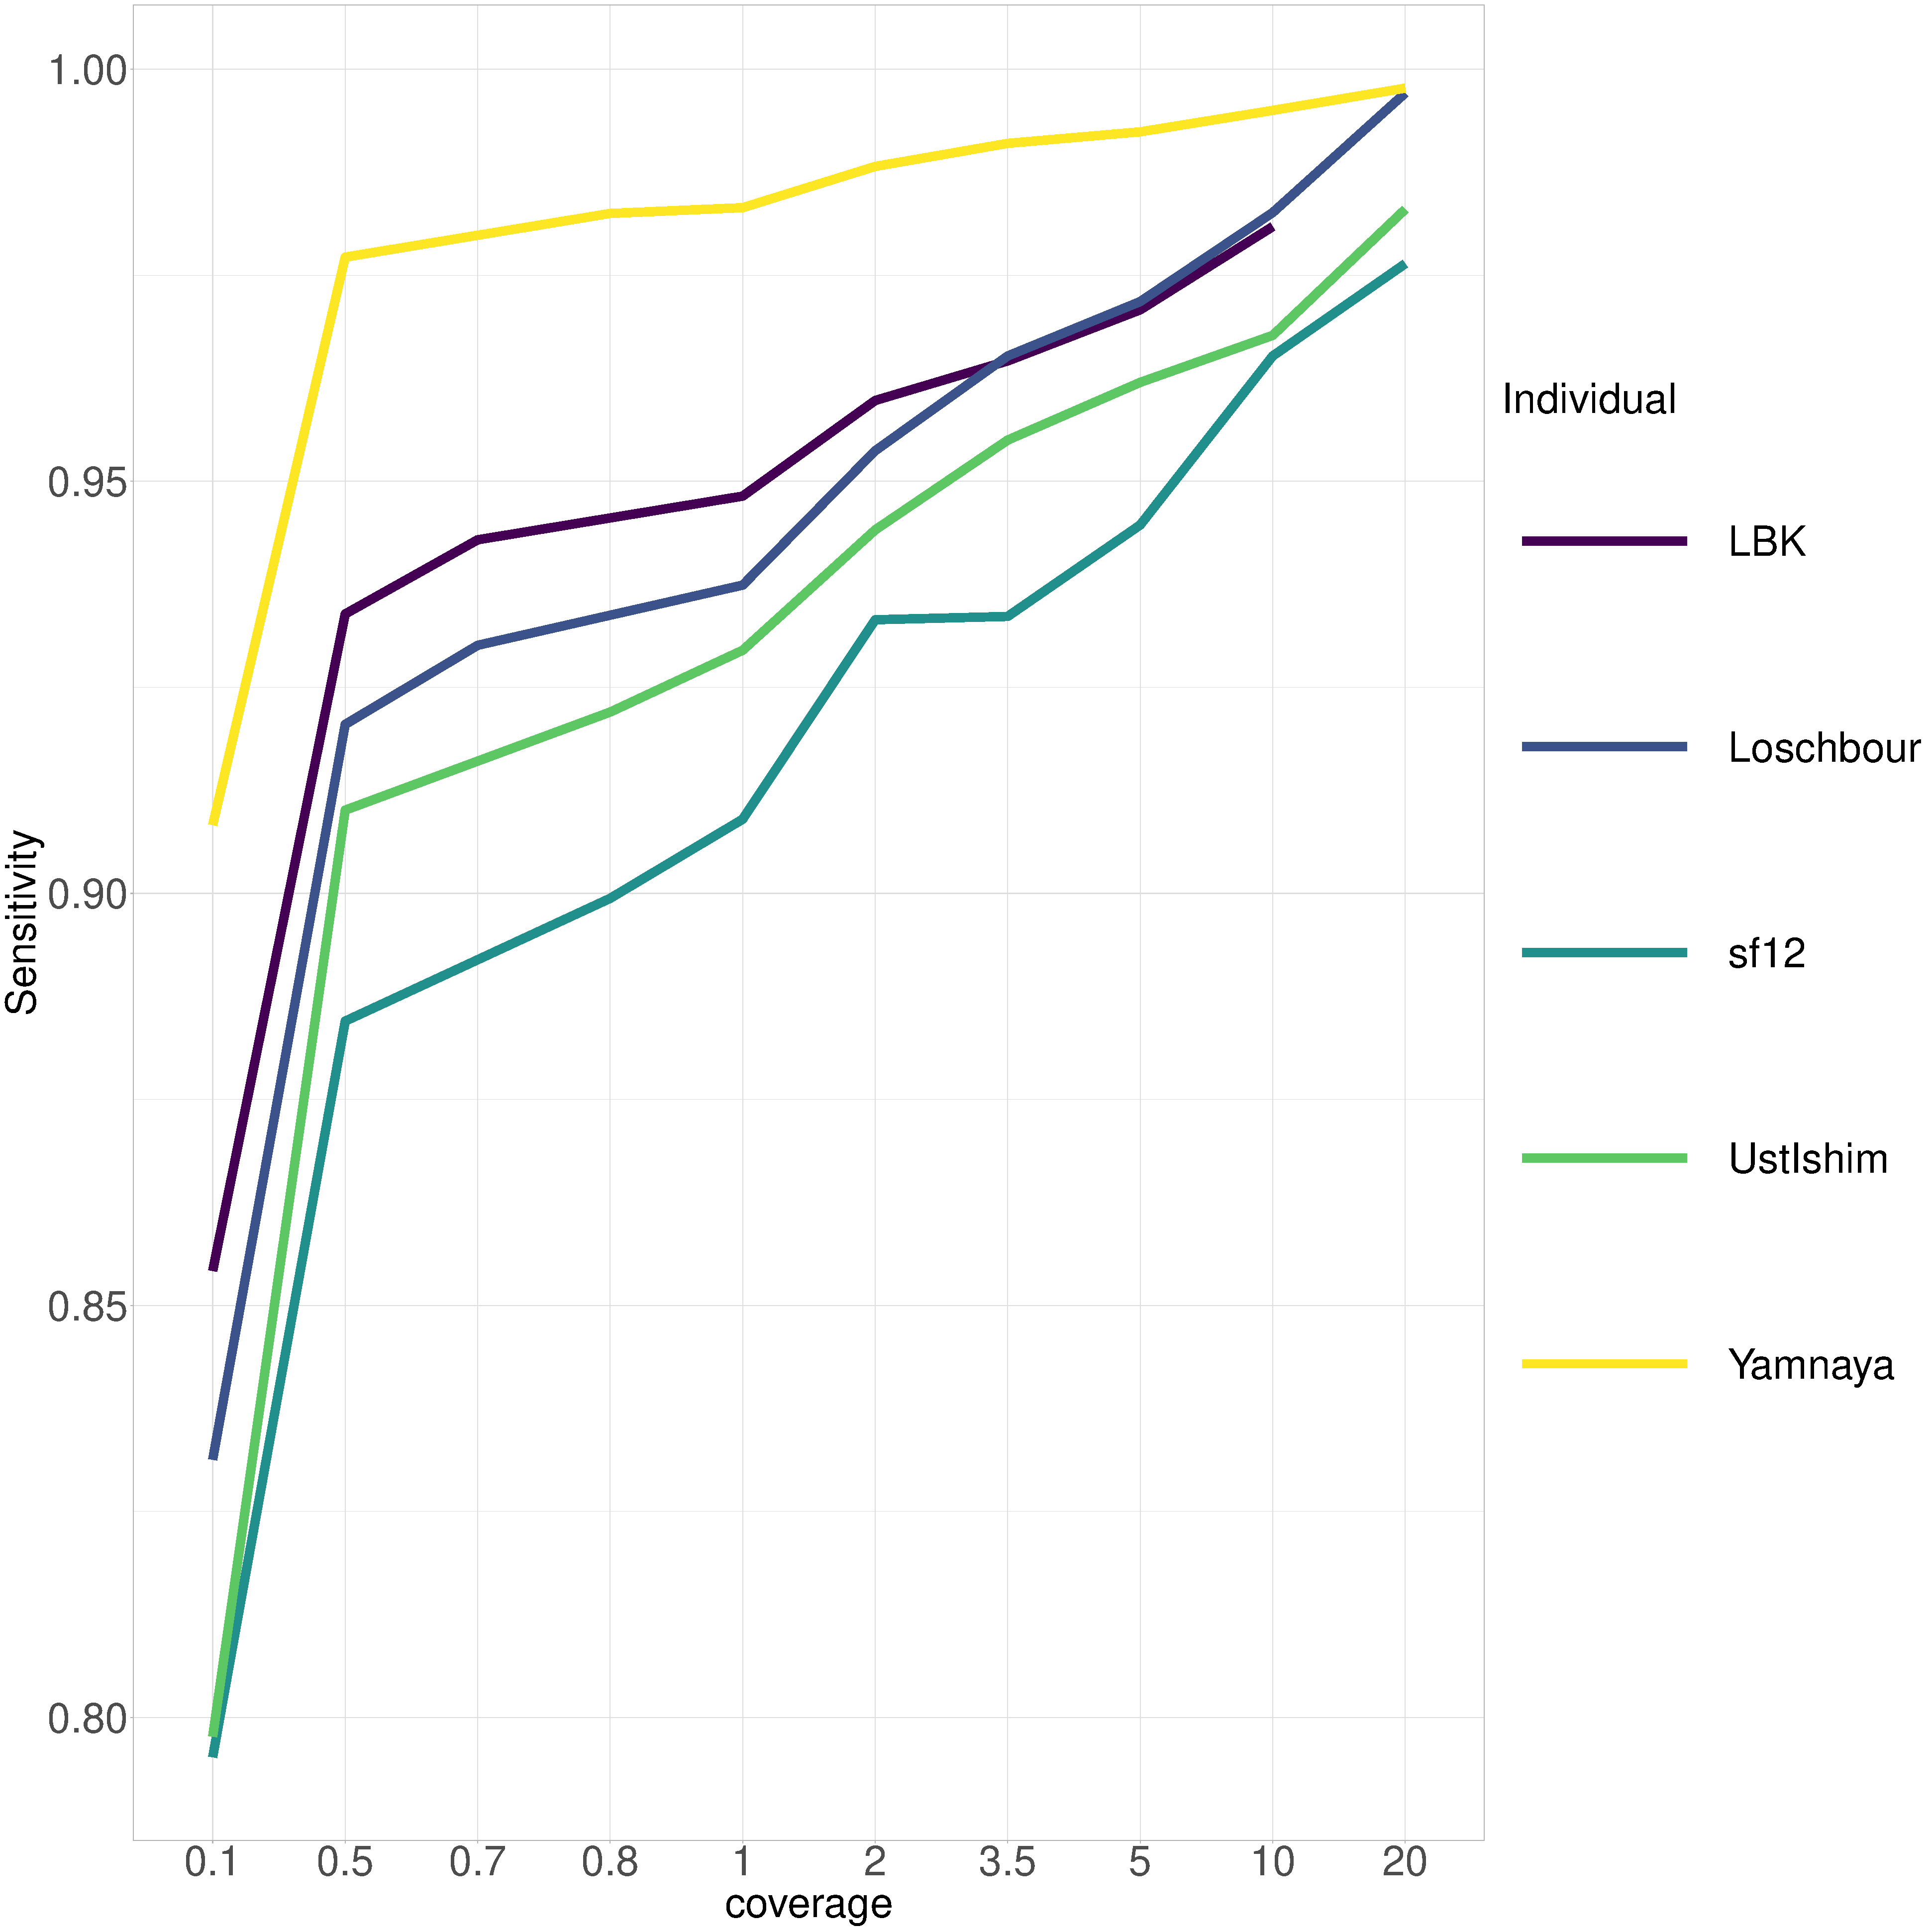
\includegraphics[width=1.0\textwidth]{../images/chapter1/allDownsampled_rtgtools_sensitivity.pdf}
    \caption{Sensitivity of genotype calling at different coverages for different ancient individuals.  calculated using rtg-tools. Calculated relative to the full coverage genome.}
    \label{fig:Sensitivity_downsampled_rtgtools}
\end{figure}

\begin{figure}[htp]
    \centering
    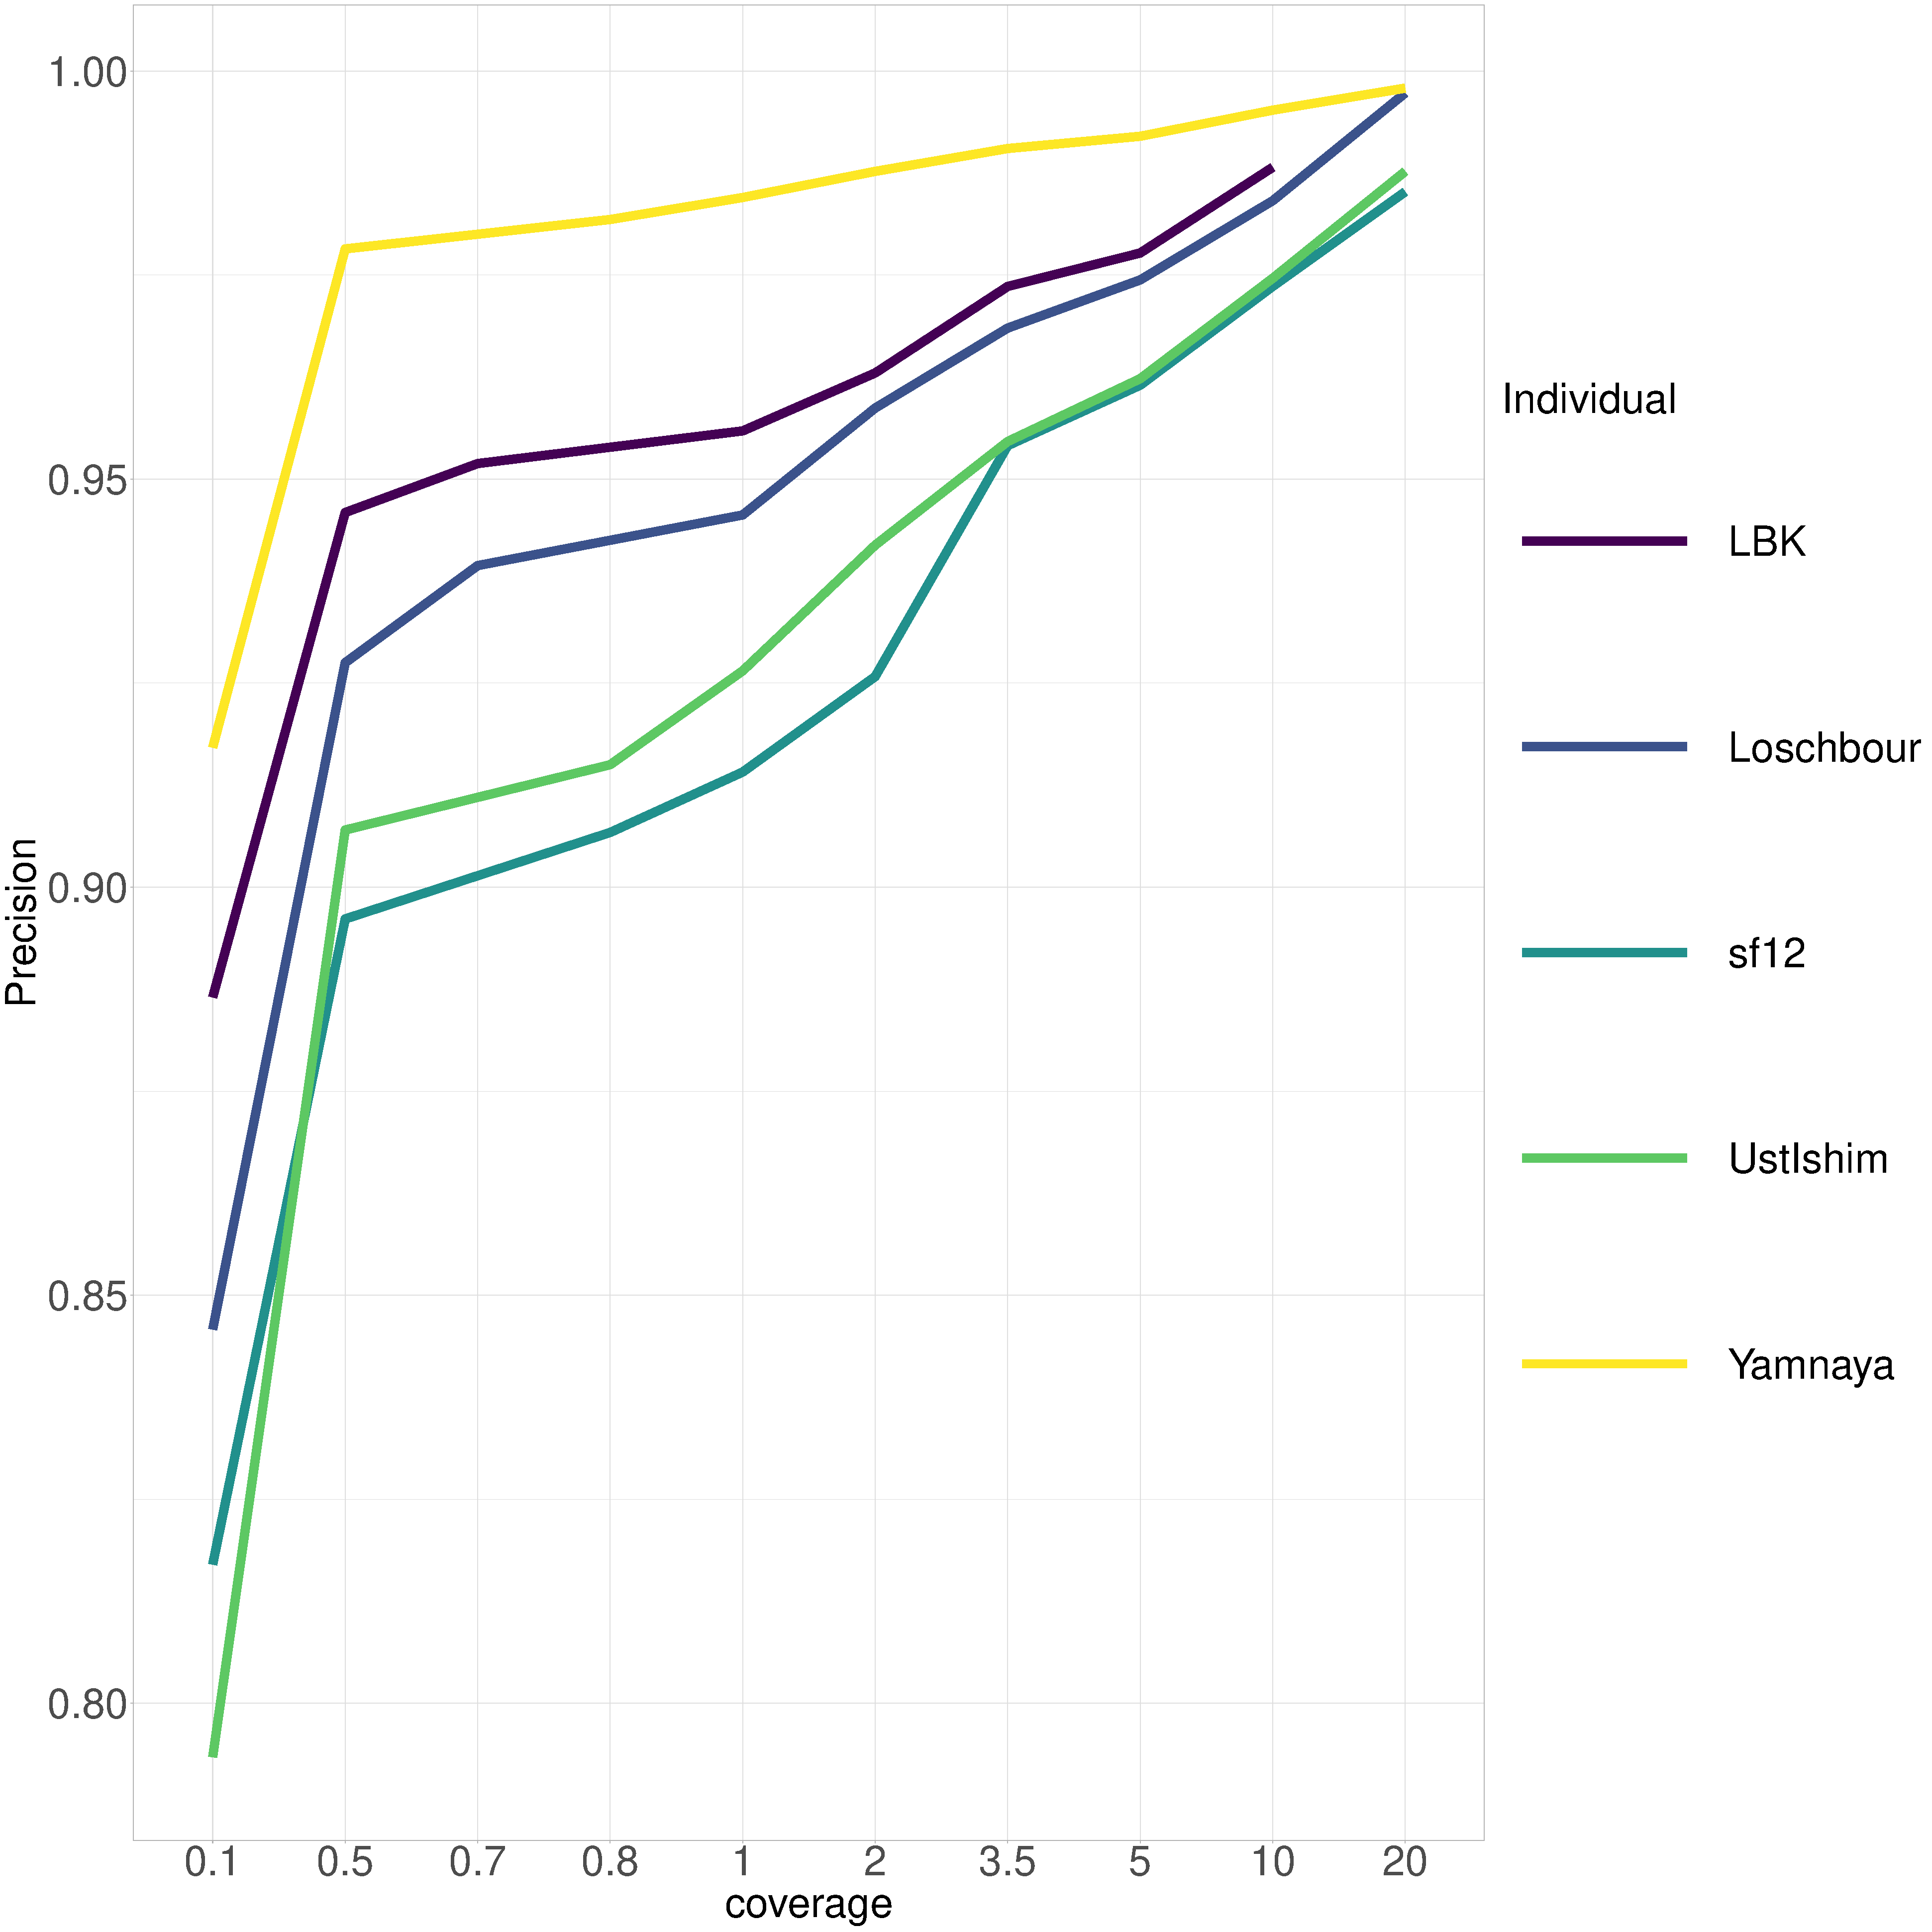
\includegraphics[width=1.0\textwidth]{../images/chapter1/allDownsampled_rtgtools_Precision.pdf}
    \caption{Precision of genotype calling at different coverages for different ancient individuals.  calculated using rtg-tools. Calculated relative to the full coverage genome.}
    \label{fig:precision_downsampled_rtgtools}
\end{figure}

As expected, both the overall sensitivity and precision of imputation fell with coverage, with a particularly sharp drop-off in both metrics observed at between 0.5x and 0.1x coverage.

The different downsampled individuals also differed in the precision and sensitivity for the genotype imputation. At all coverages, Yamnaya had the both the highest sensitivity and precision. This could be caused by the imputation reference panel containing individuals who are genetically closer to Yamnaya than any other ancient individual. This is consistent with modern Europeans containing a high proportion of Yamnaya-like ancestry \cite{Haak2005}. Many studies in modern individuals have shown that imputation accuracy increases when more haplotypes which are close to the target individual are found in the reference pane \cite{HUANG2009235, delaneau2018integrative}. On the other hand, the sample Ust'Ishim is known to have contributed very little genetic ancestry to modern day populations \cite{Prufer2014} and will therefore likely have fewer closely matching haplotypes in the reference panel, and correspondingly lower imputation accuracy. 

Imputation accuracy may also be related to demographic history. Populations which are known to have smaller effective population size, such as Western-Hunter Gathers, also contain longer IBD tracts and fewer heterozygous positions. As imputation relies on matching long IBD tracts between individuals, imputation accuracy increases where individuals share more IBD \cite{kong2008detection}. Additionally, switch-errors during the pre-phasing step of imputation may harm imputation accuracy, so a reduced density of heterozygous positions can improve accuracy. Put together, both of these facts suggest that it is possible to impute variants accurately in e.g. WHG, despite being less well represented in the reference panel.  

\subsection{Phasing accuracy}

I used rtg-tools to calculate the number of phased heterozygous genotypes where the downsampled individual has the same phasing as the full coverage individual. (Fig.  \ref{fig:phasing_performance_downsampled}). I note that this should not be considered to be the same as estimating the switch error rate, since we do not know that the phasing in the full-coverage individual is the true phase. However, this can be used as a rough proxy for switch errors, since it is known that phasing in lower coverage individuals is likely to be less accurate than those in the high coverage individuals \cite{rubinacci2021efficient}.

\begin{figure}[htp]
    \centering
    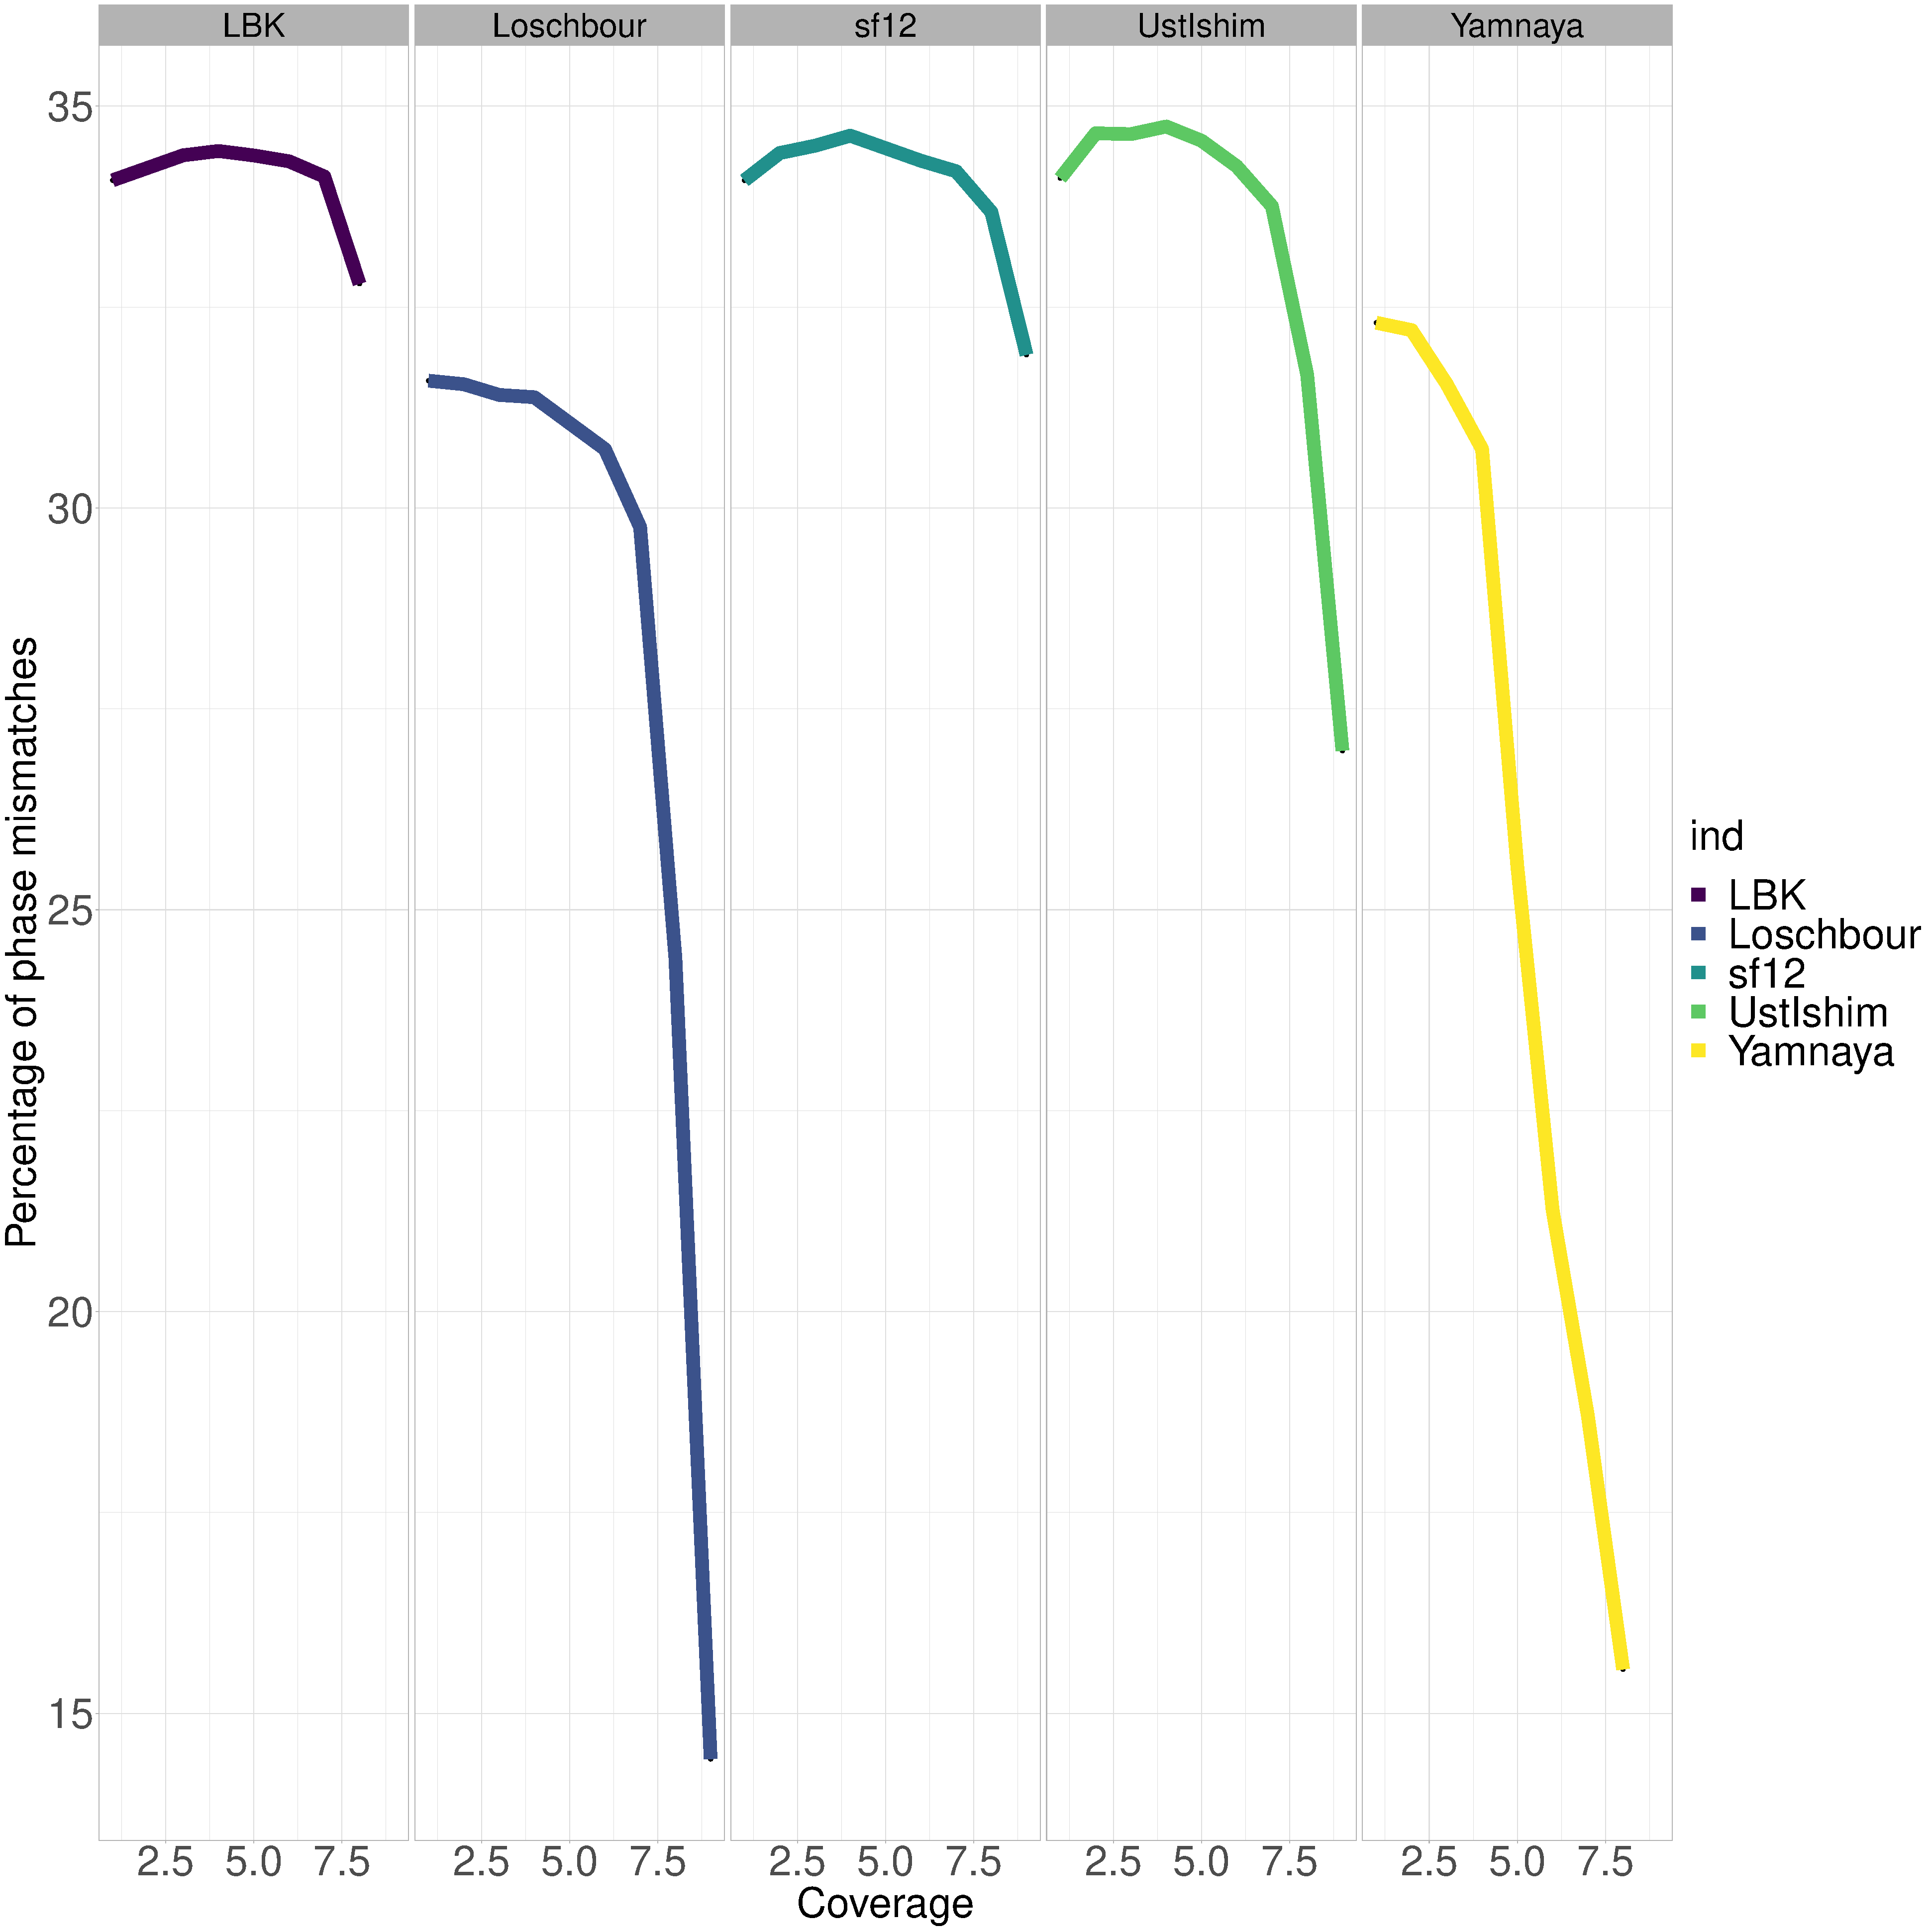
\includegraphics[width=1.0\textwidth]{../images/chapter1/phasing_performance_downsampled.pdf}
    \caption{Percentage of phased genotypes which agree with the reference for each individual and each level of downsampling. Genotypes with phase deemed 'unresolvable' by rtg-tools were excluded from the calculations. Note that these numbers are given as incorrect / incorrect + correct - unresolved and so values are in part driven by the relative heterozygosity of each sample.}
    \label{fig:phasing_performance_downsampled}
\end{figure}

\subsection{Validating posterior probability calibration}

The posterior genotype probabilities emitted by GLIMPSE give the posterior probability that a given genotype is the correctly called. Genotype probabilities are important for downstream analysis, particularly for deciding which variants to filter. However, it is important to validate that they are well calibrated (i.e. that they accurately reflect the probability a genotype call is correct).

To validate the genotype likelihoods, I took a single downsampled individuals (Yamnaya to 0.1x) and took the maximum genotype likelihood at each of the approximately 77 million positions which were processed by GLIMPSE. A $max(GL)$ for a particular genotype (i.e. 0.99) corresponds to a high confidence in the genotype. Alternatively a flat genotype likelihood (i.e. 0.33) corresponds to no information about the genotype. I performed the same analysis using different samples at different levels of coverage and the results were qualitatively similar. 

I then split the genome into 10,000 bins according to $max(GL)$. For each bin, I calculated both the proportion of SNPs which were correctly imputed (i.e. that matched the same high coverage individual) and the mean $max(GL)$ (Fig. \ref{fig:Yamnaya_0.1x_GL_calibration}). If the genotype probabilities are well calibrated, we would expect to see a clear positive linear relationship between $max(GL)$ probability and the probability that genotype matches the full-coverage sample.  

\begin{figure}[htp]
    \centering
    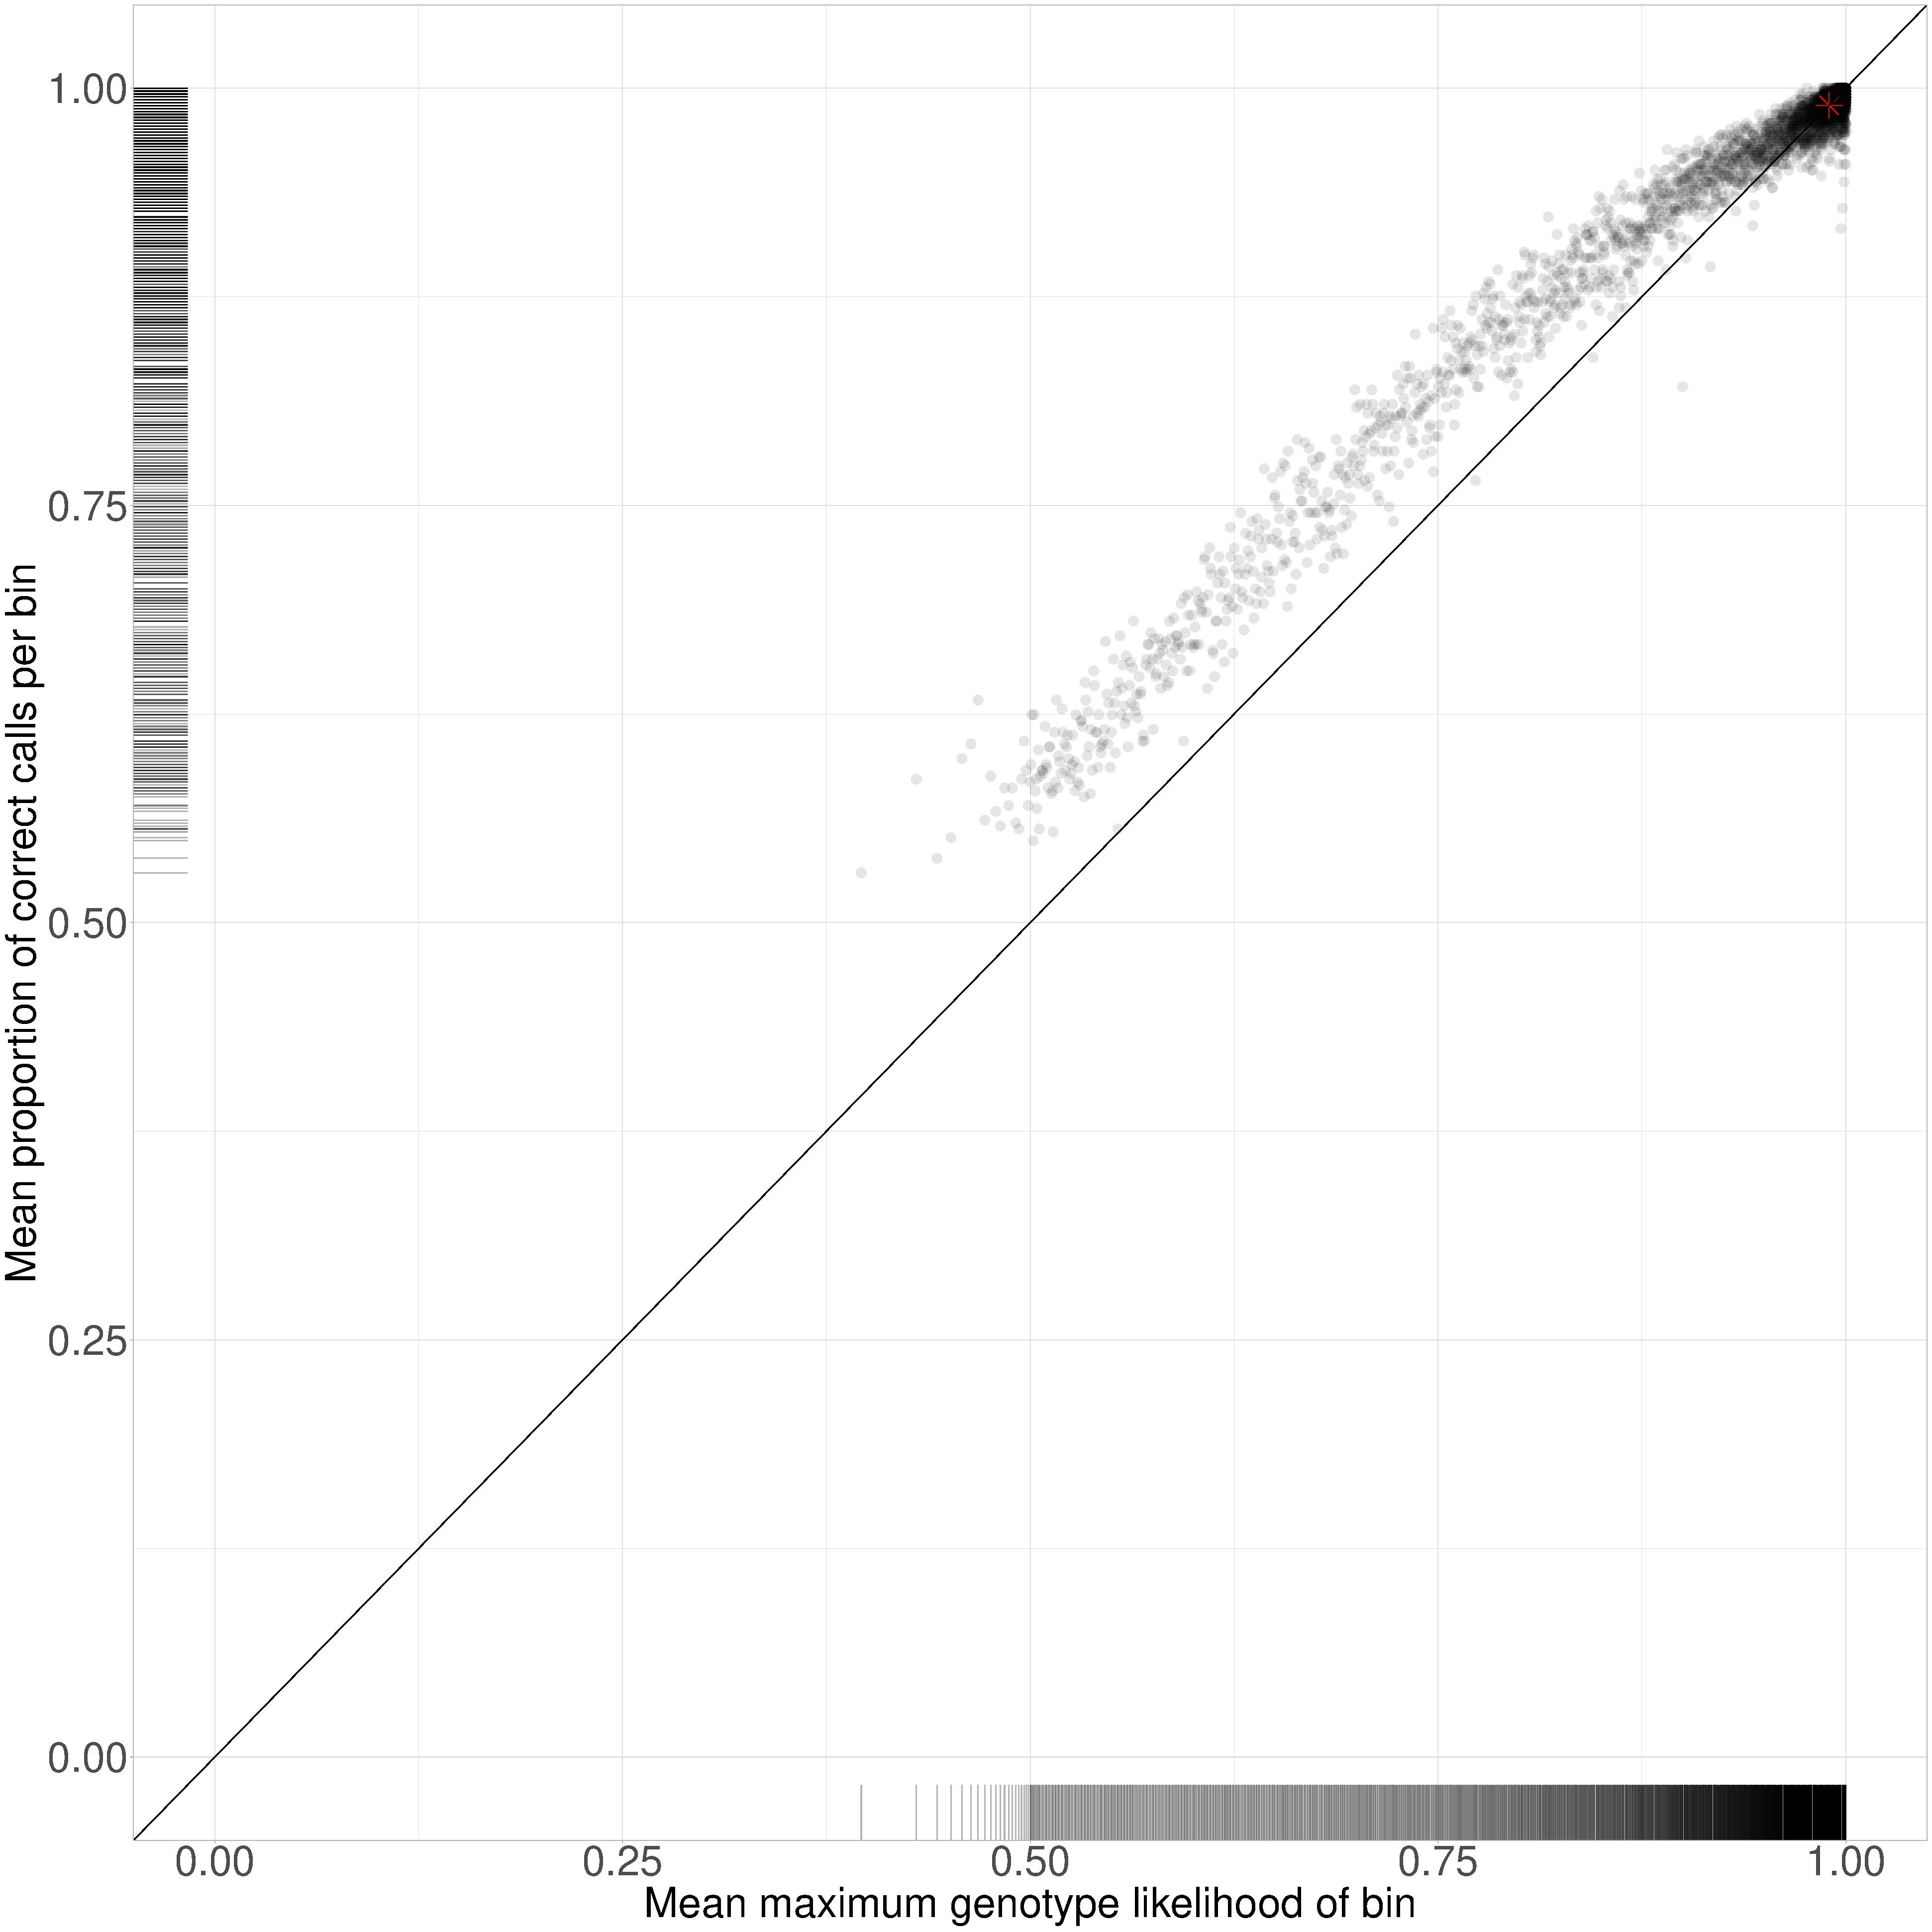
\includegraphics[width=1.0\textwidth]{../images/chapter1/Yamnaya_0.1x_bin.pdf}
    \caption{Relationship between genotype likelihood and probability of genotype call being correct. Genome binned by maximum posterior genotype likelihood and mean maximum posterior genotype likelihood (x-axis) and proportion of correct calls per bin (y-axis). Rugs on each margin show the distribution of x and y values. Black line is $y=x$.}
    \label{fig:Yamnaya_0.1x_GL_calibration}
\end{figure}

The figure confirms that the posterior genotype probabilities are well calibrated. They are slightly conservative, in that a majority of the points in Fig. \ref{fig:Yamnaya_0.1x_GL_calibration} are above the $y=x$ line. For example, the mean proportion of correct genotypes within all bins where $0.73 < max(GL) < 0.76$ was 82\%.

\subsection{ChromoPainter analysis}

I merged the dataset of downsampled individuals with the 'standard set' of reference individuals. I performed an all-v-all painting of the merged individuals, which compares each individual against each other individual in the dataset. I did this for both the standard version and uncertainty version of ChromoPainter.

I was interested how similar the copyvectors were between the full coverage and downsampled individuals. Copyvectors are vectors where each element contains the total length of genome a particular recipient most closely matches a particular donor individual. 

Fig. \ref{fig:CP_correlation_allSamples_0.1x_0.5x_30x} displays the relationship between copyvectors for each downsampled individual the corresponding full coverage individual for both 0.1x and 0.5x coverage. These results were obtained using the 30x 1000 genomes reference panel. 

\begin{figure}[htp]
    \centering
    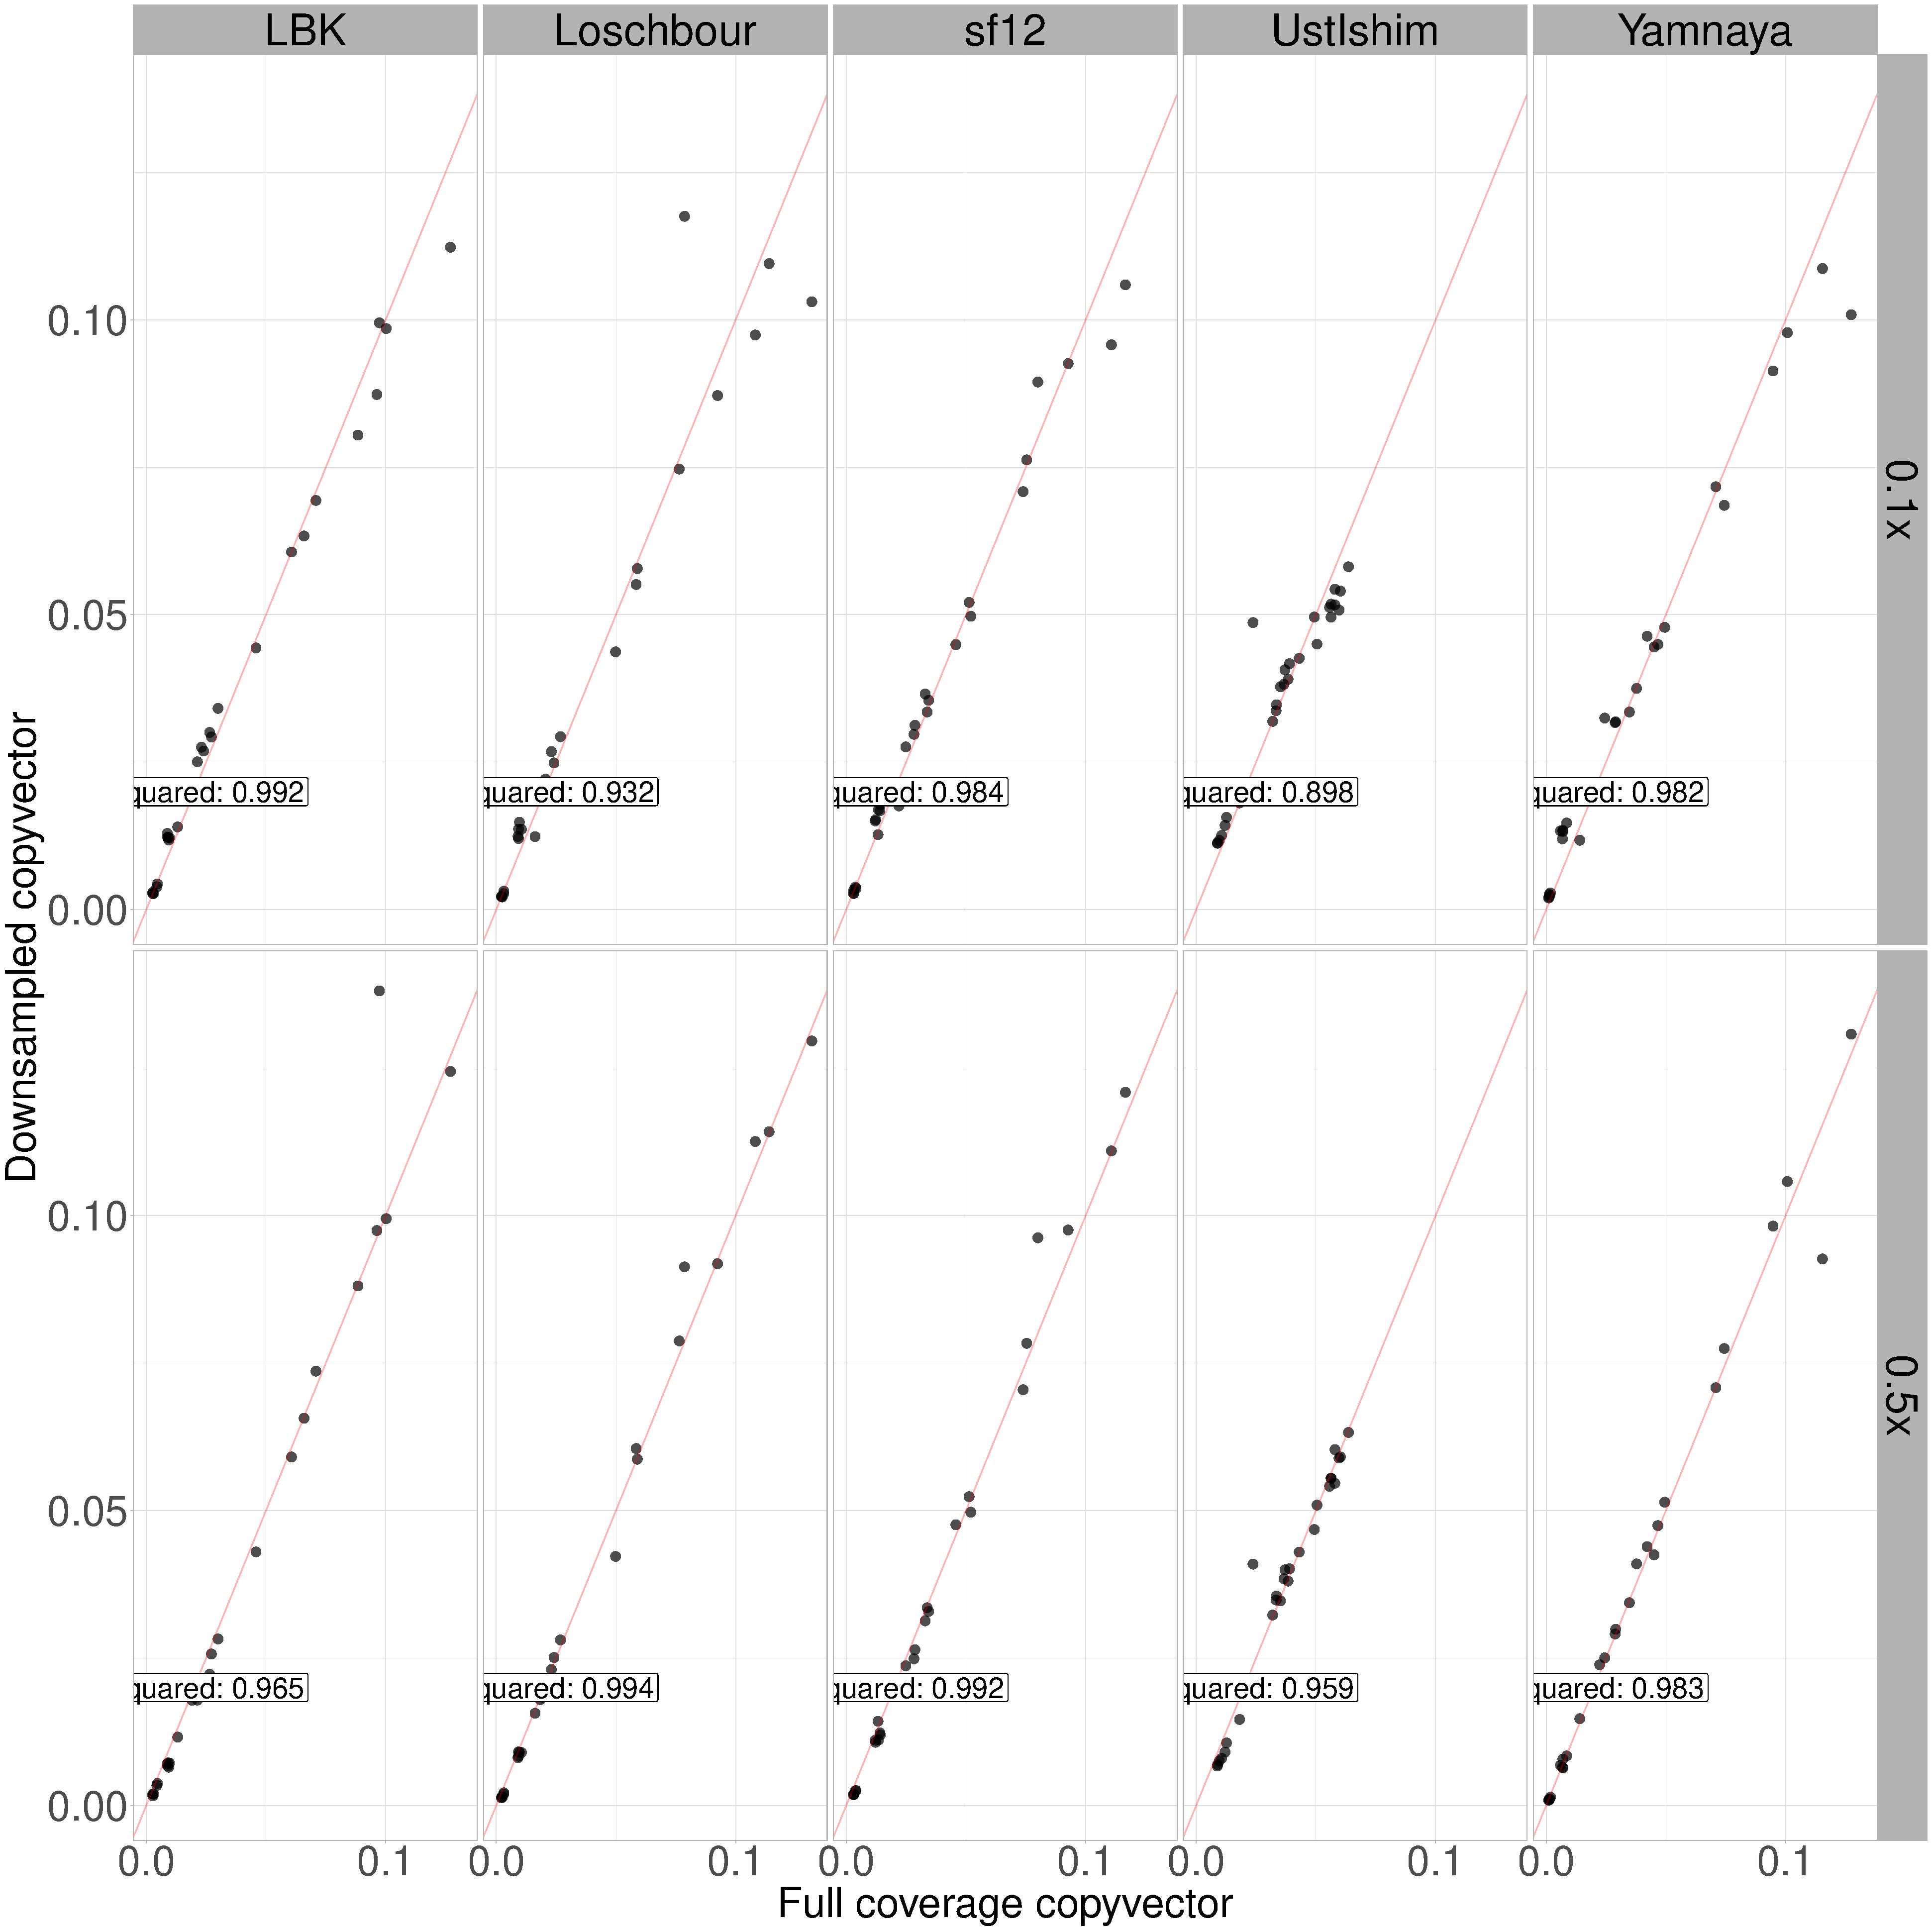
\includegraphics[width=1.0\textwidth]{../images/chapter1/CP_correlation_allSamples_0.1x_0.5x_30x.pdf}
    \caption{Relationship between normalised copyvectors between downsampled and full coverage individuals. Copyvectors estimated using 125 ancient donors.}
    \label{fig:CP_correlation_allSamples_0.1x_0.5x_30x}
\end{figure}

As expected, the r-squared value between the full-coverage and downsampled copyvectors increased with coverage. The 0.1x genome had a substantially reduced r-squared value, similar to the much reduced imputation accuracy. For each of the genomes downsampled to 0.1x, a particular difference to the 0.5x downsampled genomes is that, for each individual, the lowest contributing donors contribute more to the 0.1x downsampled genome than to the full coverage genome and that the highest contributing donors contribute less to the 0.1x genome than they do the full coverage genome. Put in other words, the copyvectors at 0.1x are tending towards coming more 'flat' or copying the same amount from each donor individual. This can be observed as the coefficients of the linear model lines on the figures are much less in the 0.1x than the 0.5x individuals. This can also be seen as 'regressing to the prior', where in this case, the prior is copying an equal amount to each donor individual. This can be visualised explicitly by calculating TVD between each downsampled genome and a flat prior, a vector of length $D$, where $D$ is the total number of donor individuals and each element of $D$ is equal to 1 / $D$ (Fig. \ref{fig:TVD_ancients_flat_prior}). This clearly shows the reduced TVD to the flat copyvector for the 0.1x individual relative to other coverages.

\begin{figure}[htp]
    \centering
    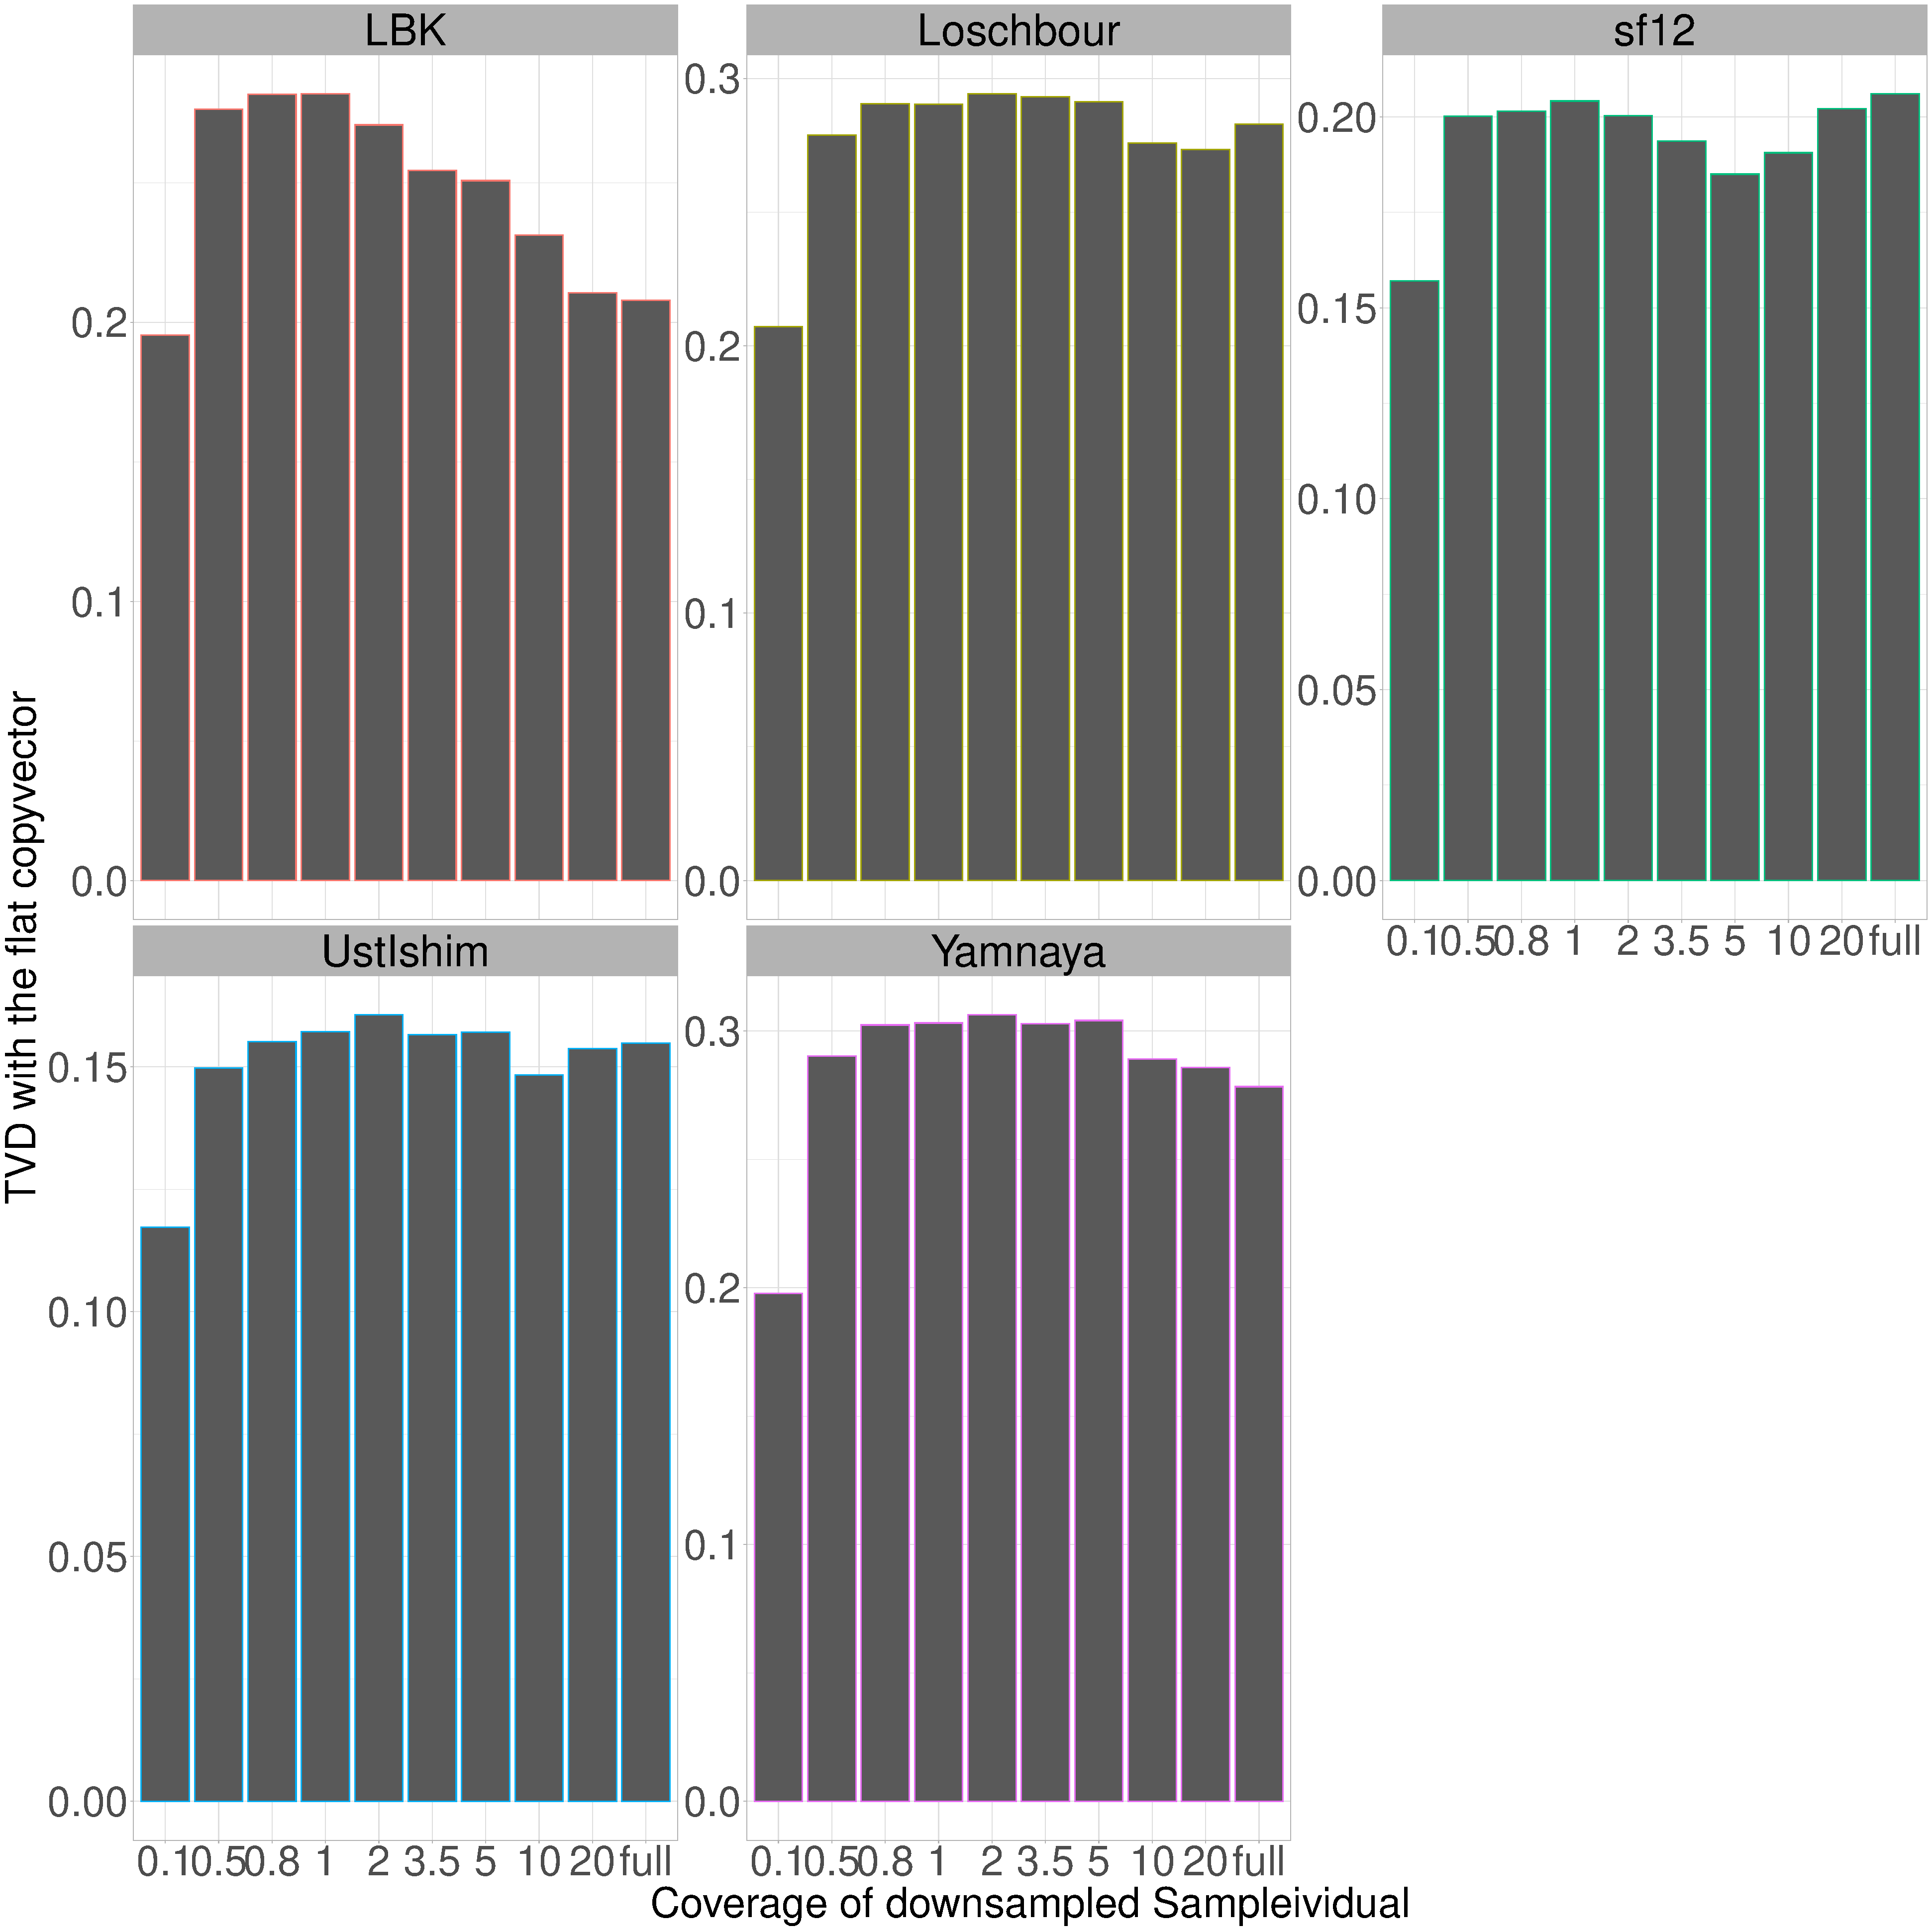
\includegraphics[width=1.0\textwidth]{../images/chapter1/TVD_ancients_flat_prior.pdf}
    \caption{TVD (metric of copyvector dissimilarity between two individuals) between each downsampled ancient individual and a flat copyvector. Flat copyvector equivalent to a vector of length $N$ where each element = $1/N$.}
    \label{fig:TVD_ancients_flat_prior}
\end{figure}

I also considered the effect of coverage on the copyvectors estimated when using modern individuals as donors (Fig. \ref{fig:CP_correlation_allSamples_0.1x_0.5x_30x_moderns}). I merged the downsampled and full coverage ancient individuals with the 30x thousand genomes dataset (described in detail in appendix A.5). As was the case with the all-v-all ancients painting, the r-squared between copyvectors was lowest for the 0.1x individuals. However, the copyvectors show a strong correlation (all greater than 0.990) for 0.5x individuals.  

It should be noted that utility of painting different ancient individuals with a modern reference panel depends on the ancestry and age of the ancient sample. The spread of points along the $y=x$ line in Fig. \ref{fig:CP_correlation_allSamples_0.1x_0.5x_30x_moderns} shows how much a particular ancient recipient preferentially copies more from particular modern population over others. LBK, for example, has points which are spread evenly across $y=x$, showing that they copy much more from some populations than others, suggesting modern populations are good for distinguishing this particular ancient sample. On the other hand, the points for Ust'Ishim are clumped together along $y=x$, showing that the copyvector is relatively flat and that it does not preferentially copy from some populations to the same degree that LBK does. Accordingly, relatively less useful information is obtained from painting Ust'Ishim with a modern reference panel than LBK.

\begin{figure}[htp]
    \centering
    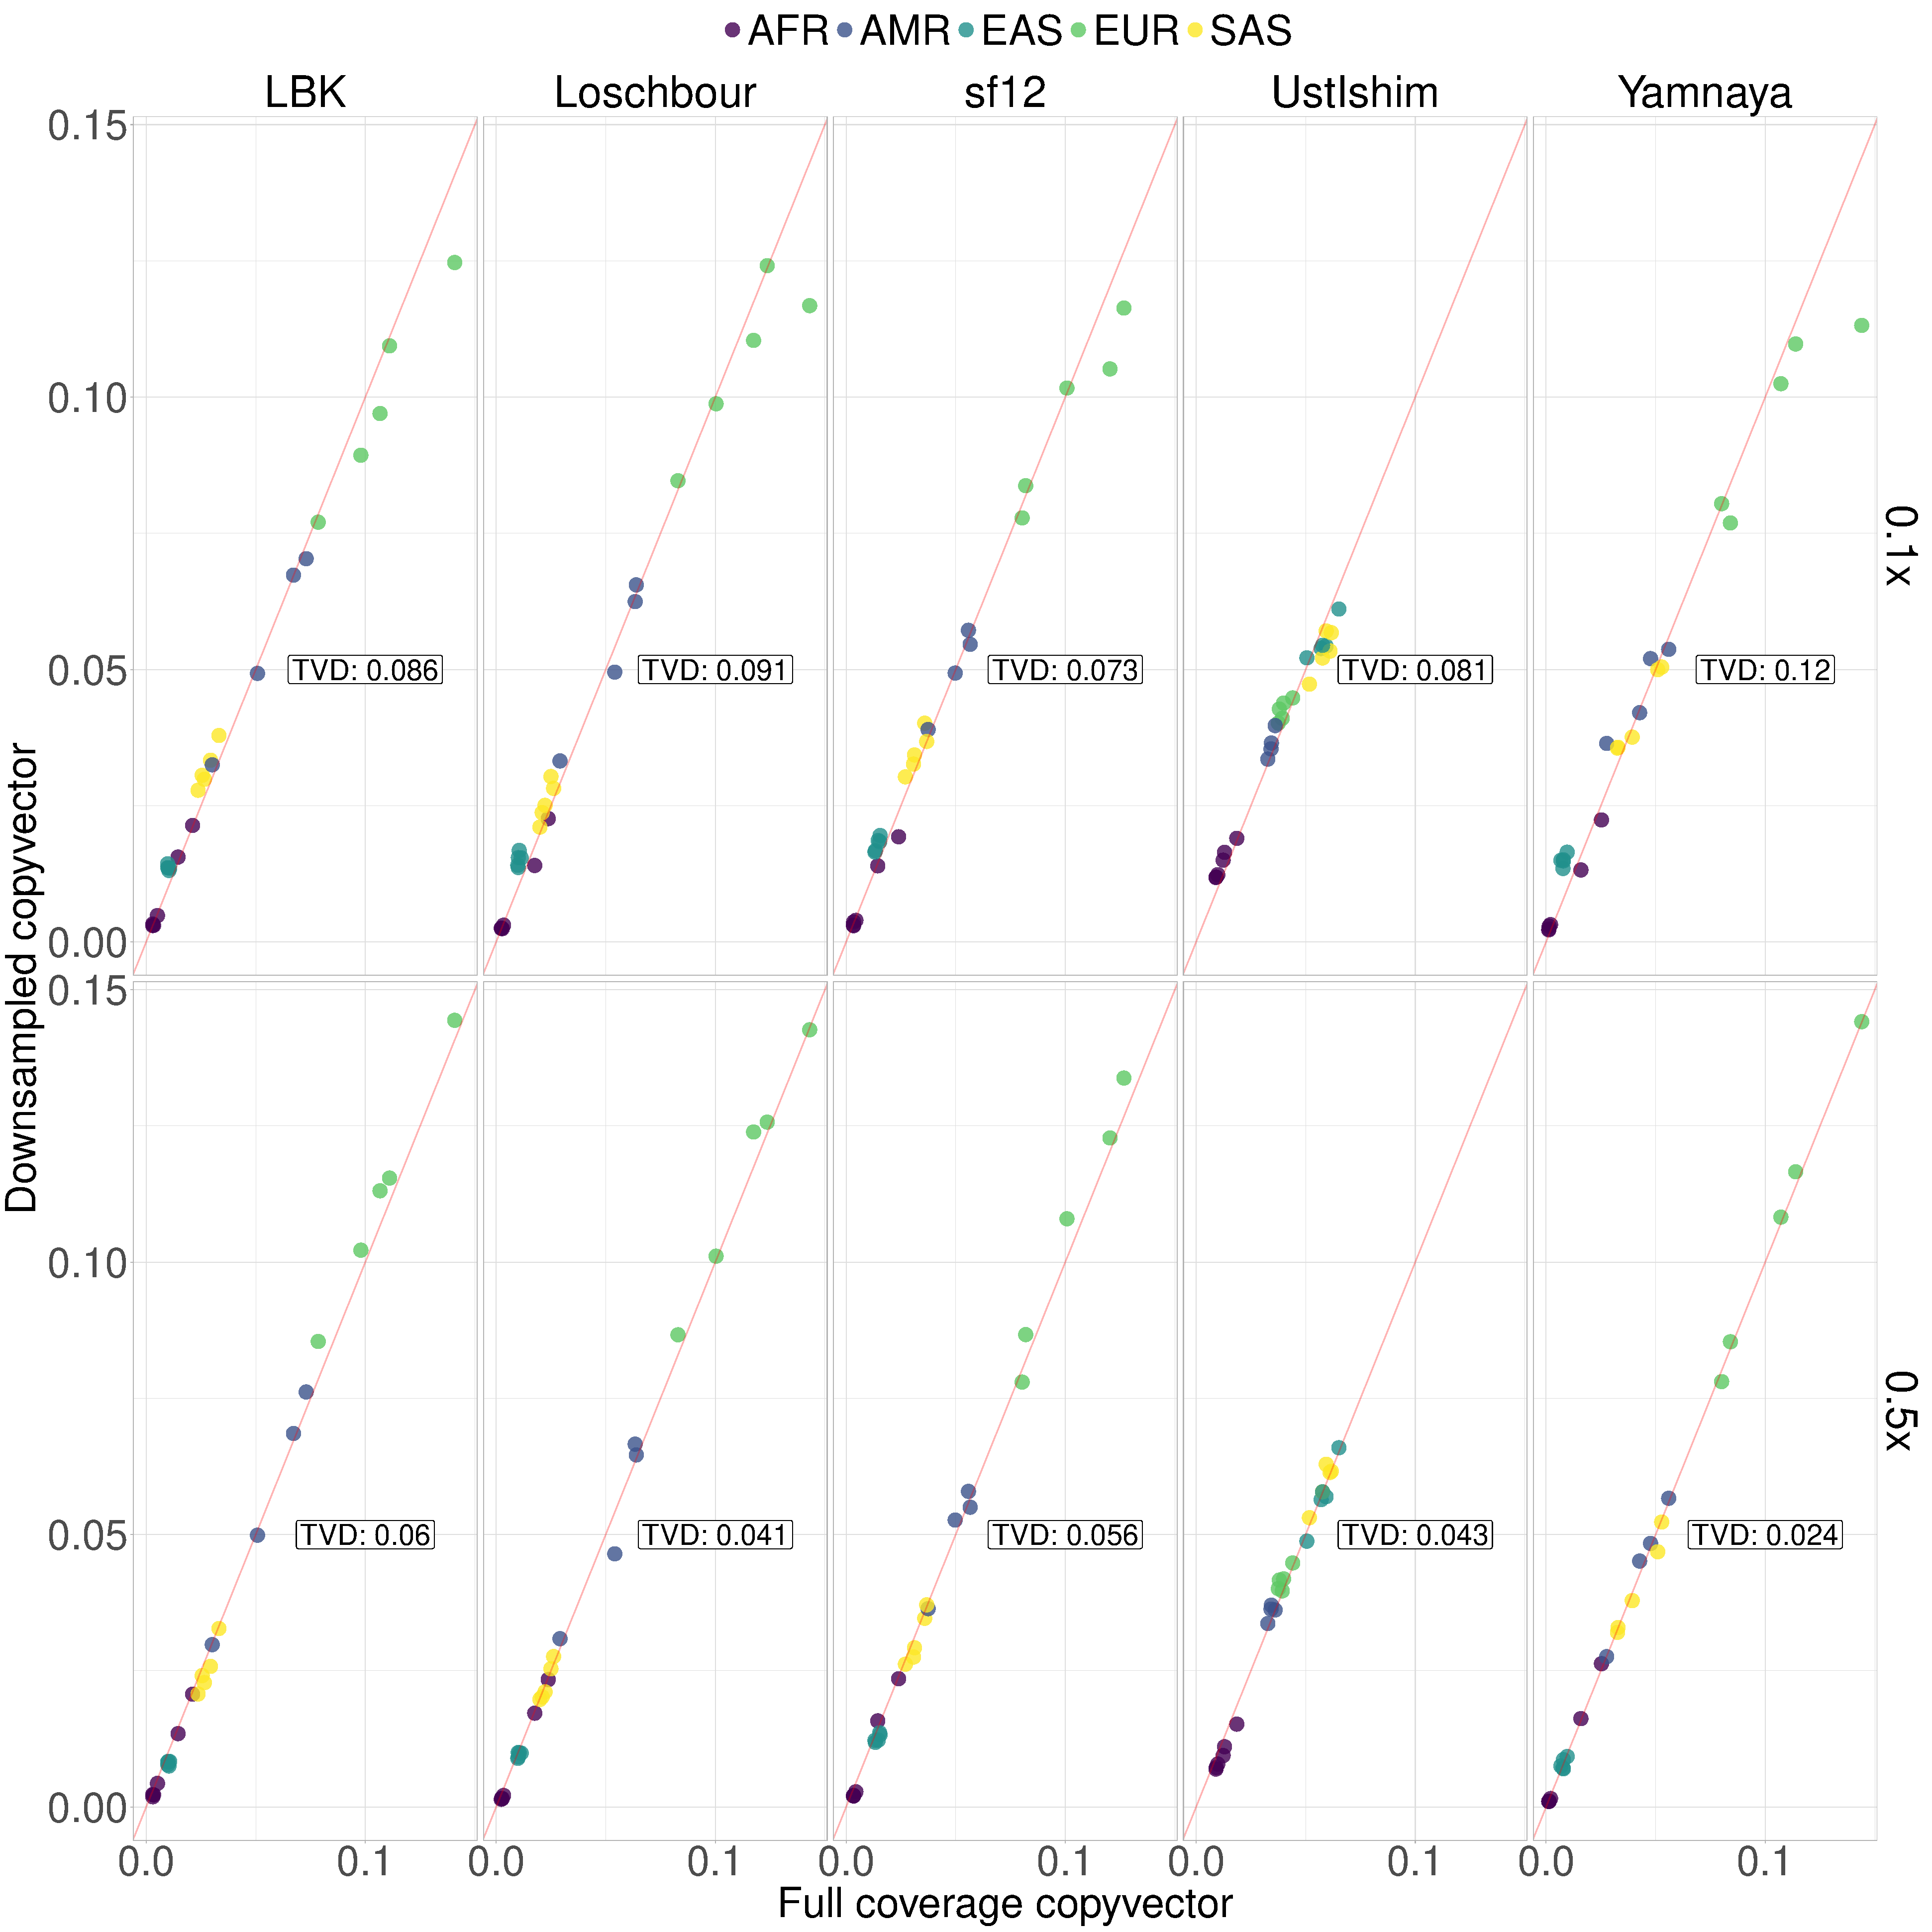
\includegraphics[width=1.0\textwidth]{../images/chapter1/CP_correlation_allSamples_0.1x_0.5x_30x_moderns.pdf}
    \caption{Relationship between normalised copyvectors between downsampled and full coverage individuals. Copyvectors estimated using 3203 modern donors grouped into 26 populations.}
    \label{fig:CP_correlation_allSamples_0.1x_0.5x_30x_moderns}
\end{figure}

Principle component analysis (PCA) is a widely used technique to visualise the relative ancestry of individuals. PCA can be performed on the chunklengths matrix in a similar way to a PCA on the genotype dosage matrix. I performed PCA on each chunklengths matrix to visualise the positions of the full coverage and downsampled genomes. PCA was performed on the chunklengths matrix containing all individuals. To avoid the confounding effect of having two almost identical individuals on a PCA (i.e. the 1x and 0.5x downsample of the same individual) I performed PCA separately for each ancient individual and plotted the loadings for PC1 and PC2 for each ancient downsampled, full coverage and reference individual, on the same plot (Fig. \ref{fig:PCA_panel_allInds_allCoverage}).The positions of the full coverage and downsampled genome corresponds to the similarity in copyvectors relative to other samples in the PCA. When the full coverage and downsampled genome are positioned close to one another, it suggests that coverage has not affected the copyvector estimation. 

The position of the downsampled individuals is consistent with prior knowledge about their ancestry; Loschbour is positioned alongside other Hunter Gatherers who are highly differentiated from the later neolithic farmers and Bronze Age Europeans. sf12 clusters with the other Scandinavian Hunter Gatherers in the dataset. Yamnaya is differentiated from the group of Bronze Age individuals and situated close to individuals from the Poltavka and Srubnaya culture. LBK is located with other individuals from the early to middle Neolithic in central Europe. Consistent with sharing little ancestry with any group over another, UstIshim is positioned close to the central Bronze Age mass where most of the individuals in the PCA are located (I presume this is because UstIshim has a relatively flat copyvector and therefore is positioned near to where most of these samples are). 

For all levels of downsampling other than the 0.1x, the downsampled and full coverage genomes were positioned very closely to one another on the PCA. When considering all downsampled individuals, a pattern emerges whereby the genome downsampled to 0.1x for each individual is 'pulled' towards the origin of the PCA. This may reflect a 'homogenisation' of low coverage genomes when most of the positions are imputed. 

\begin{figure}[htp]
    \centering
    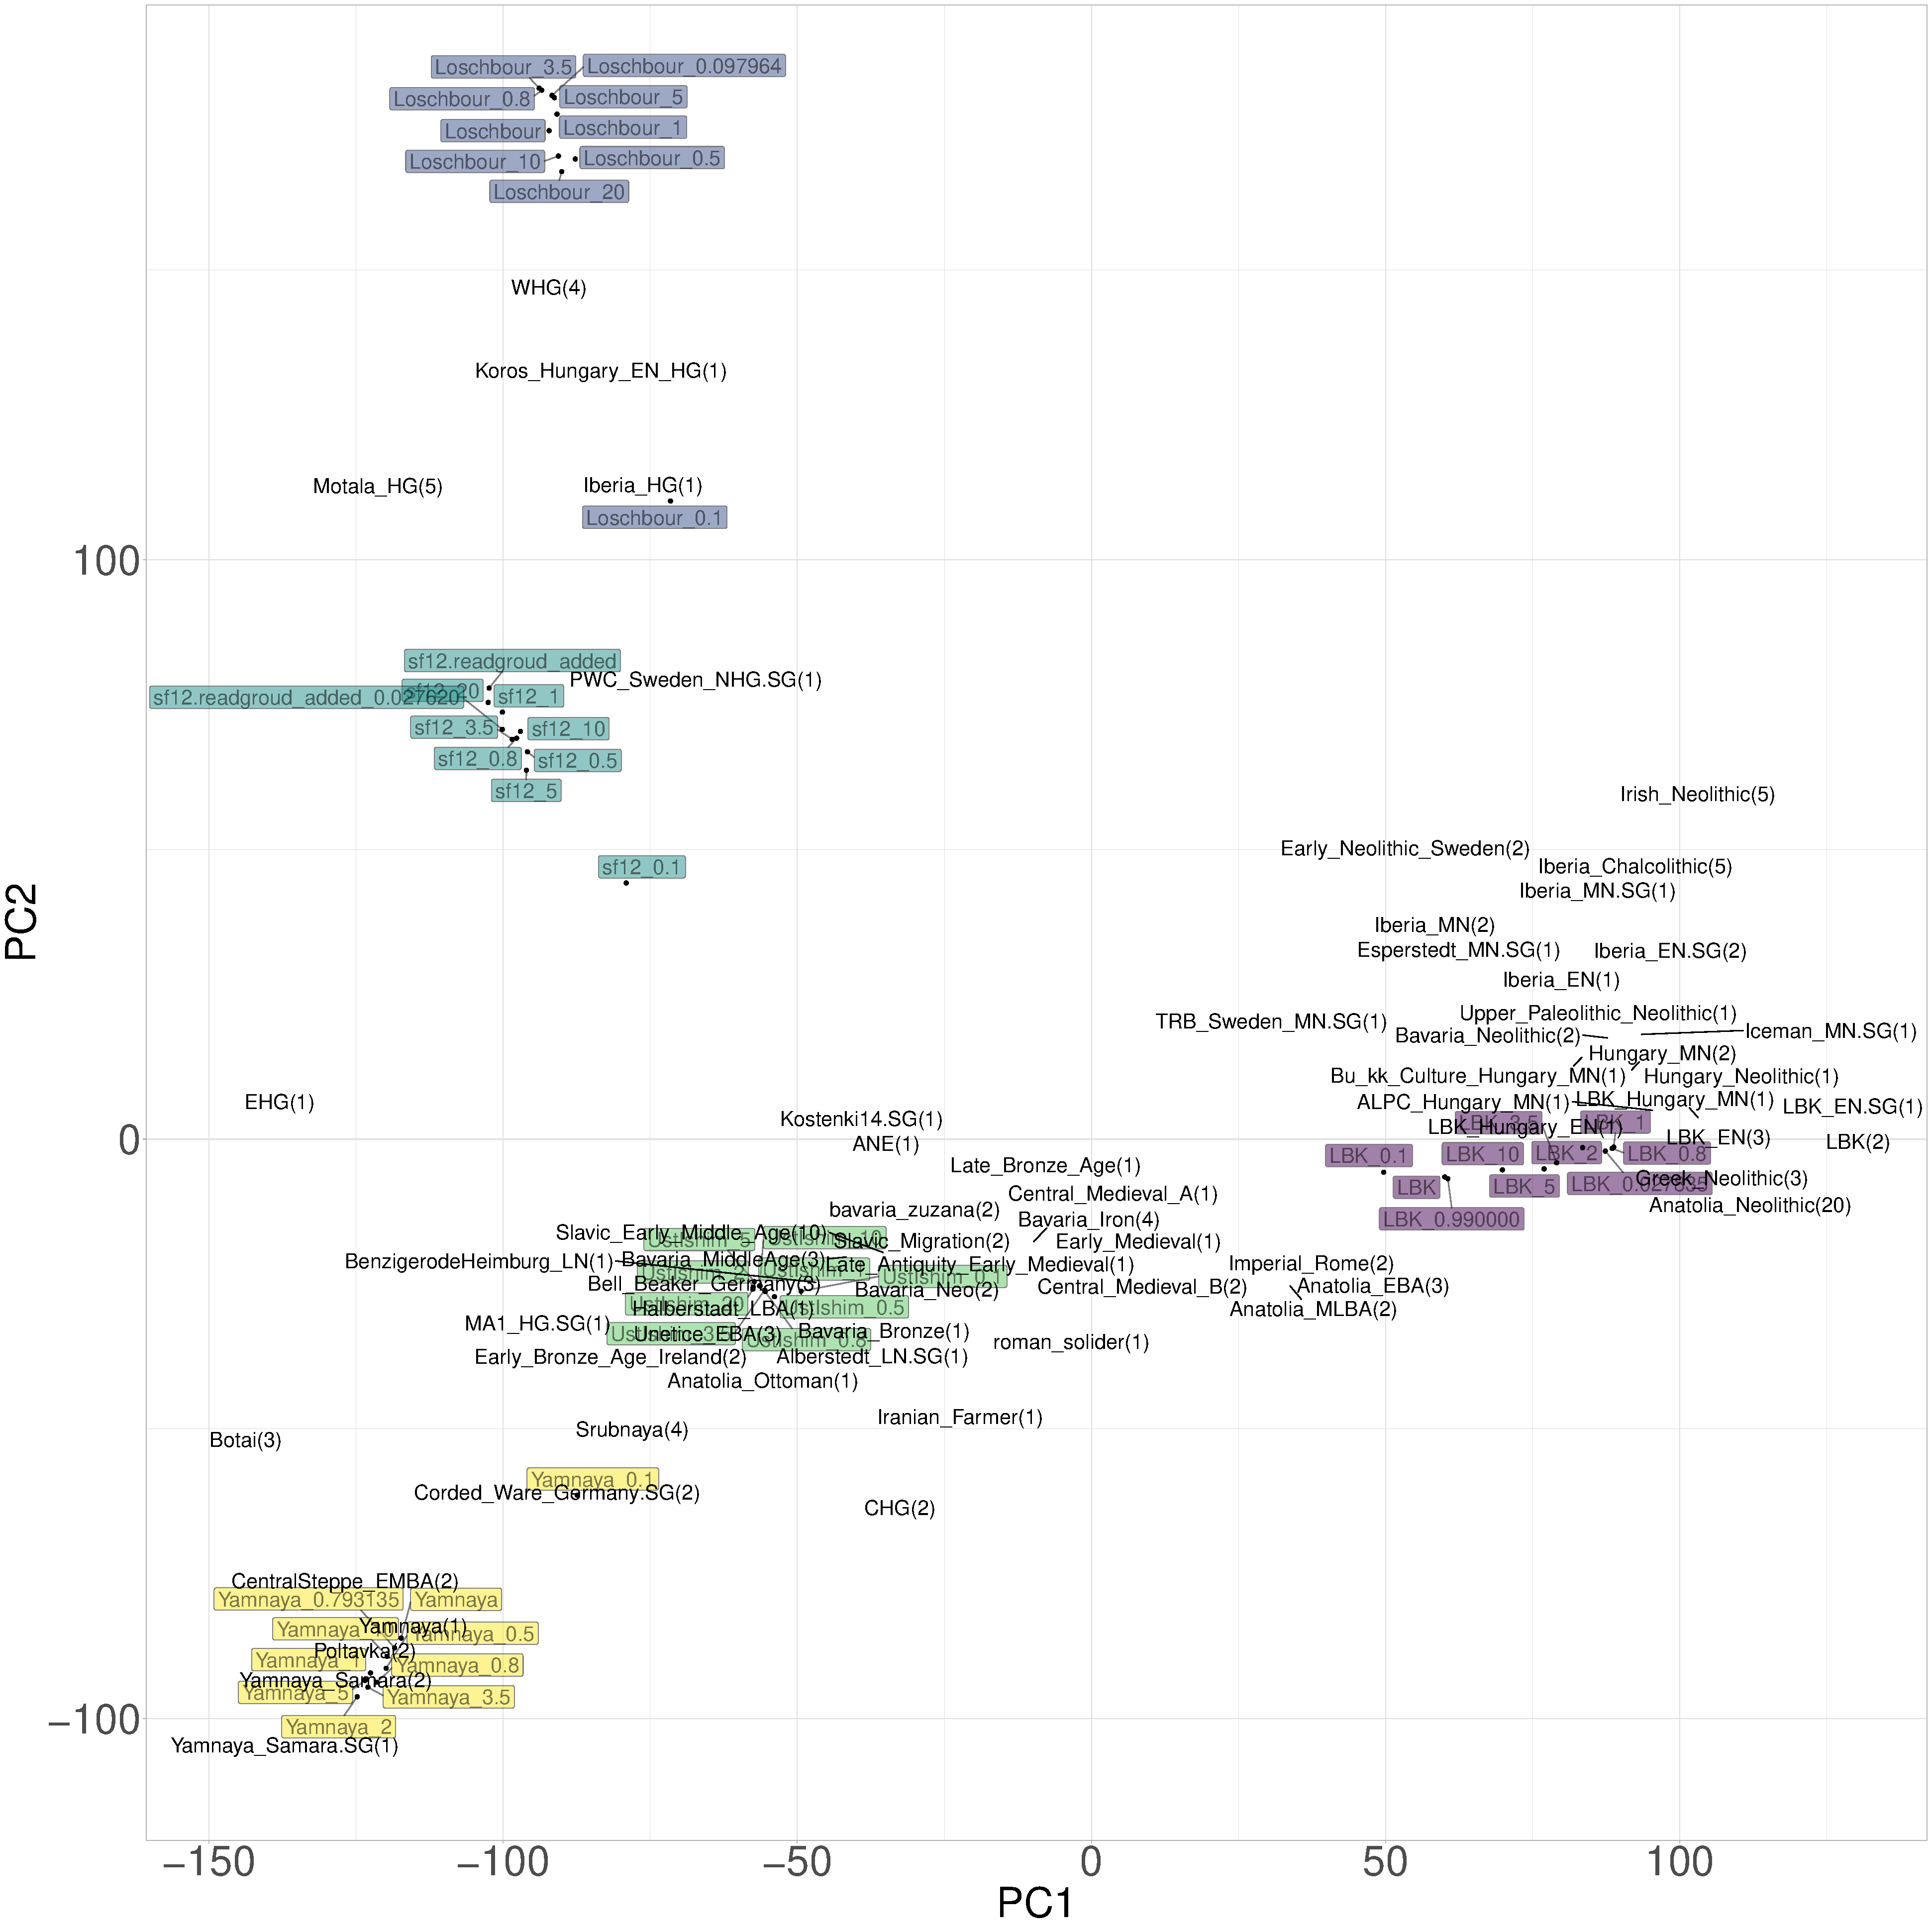
\includegraphics[width=1.0\textwidth]{../images/chapter1/PCA_panel_allInds.allCoverage.pdf}
    \caption{Principle component analysis (PCA) of downsampled, full coverage and reference ancient individuals generated from the linked chunklengths matrix. Full coverage and downsampled genomes of the same individual are coloured the same. Reference individuals are grouped into populations plotted as the mean principle components for all individuals within the population.}
    \label{fig:PCA_panel_allInds_allCoverage}
\end{figure}

Taken together, these data suggest minimal effect of coverage down to and including 0.5x.

\subsection{SOURCEFIND}

I next determined the effect of sequencing coverage on the ancestry proportions estimated by SOURCEFIND. The chunklengths matrix contains information about the total length of genome one particular individual most closely matches any other individual. However, this information is often noisy due to phenomena such as incomplete lineage sorting and variable donor group sizes. Therefore, it is often desirable to model out this noise and estimate ancestry proportions in each individual, which are cleaner and more interpretable than raw chunk lengths. 

I began by considering 3 ancestral sources, or 'surrogates', fixed as Anatolia Neolithic, Western Hunter-Gatherer and Yamnaya steppe pastoralist. I compared inferred proportions for the same individual across different levels of coverage (Fig. \ref{fig:3pop_SF_downsampled}). 

\begin{figure}[htp]
    \centering
    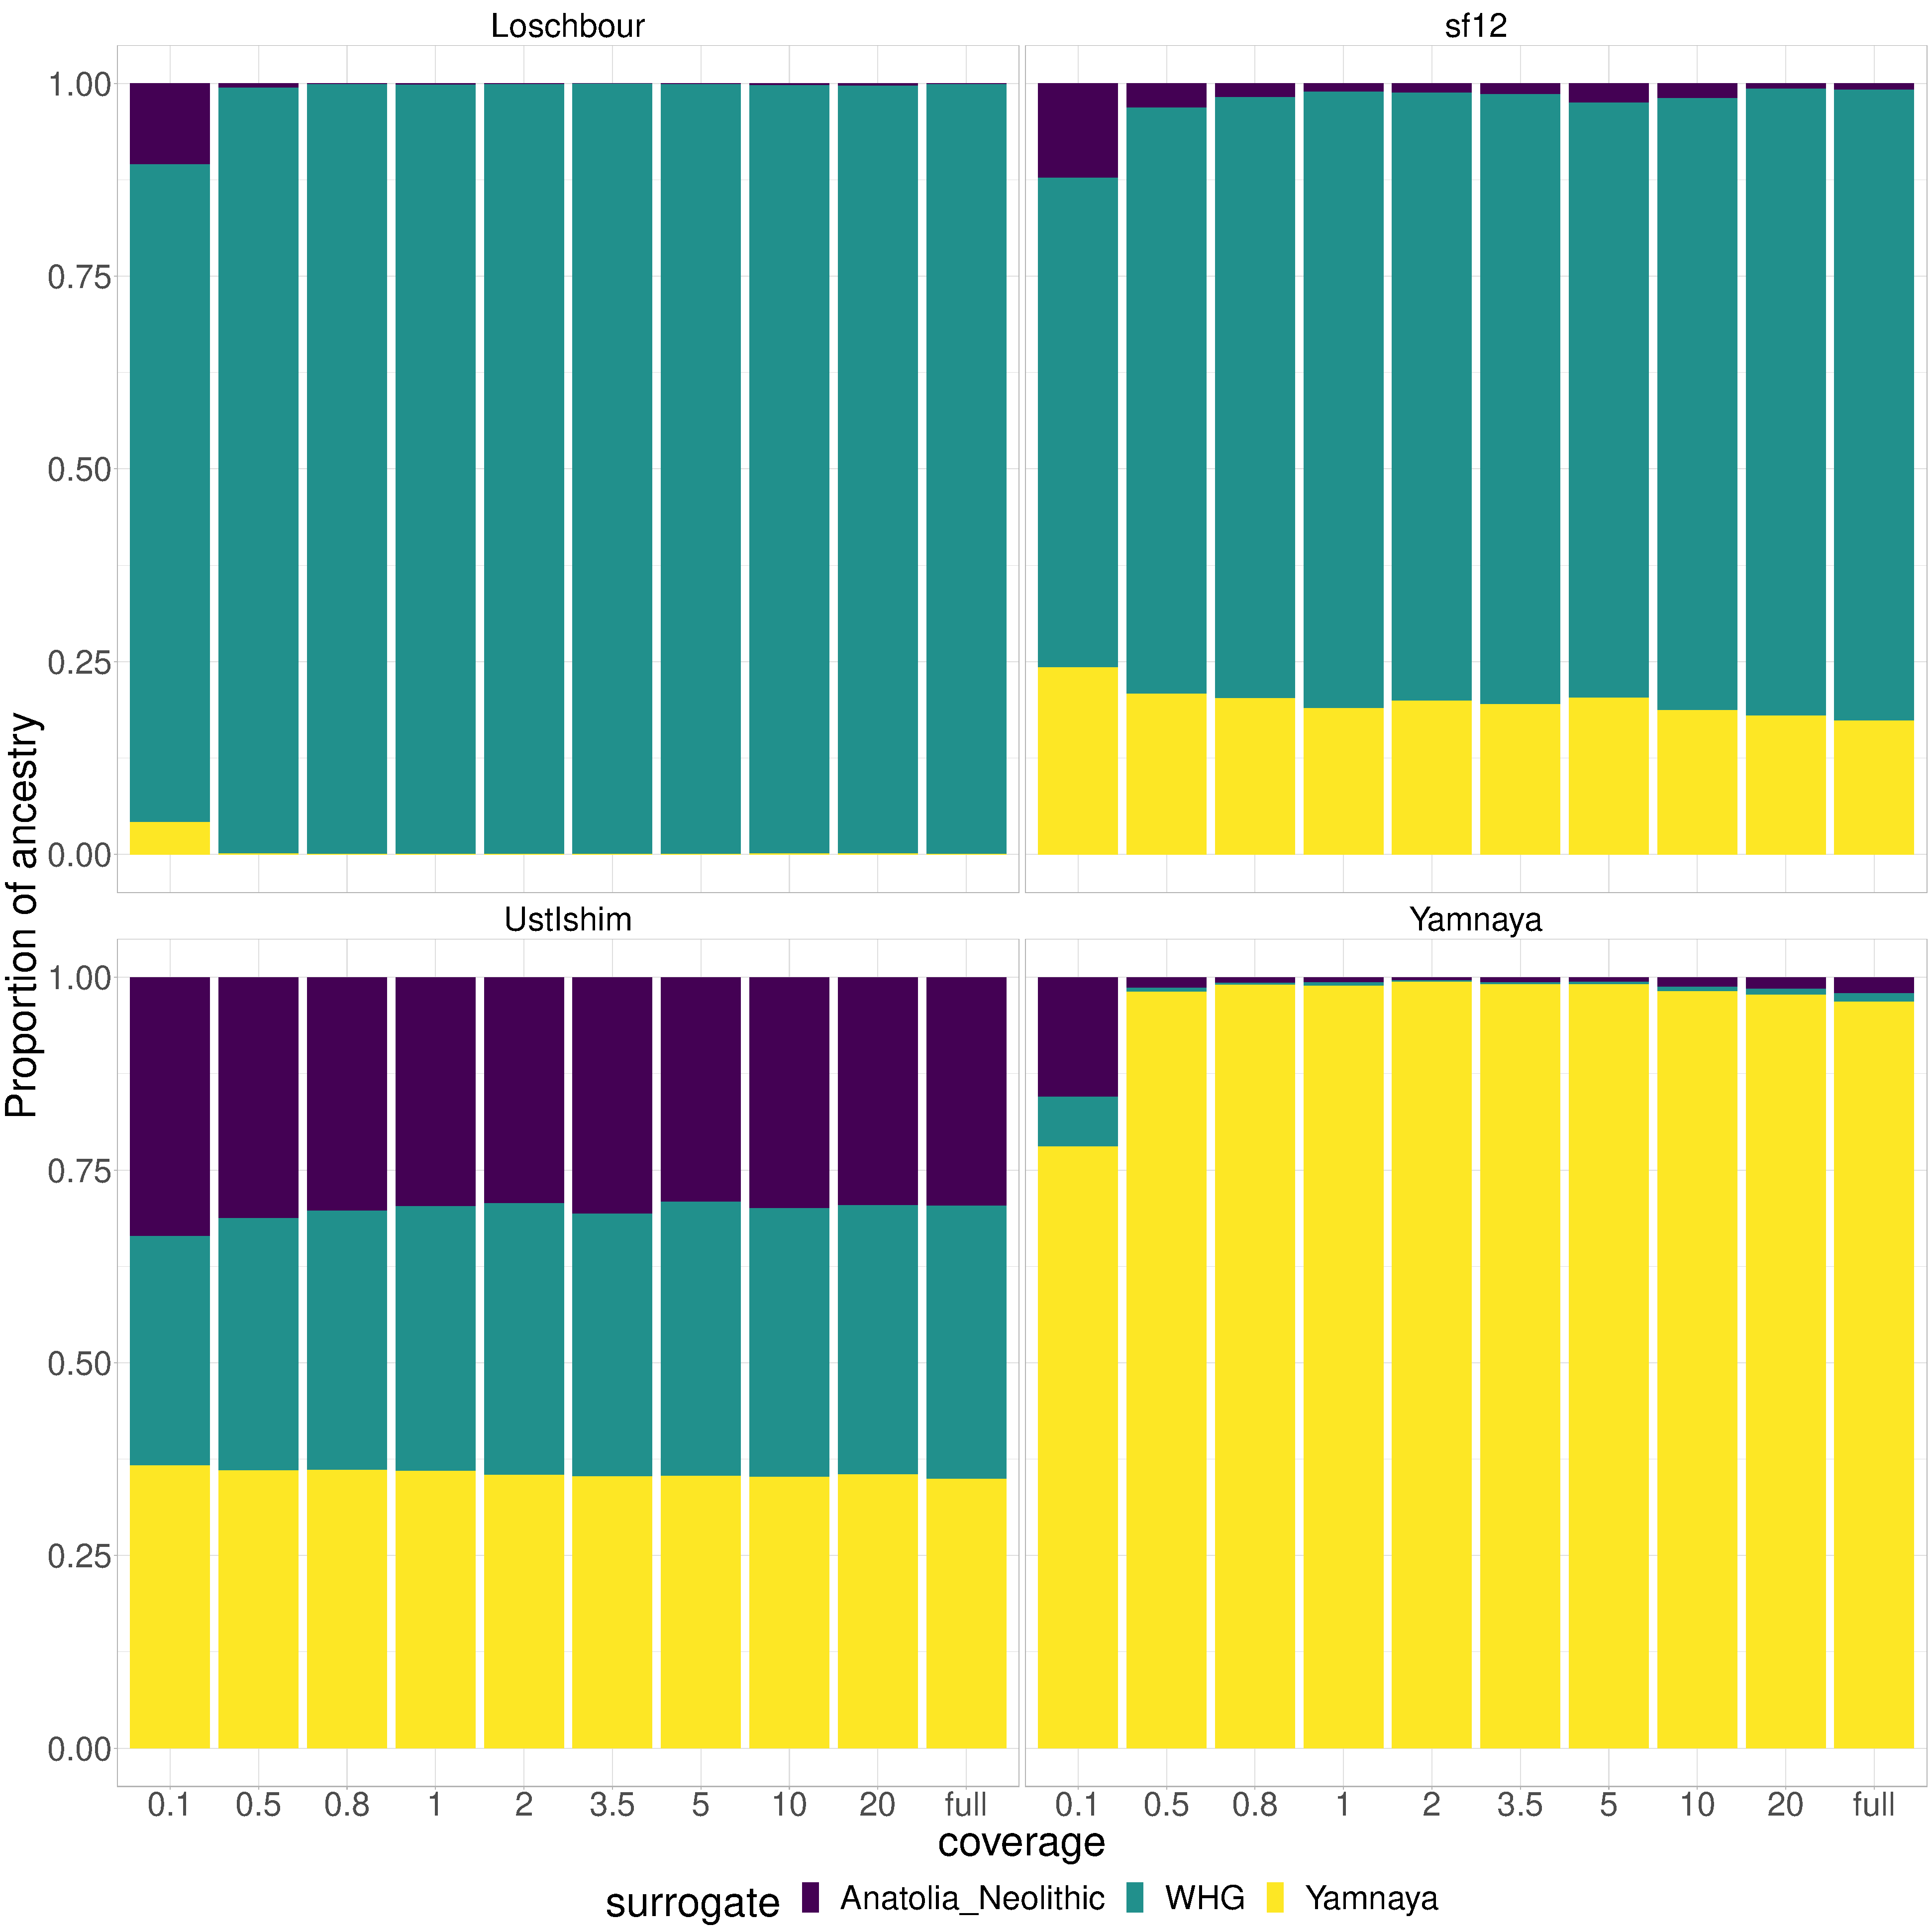
\includegraphics[width=1.0\textwidth]{../images/chapter1/3pop_SF_downsampled.pdf}
    \caption{Each panel gives information for a different downsampled genome. Bars represent proportion of ancestry, coloured by different surrogates. Different coverages for the same individual are given within each panel. 3 surrogates were used.}
    \label{fig:3pop_SF_downsampled}
\end{figure}

The results suggest that SOURCEFIND estimates are robust to coverage effects to 0.5-0.8x coverage. At 0.1x coverage, there is an increase in ancestry components that are not present in higher coverage samples, suggesting they are artifacts caused by low coverage. For example, small components of Anatolia Neolithic and Yamnaya ancestry appear in Loschbour at 0.1x coverage, which are not present at any higher coverages. Above 0.5x coverage, the effect of coverage on estimated ancestry proportions appears to be marginal. For example, in sf12, the different in the minor ancestry component of Anatolia Neolithic is, at most, 2.369\%. 

However, more than 3 surrogates are often used and want to estimate more fine-scale ancestry proportions. I re-ran SOURCEFIND but with a larger number of surrogates (Fig. \ref{fig:SOURCEFIND_AllPSop_downsampled}). 

\begin{figure}[htp]
    \centering
    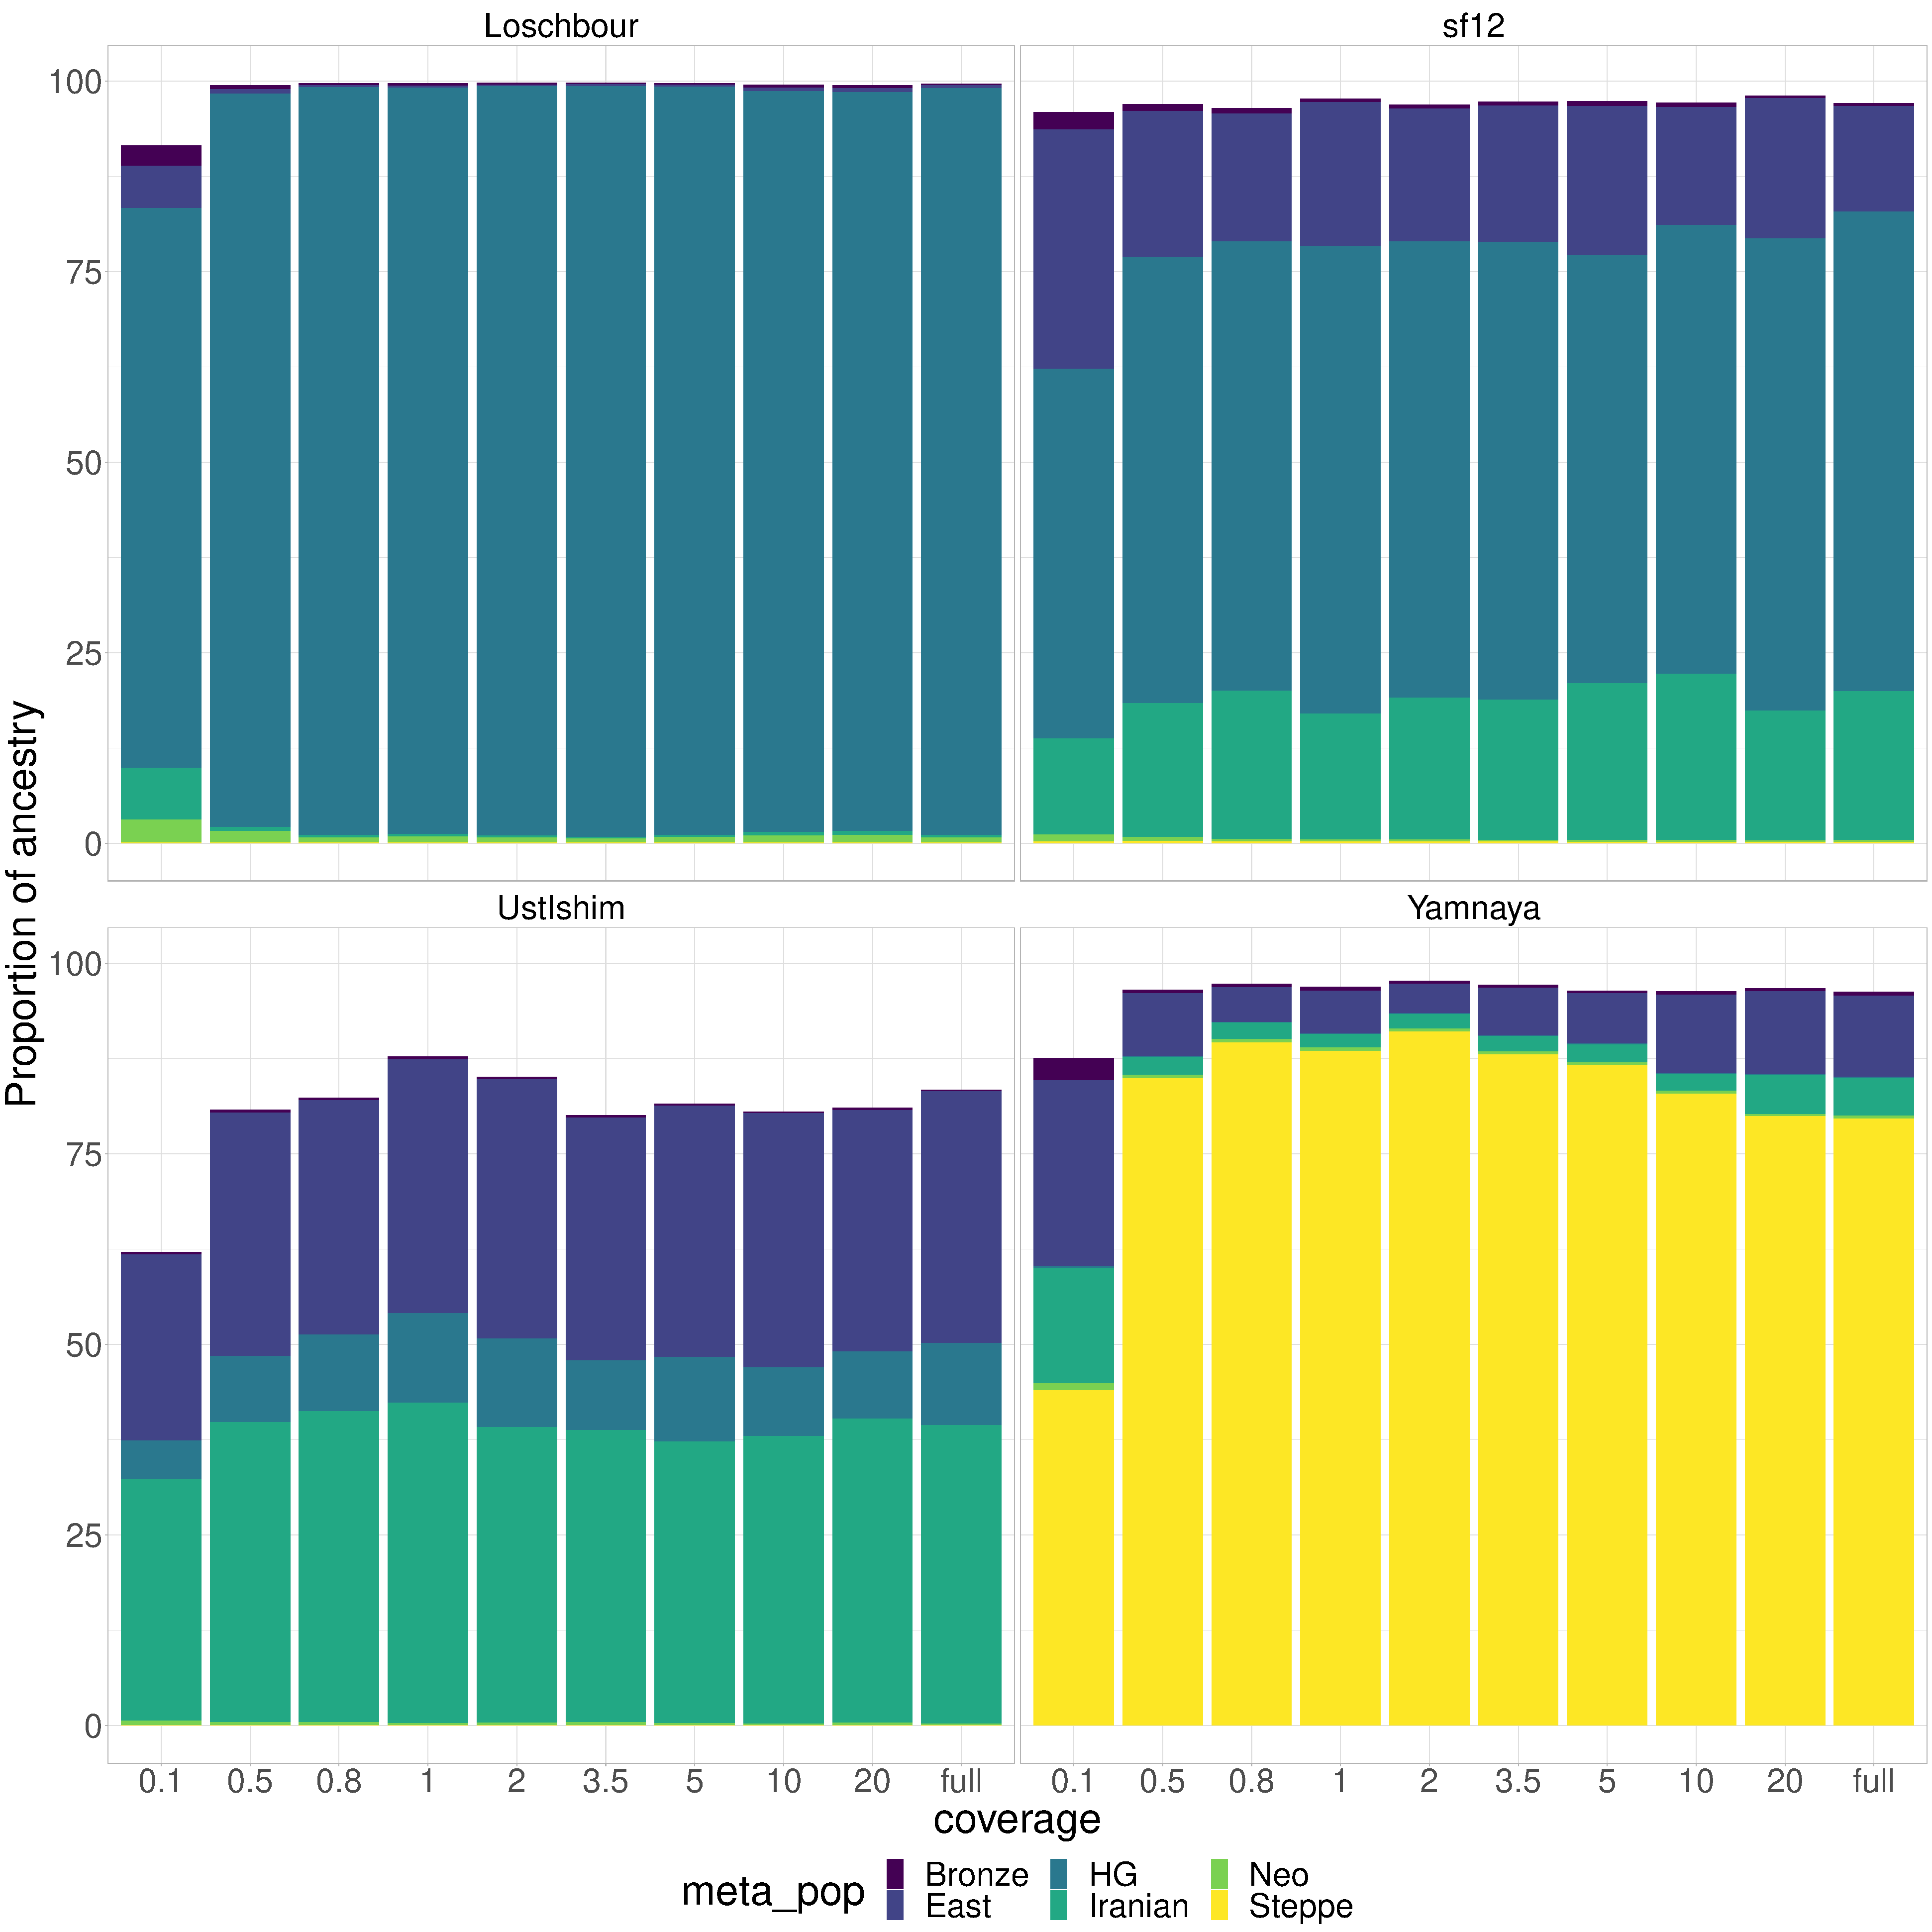
\includegraphics[width=1.0\textwidth]{../images/chapter1/Allpops_SF_downsampled.pdf}
    \caption{Each panel gives information for a different downsampled genome. Bars represent proportion of ancestry, coloured by different surrogates. Different coverages for the same individual are given within each panel. All ancient surrogates were used.}
    \label{fig:SOURCEFIND_AllPSop_downsampled}
\end{figure}

Again, Loschbour seems to be the least affected by coverage, with only slight differences between the 0.5x and full coverage samples. It is known that Upper Paleolithic / Early Neolithic Hunter-Gatherer populations were small and lacked genetic diversity \cite{excoffier1999hunter, Lazaridis2014, Fu2016}. It is therefore expected that Hunter-Gatherers would share longer IBD segments than individuals from outbred populations. Accordingly, this may make estimating SOURCEFIND proportions easier.

I also performed the same analysis but first running ChromoPainter in unlinked mode and using the chunkcounts matrix as the input for SOURCEFIND (Fig \ref{fig:SOURCEFIND_3pop_unlinked_downsampled}). Other than for LBK, these results appear to show that currently, SOURCEFIND is not well calibrated for to estimate ancestry proportions from an unlinked chunkcounts matrix. 

\begin{figure}[htp]
    \centering
    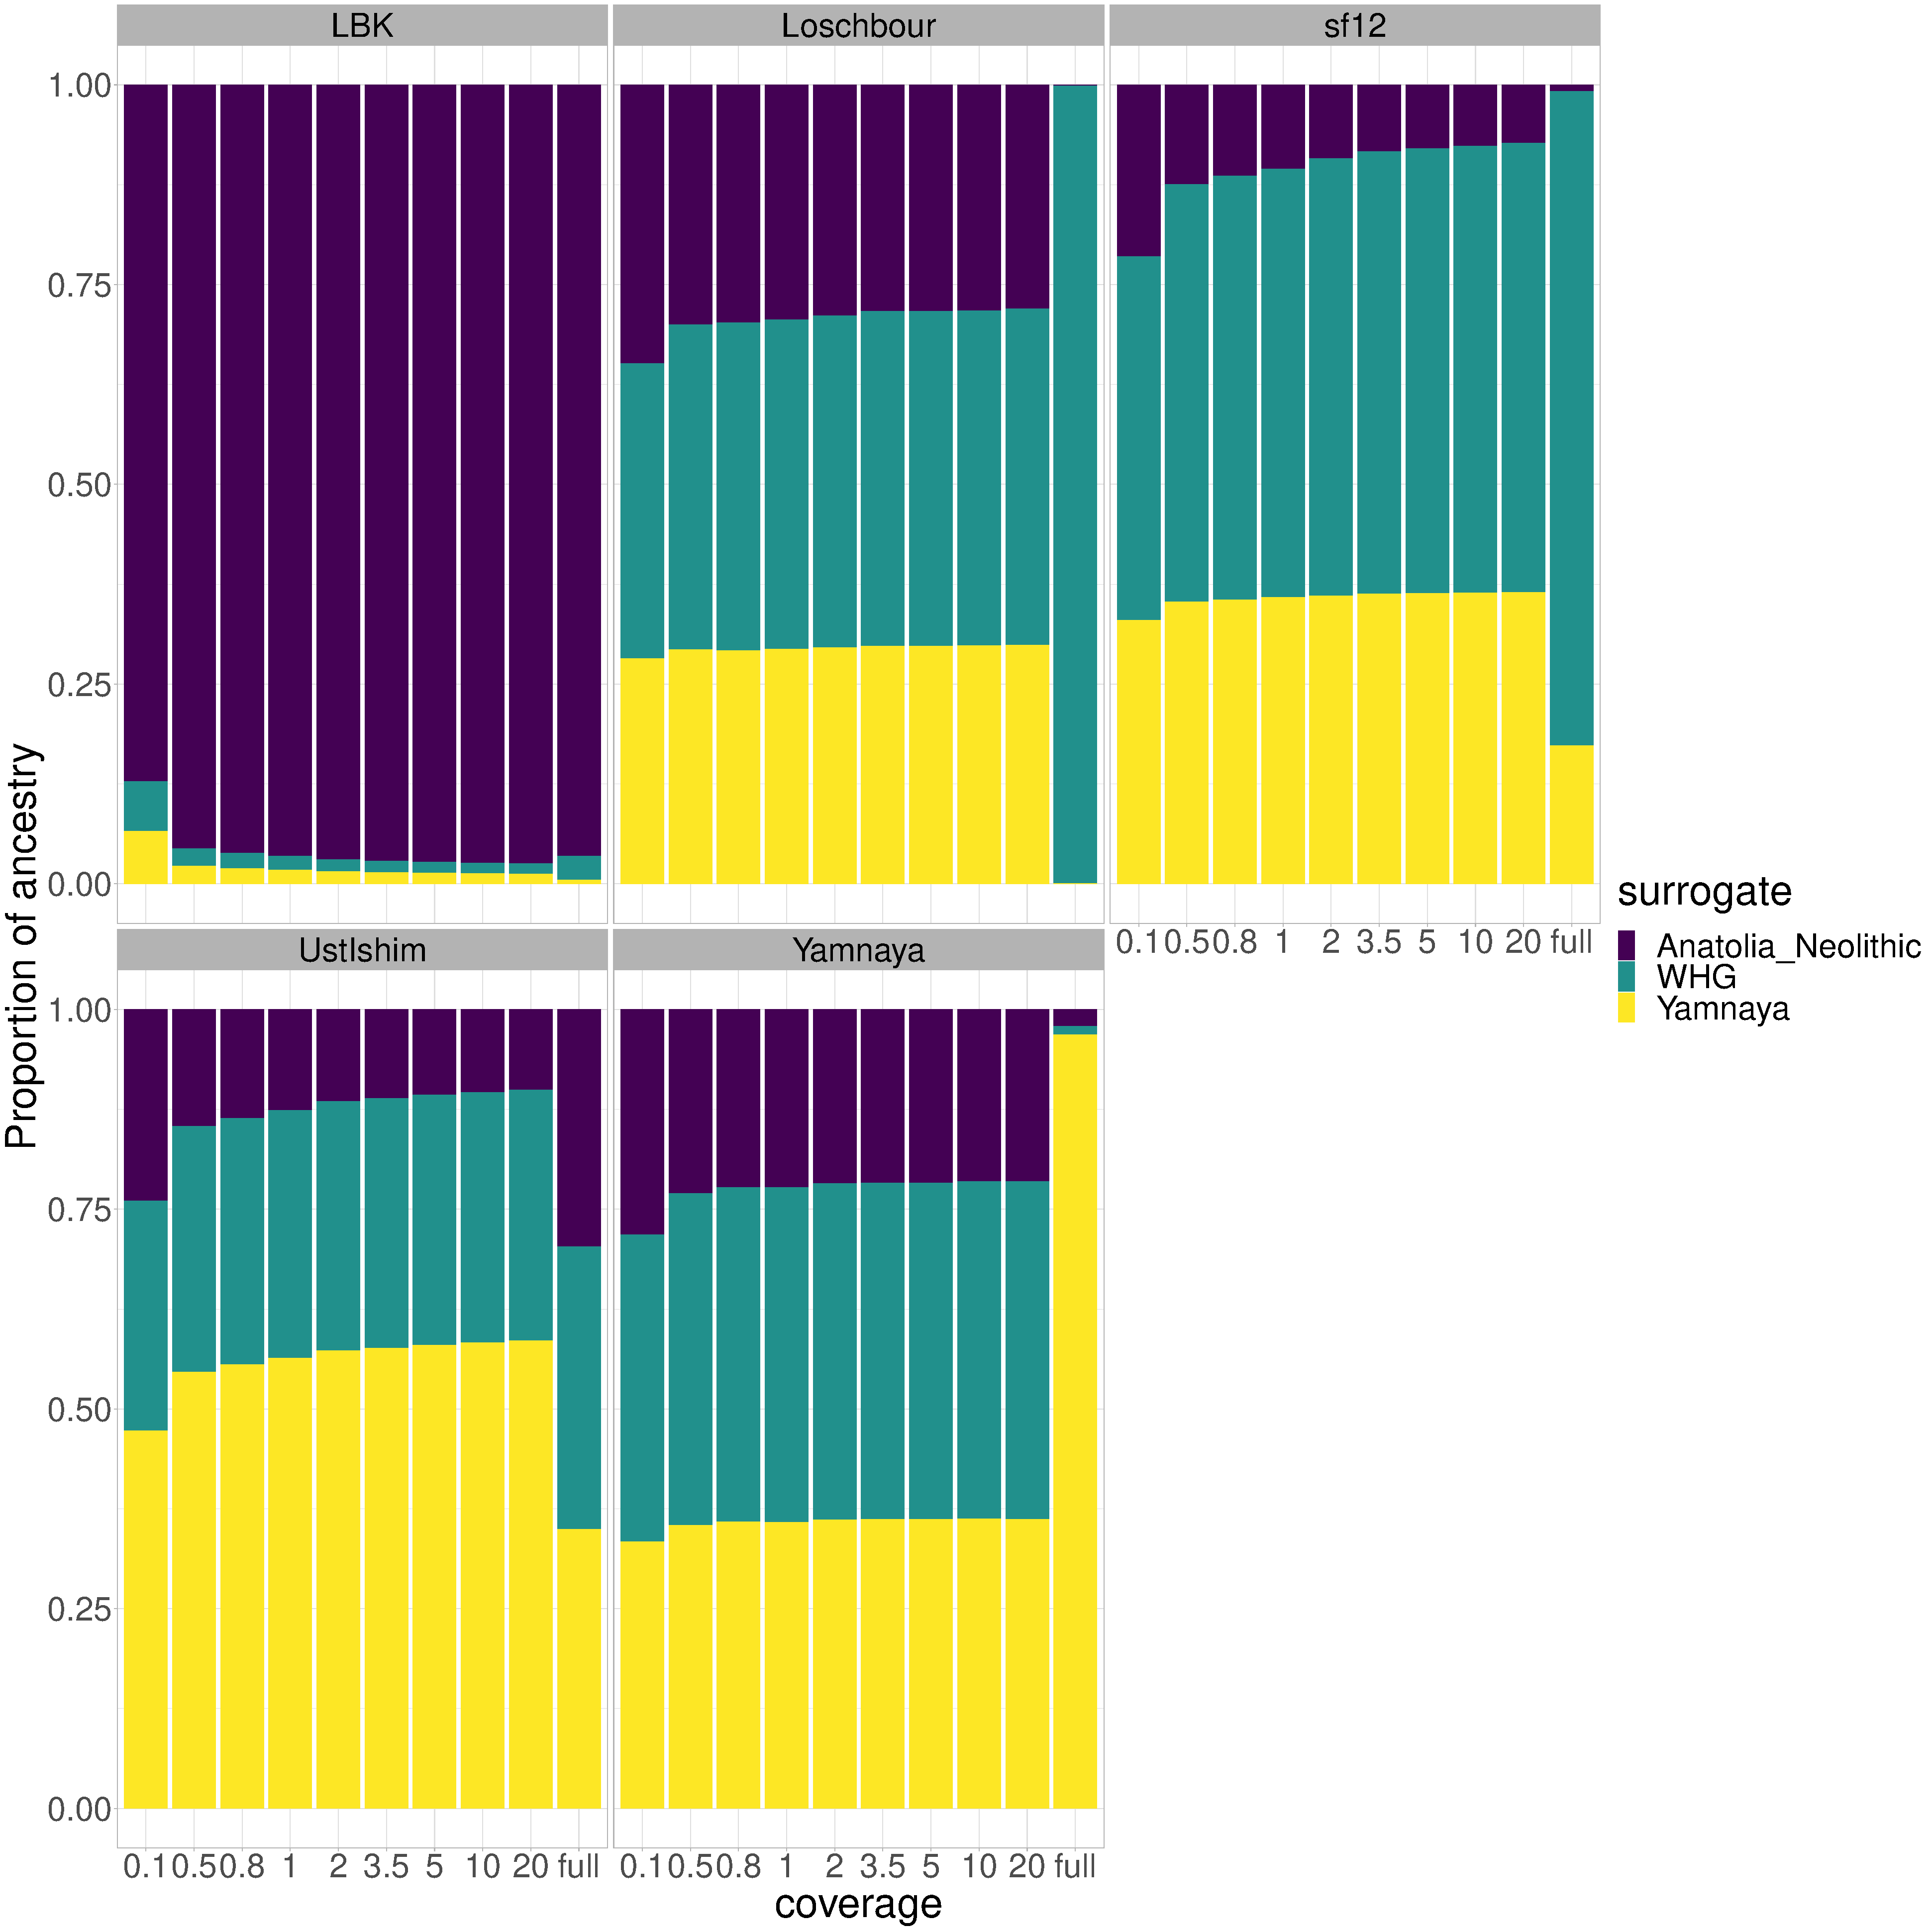
\includegraphics[width=1.0\textwidth]{../images/chapter1/3pop_SF_downsampled_unlinked.pdf}
    \caption{Each panel gives information for a different downsampled genome. Bars represent proportion of ancestry, coloured by different surrogates, generated from the unlinked chunklengths matrix. Different coverages for the same individual are given within each panel. 3 surrogates were used.}
    \label{fig:SOURCEFIND_3pop_unlinked_downsampled}
\end{figure}

\section{Issues and possible solutions for low coverage ancient DNA}

The previous section detailed some of the drawbacks of performing ChromoPainter analysis on low coverage ($<$0.5x) ancient DNA samples. , reducing the sequencing coverage of ancient DNA samples has the effect of pulling each sample towards origin of a principle component analysis (PCA) relative to the same sample at higher coverage (Fig. \ref{fig:PCA_panel_allInds_allCoverage}). This is evident for the lowest coverage samples at 0.1x. 

This section will therefore consider mitigation strategies. However, first it is necessary to elucidate the potential causes of this coverage related bias. 

\subsection{Causes}

This section will consider the possible causes of the observed phenomena of low coverage samples being pulled towards the centre of the PCA. First, it is necessary to outline the possible effects of low-coverage on genotype calling and phasing. 

\subsubsection{Phasing bias / switch errors}

Phasing relies on having a reference panel of individuals from whom it is possible to reconstruct the the haplotypes of a target individual from. A 'switch-error' occurs when an individual incorrectly switches from copying from the correct to an incorrect reference haplotype, or in effect false recombination events which occur between the inferred haplotypes compared with the true haplotypes \cite{choi2018comparison}. Previous research has shown that reduced coverage results in an increase in the number of switch errors, presumably because of the increased chance of incorrectly called genotypes at lower coverage \cite{rubinacci2021efficient}. Therefore, one potential cause of low coverage samples moving towards the origin of the PCA could be an increase in switch errors caused by an increase in genotyping errors. For example, a switch error may arise when a true heterozygous position is incorrectly called as a homozygous position due to low coverage, and the correct allele on one of the haplotypes cannot be phased. 

The possible effect of increased switch errors at lower coverage can be testing by running ChromoPainter under the unlinked model, which assumes a model of linkage equilibrium between neighbouring SNPs and essentially regresses to a model of allele frequency differences \cite{Lawson2012}. Thus, switch errors / incorrectly phased heterozygous positions would not be expected to influence the painting under the unlinked model. To test the potential effect of phasing  bias / switch errors, I performed the same painting as in Fig. \ref{fig:PCA_panel_allInds_unlinked.allCoverage}, but in unlinked mode. 

\begin{figure}[htp]
    \centering
    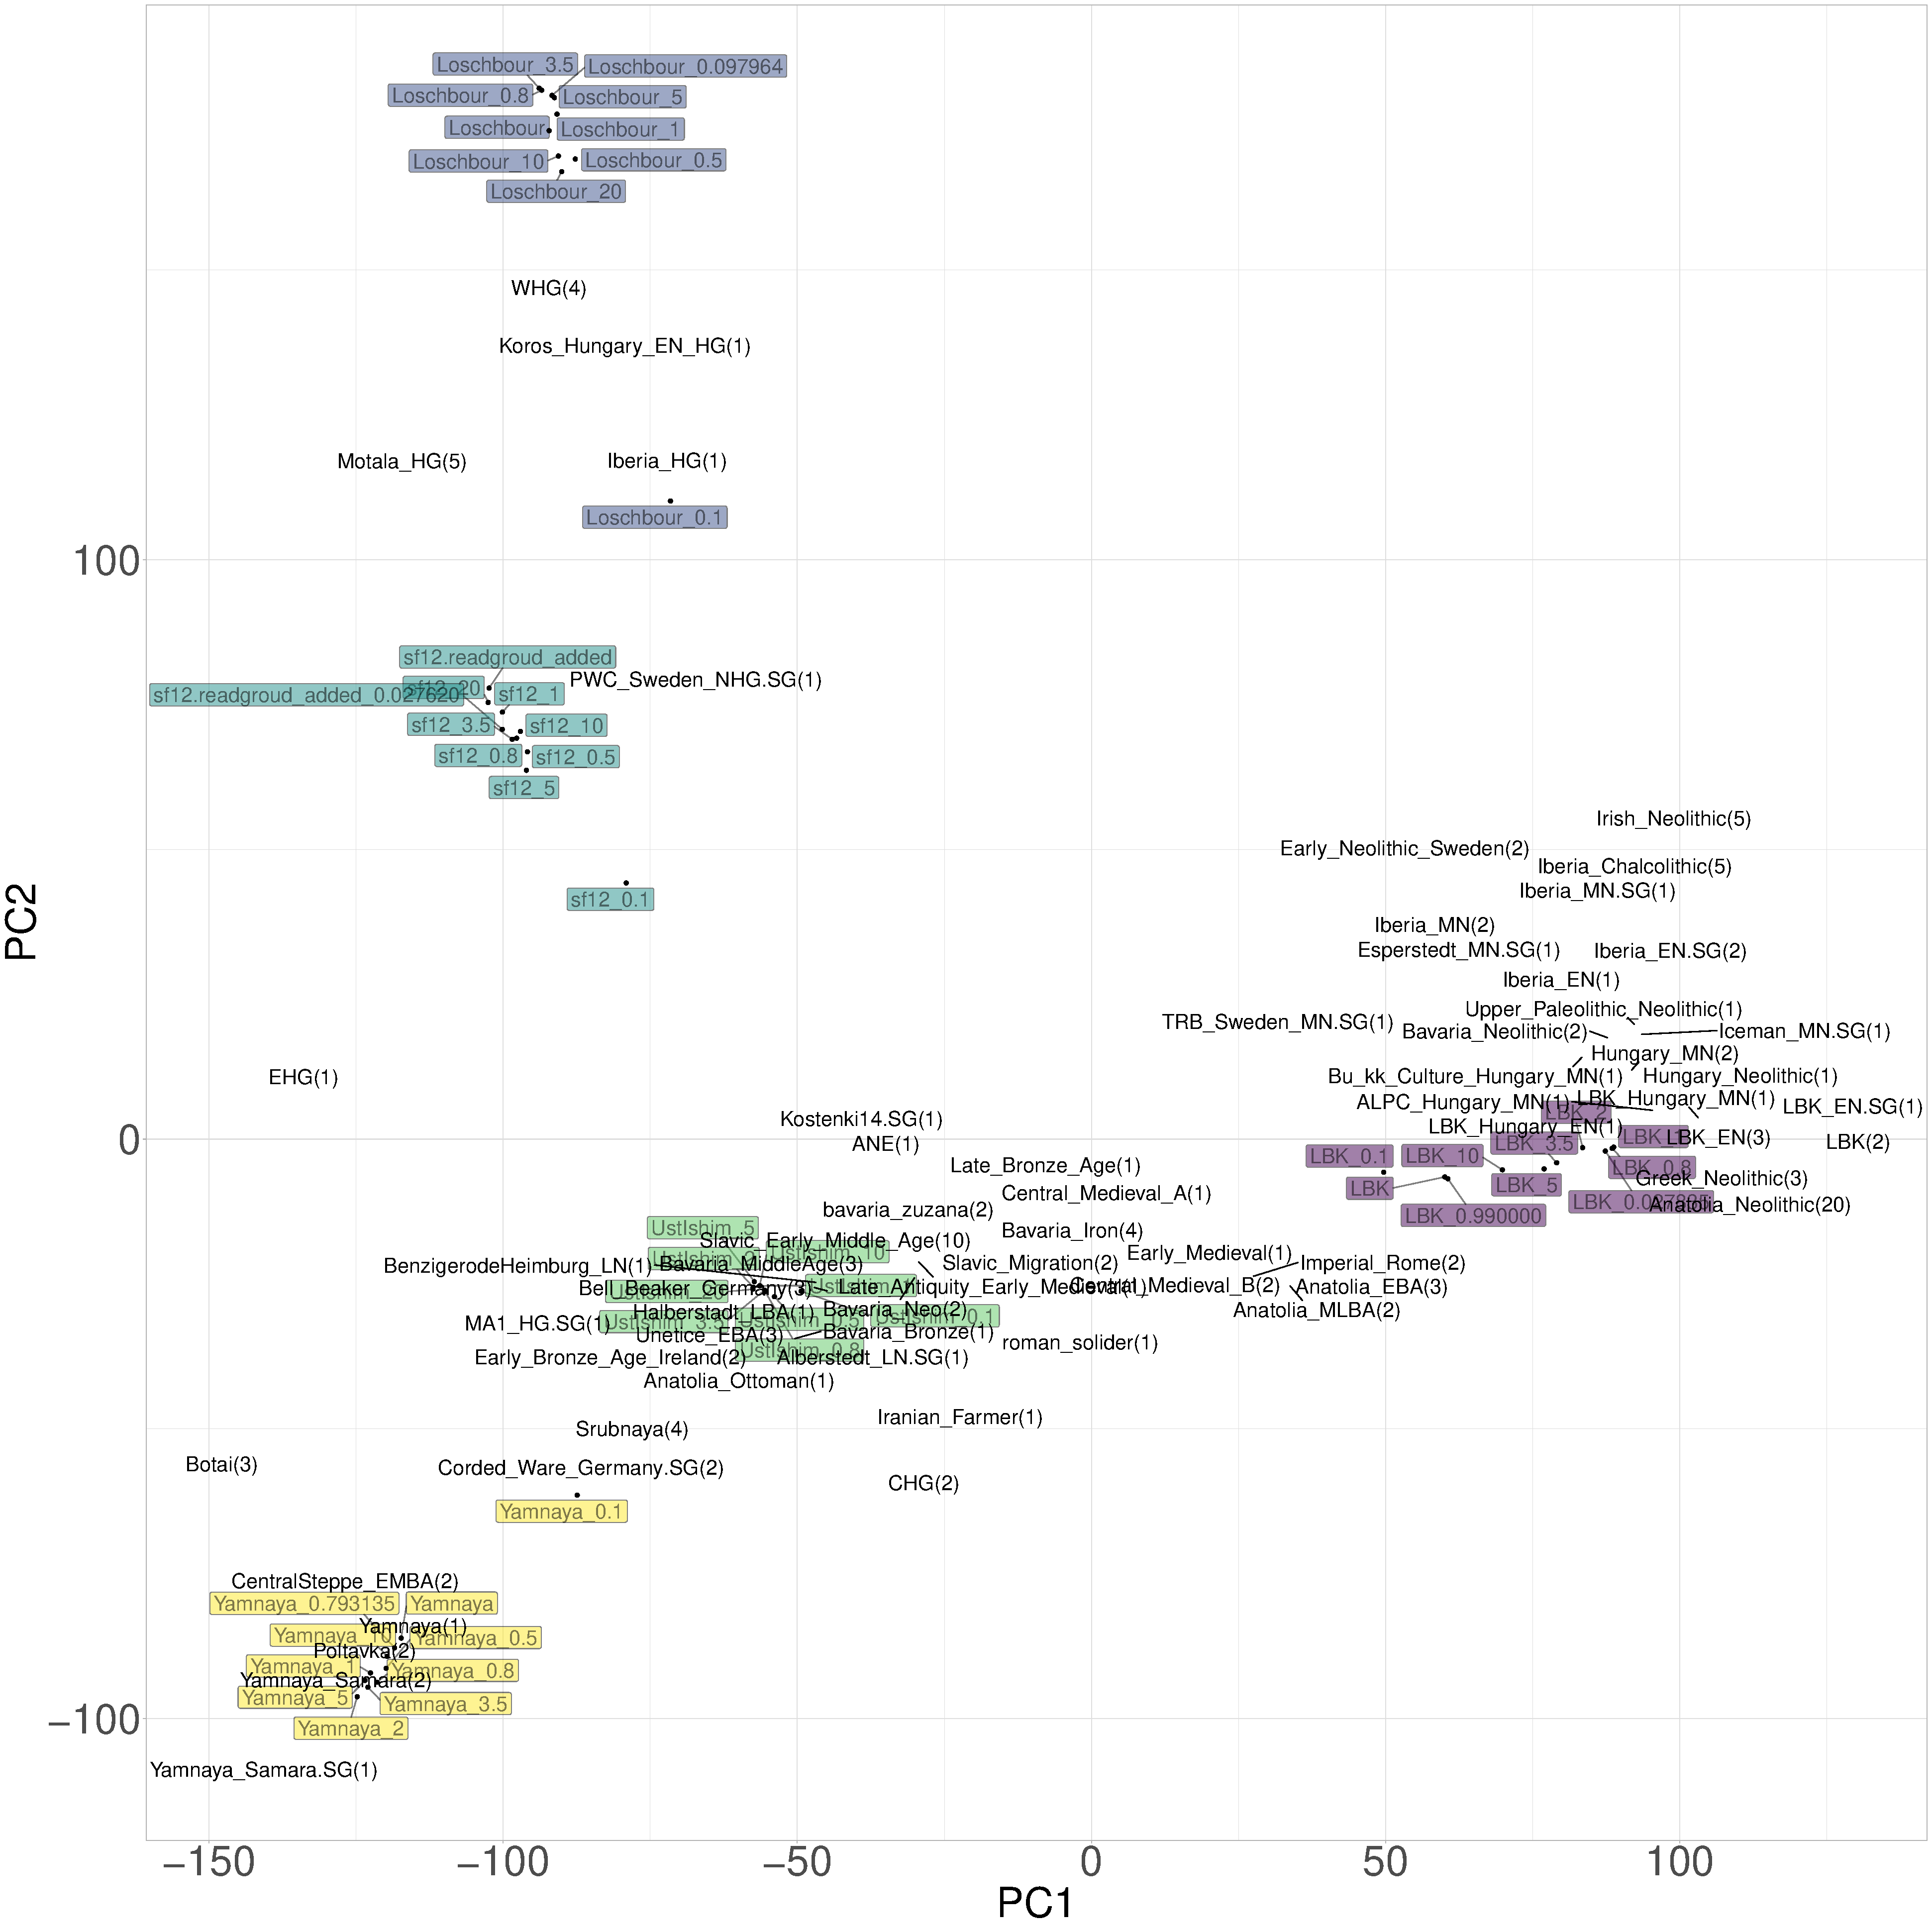
\includegraphics[width=1.0\textwidth]{../images/chapter1/PCA_panel_allInds_unlinked.allCoverage.pdf}
    \caption{Principle component analysis (PCA) of downsampled, full coverage and reference ancient individuals generated from the unlinked chunklengths matrix. Full coverage and downsampled genomes of the same individual are coloured the same. Reference individuals are grouped into populations plotted as the mean principle components for all individuals within the population.}
    \label{fig:PCA_panel_allInds_unlinked.allCoverage}
\end{figure}

Fig. \ref{fig:PCA_panel_allInds_unlinked.allCoverage} shows the same PCA, but on the chunkcounts matrix from the corresponding unlinked painting (because 'chunks' are formed from linked SNPs, there is no lengths matrix output from the unlinked model - the equivalent is the counts matrix). It is clear that the same issue persists and that lower coverage individuals are still pulled towards the centre of the PCA, suggesting that phasing switch errors are not the main issue. It is also clear that much of the population structure (e.g. the ability to separate the Neolithic and Bronze Age clusters) disappears when using the unlinked painting. 

\subsection{Imputation bias}

The previous section indicated that phasing issues are no the primary cause of coverage-related bias.

One other possible cause could be the tendency to incorrectly assign genotypes as homozygous when they are in fact heterozygous. This is because when a true heterozygous genotype is covered by a low number (e.g. 1 or 2) reads, there is a higher probability that there are no reads sampling one of the alleles. For example, if we assume that there is an equal probability of a read sampling either allele, then if the position is only covered by a single read, there is a 50\% chance one of the alleles would not be sampled and the genotype would be incorrectly assigned as a homozygous. Even when there are 5 reads covering a position, there is still 3.125\% chance that one of the alleles would not be sampled by a read. Because homozygous genotypes do not need to be phased, these errors would not be mitigated by running ChromoPainter in unlinked mode.

\subsection{Explicit test of cause}

To test the explicit cause of the coverage-related bias, I removed different sets of SNPs from downsampled individuals. I took the phased haplotypes for all 5 individuals downsampled to 0.1x and 0.5x and compared them to the same individuals at full coverage. Positions were classified as different kinds of mismatch between the downsampled and full coverage individual; a) dosage mismatch if the dosage differed, b) 'hap-A' mismatch if the alleles on the first haplotype differed, c) 'hap-B' mismatch if the alleles on the second haplotype differed and d) 'hap-a-hap-b' mismatch if the alleles on the first and second haplotypes differed. 

NB: I am waiting for this to finish so don't have the results yet. 

\section{Solutions}

In this section I will explore several potential solutions to the issue of coverage-related bias.

\subsection{Accounting for allele likelihoods}

Section 2.2.1 describes a novel improvement to the ChromoPainter algorithm. Briefly, instead of assuming that each allele along a haplotype is correct with a probability 1 $-$ $\theta$, where $\theta$ represents a generic error probability, the posterior genotype probability from GLIMPSE is accounted for in the emission probabilities of the copying model. The motivation behind this improvement is that the uncertainty associated with genotype calls at low coverage is suitably propagated throughout the painting process, resulting in uncertain alleles contributing less towards the expected copying values than more certain ones.  


\subsection{Filtering SNPs}

Here I will test whether filtering the set of input SNPs on different criteria reduces the effect of coverage related bias. 

The frequency of a particular variant in the reference panel (RAF - reference allele frequency) used for imputation is know to affect how accurately that variant can be imputed. Specifically, we expect variants which are less frequent in the reference panel to be imputed at a lower accuracy than those which are more frequent. Therefore, removing variants with a low frequency in the reference panel may mitigate the coverage related bias by removing variants which have been incorrectly imputed. In other words, we want to retain the SNPs were both alleles are relatively common within the population. 

I took the 428,425 SNPs retained form the HellBus set and removed SNPs with $0.1 < RAF > 0.9$, removing a total of 50,187 SNPs. I painted individuals downsampled to 0.1x and 0.5x using the standard set of 125 ancient donor individuals. 

Comparing the r-squared and visually inspecting the relationship between the copvectors showed that this did not improve the 0.5x copyvectors (Fig.  \ref{fig:CP_correlation_allSamples_0.1x_0.5x_30x.RAF_filter}.


\begin{figure}[htp]
    \centering
    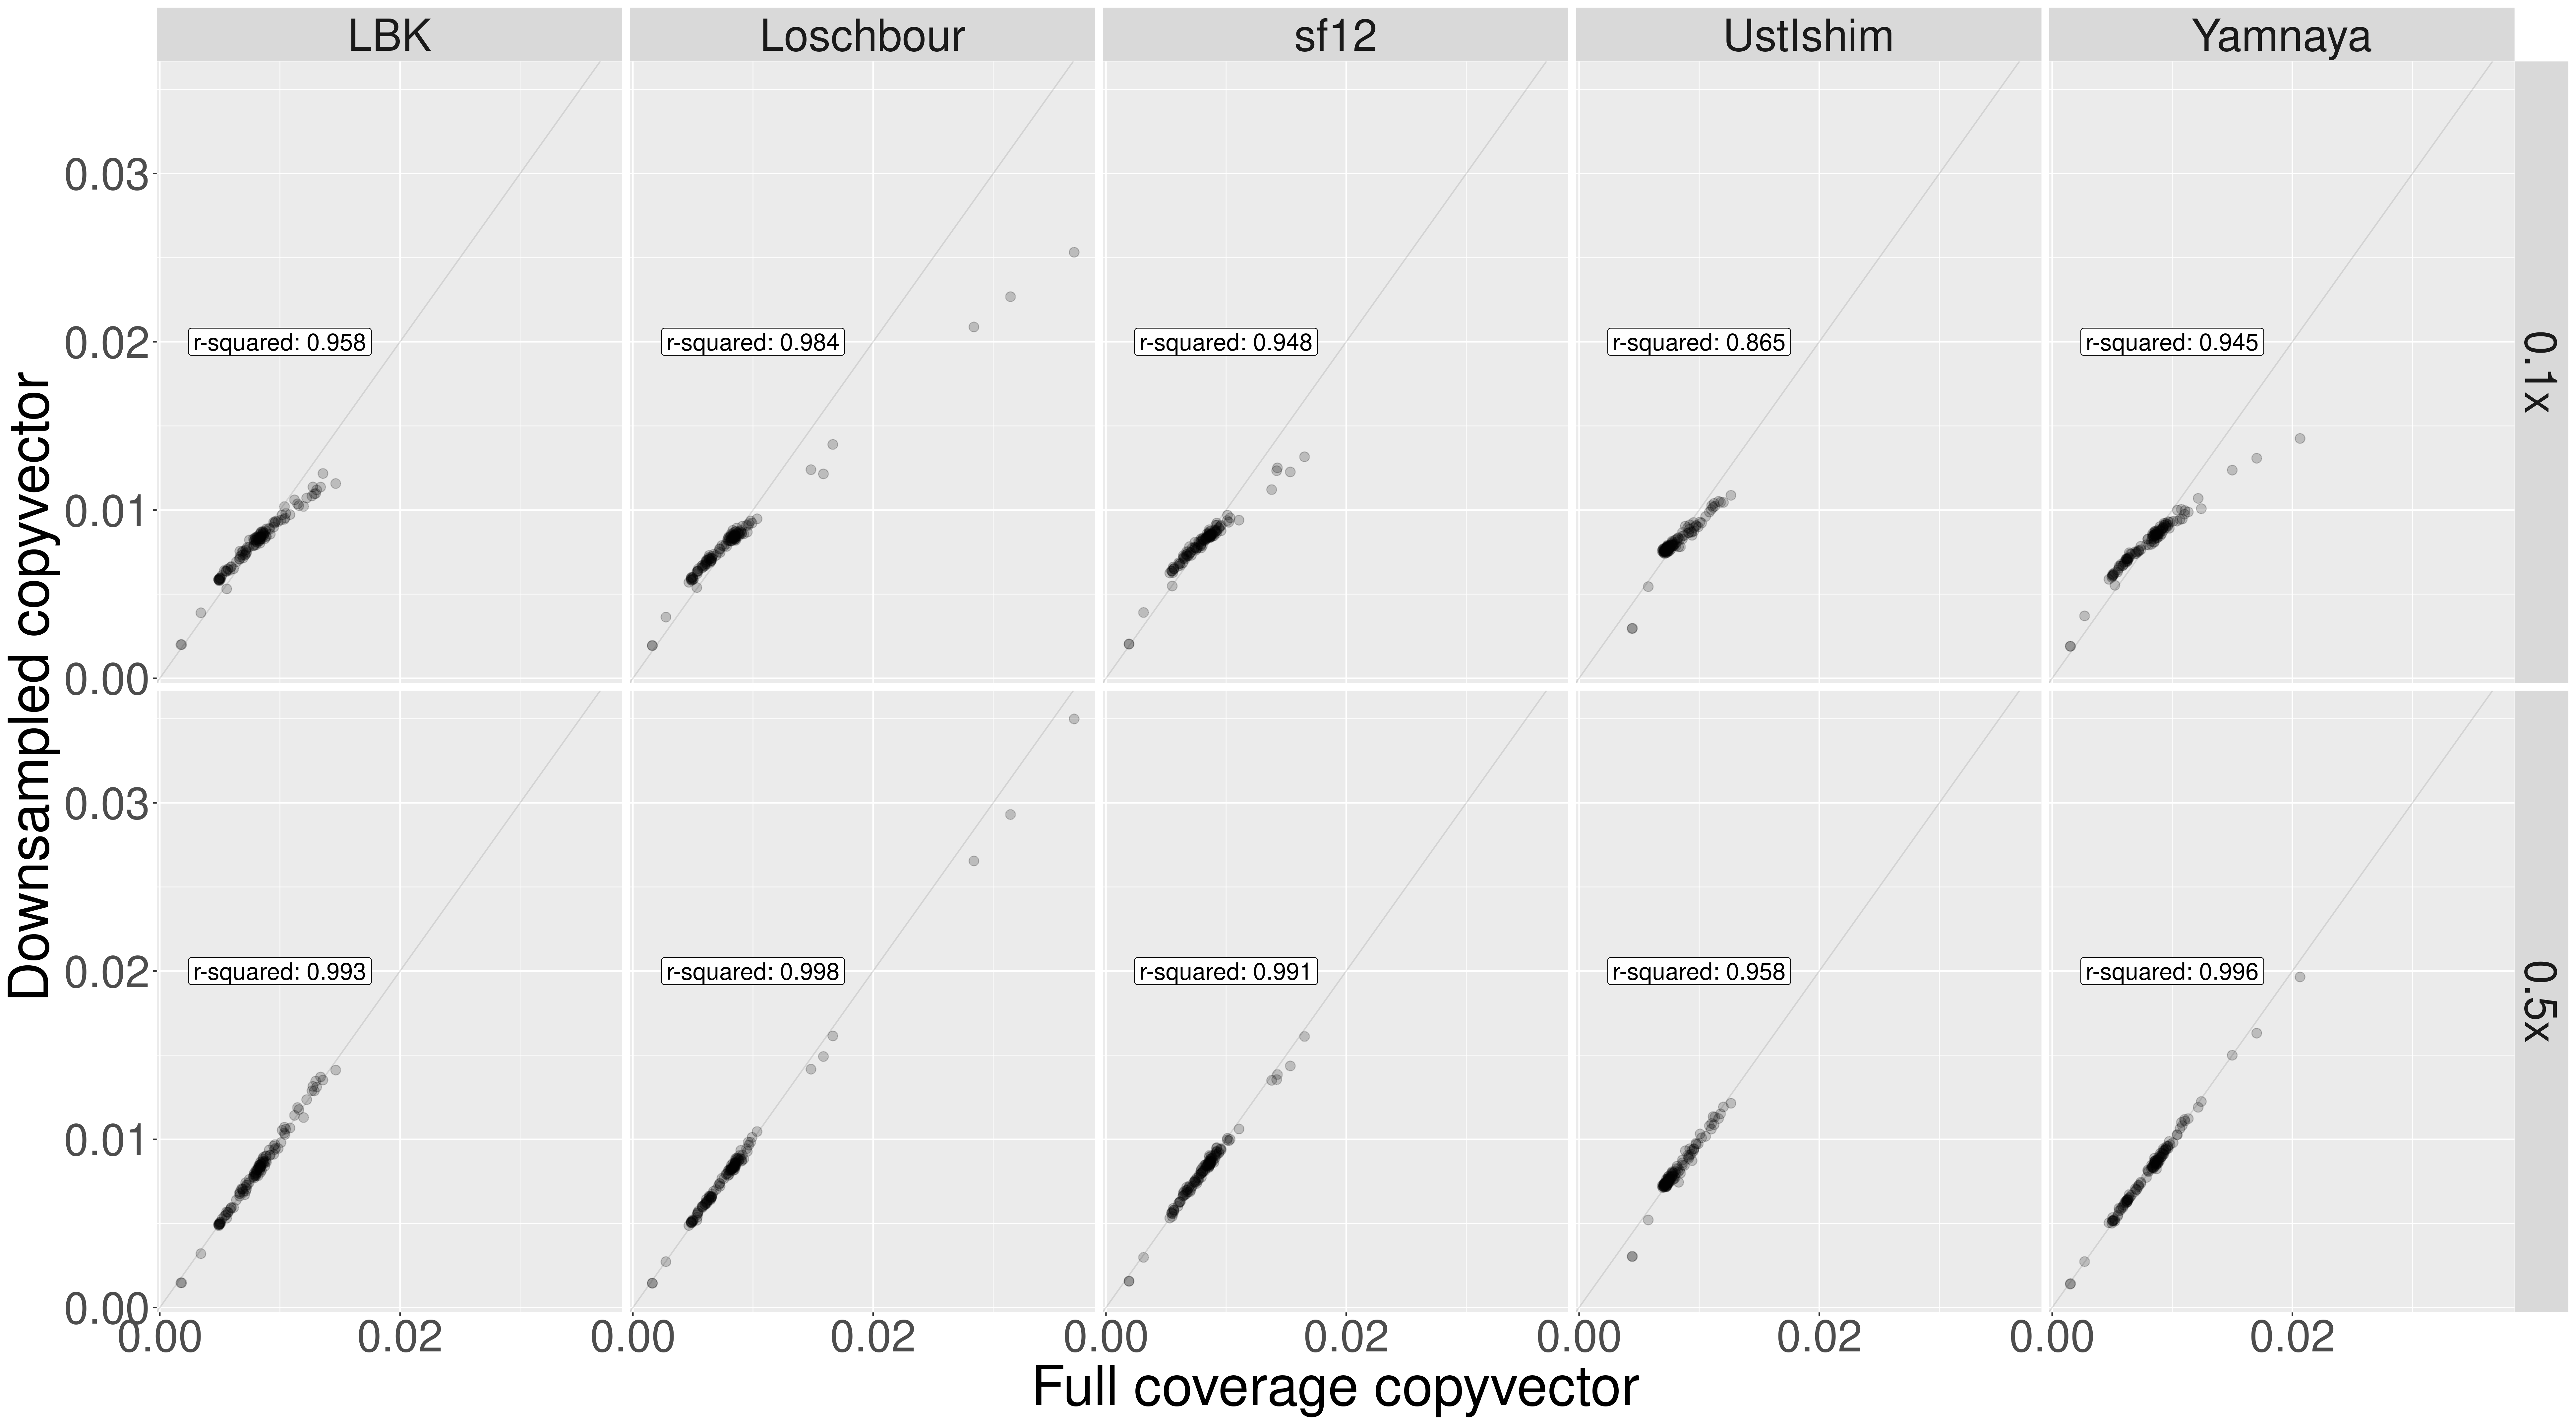
\includegraphics[width=1.0\textwidth]{../images/chapter1/CP_correlation_allSamples_0.1x_0.5x_30x.RAF_filter.png}
    \caption{R-squared between downsampled and full coverage copyvectors when filtering out sites with $0.1 < RAF > 0.9$ at 0.1x coverage (L) and 0.5 coverage (R).}
    \label{fig:CP_correlation_allSamples_0.1x_0.5x_30x.RAF_filter}
\end{figure}
 
I then chose to filter SNPs based on $max(GP)$ at each position. For each individual downsampled to 0.5x, I only retained positions where the $max(GP) >= 0.990$. This resulted in a total of 348,852 SNPs for LBK, 339,949 for Loschbour, 315,075 for sf12, 308,961 for UstIshim and 386,484 for Yamnaya. Because different SNPs were removed from different individuals, each individual was painted separately. The same standard set of 124 ancient donors was used. 

Again, this did not improve the accuracy of the copyvectors (Fig. \ref{fig:CP_correlation_allSamples_0.1x_0.5x_30x.GP_filter}).

\begin{figure}[htp]
    \centering
    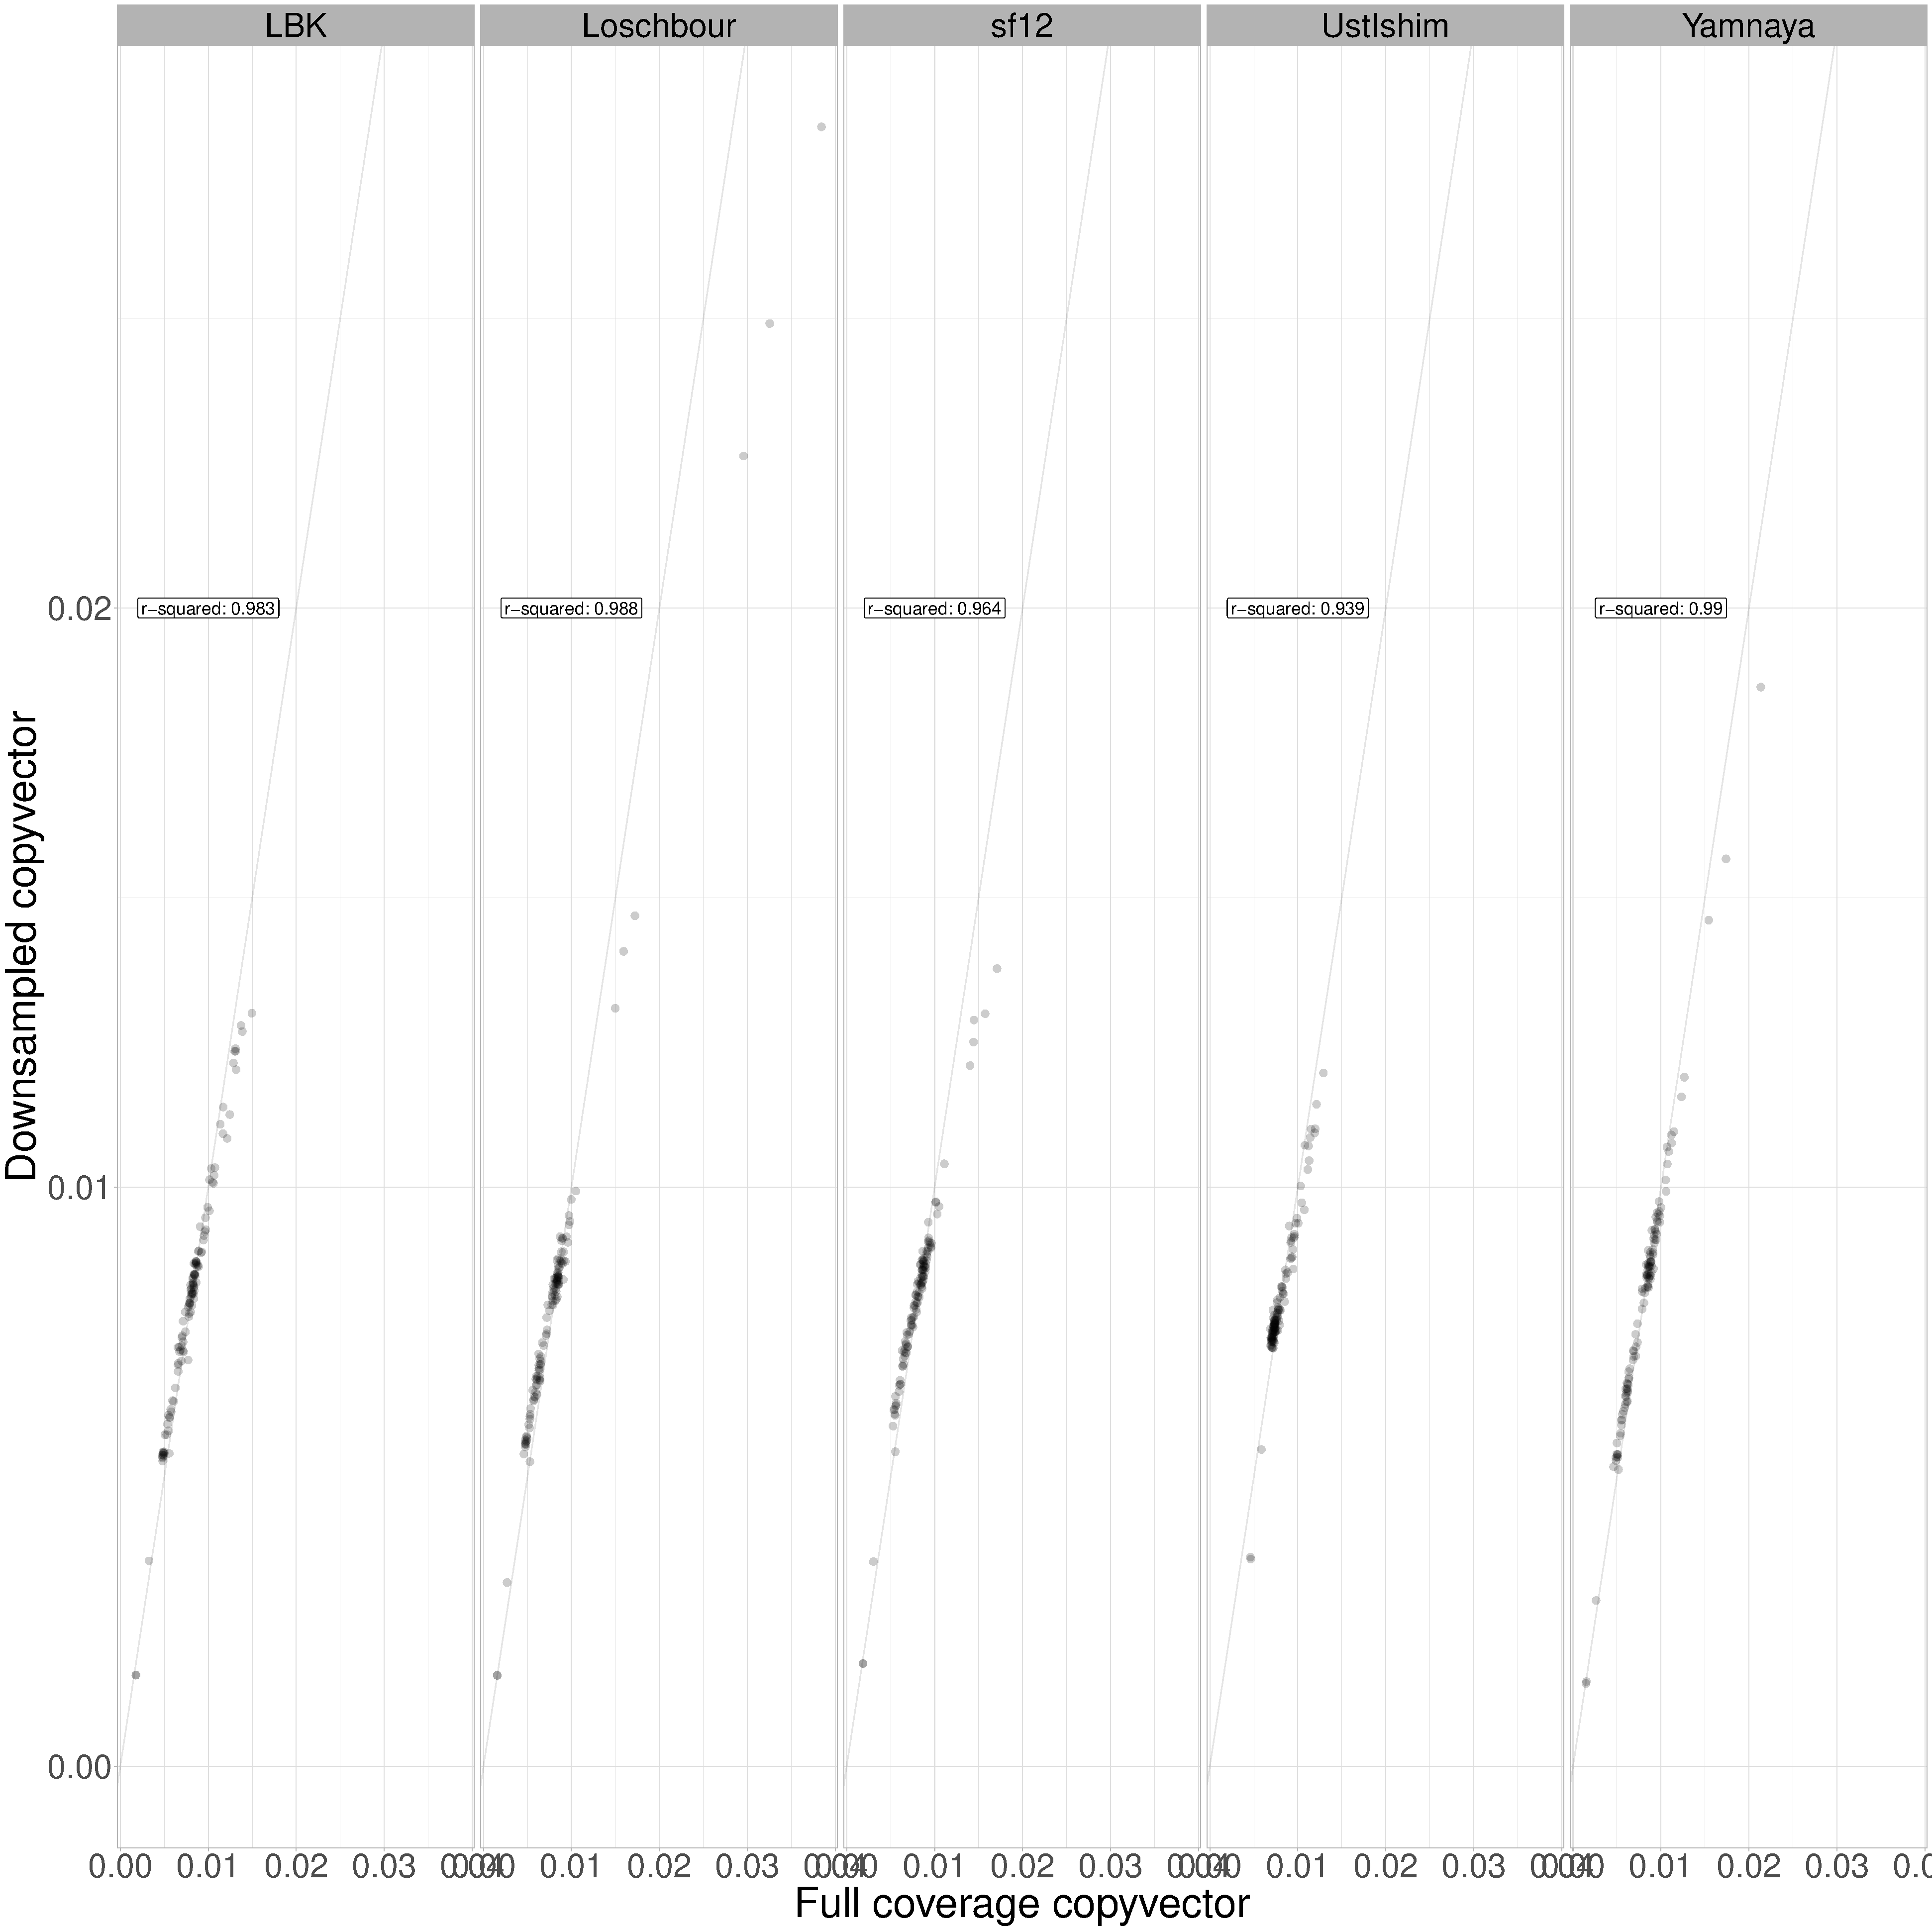
\includegraphics[width=1.0\textwidth]{../images/chapter1/CP_correlation_allSamples_0.1x_0.5x_30x.GP_filter.pdf}
    \caption{R-squared between downsampled and full coverage copyvectors when filtering out sites with $max(GP) >= 0.990$ at 0.1x coverage (L) and 0.5 coverage (R).}
    \label{fig:CP_correlation_allSamples_0.1x_0.5x_30x.GP_filter}
\end{figure}


\subsection{Upweighting densely genotype regions of high coverage}

The previous section showed that imputation error was likely the cause of coverage related bias in low coverage samples. Therefore, excluding SNPs which have been imputed, or restricting the painting to non-imputed SNPs above a certain coverage may help to mitigate coverage-related bias.

This would result in painting a set of SNPs which is necessarily a) smaller and b) less dense than the original set of SNPs. Reducing either then total number of density of SNPs may reduce the accuracy / increase the noise of estimated copvectors. Therefore, it is necessary to establish this effect. In particular, we would like to know what is the minimum number and density of SNPs needed to retain useful haplotype information and the advantages of haplotype-based methods over unlinked methods. 

One way to test this is to utilise previous results which showed it is possible to distinguish between individuals sampled from Devon and Cornwall using haplotype-based methods (e.g. ChromoPainter and the fineSTRUCTURE algorithm), but not unlinked methods (ADMIXTURE \cite{alexander2009fast}) \cite{Leslie2015}. Leslie et al (2015) identified structure between individuals from Devon and Cornwall via fineSTRUCTURE groupings. However, repeating the fineSTRUCTURE from Leslie et al is time consuming, and similar conclusions can be drawn from considering the aggregated amount individuals from Devon and Cornwall copy from their own populations.

The effect of reducing the number of SNPs on the estimated copyvectors of individuals from Cornwall is visualised in Fig. \ref{fig:Devon_Cornwall_copyvectors_sample_size_reduced}. At the lowest level of reducing SNPs (0.002 on the figure), the black points, representing the mean amount individuals from that population copy from the particular donor population, exactly align with the red points, which represent the sample size for that donor population. Therefore, at this number of SNPs, there is almost no information in the copyvectors and the values simply reflect the sample size of the donor group. Accordingly, the copyvectors at this level regress to the prior, where the prior is the sample size of the donor group. On the other hand, at the highest level of reducing SNPs (0.9 on the figure), the black points no longer align with the red points. 

\begin{figure}[htp]
    \centering
    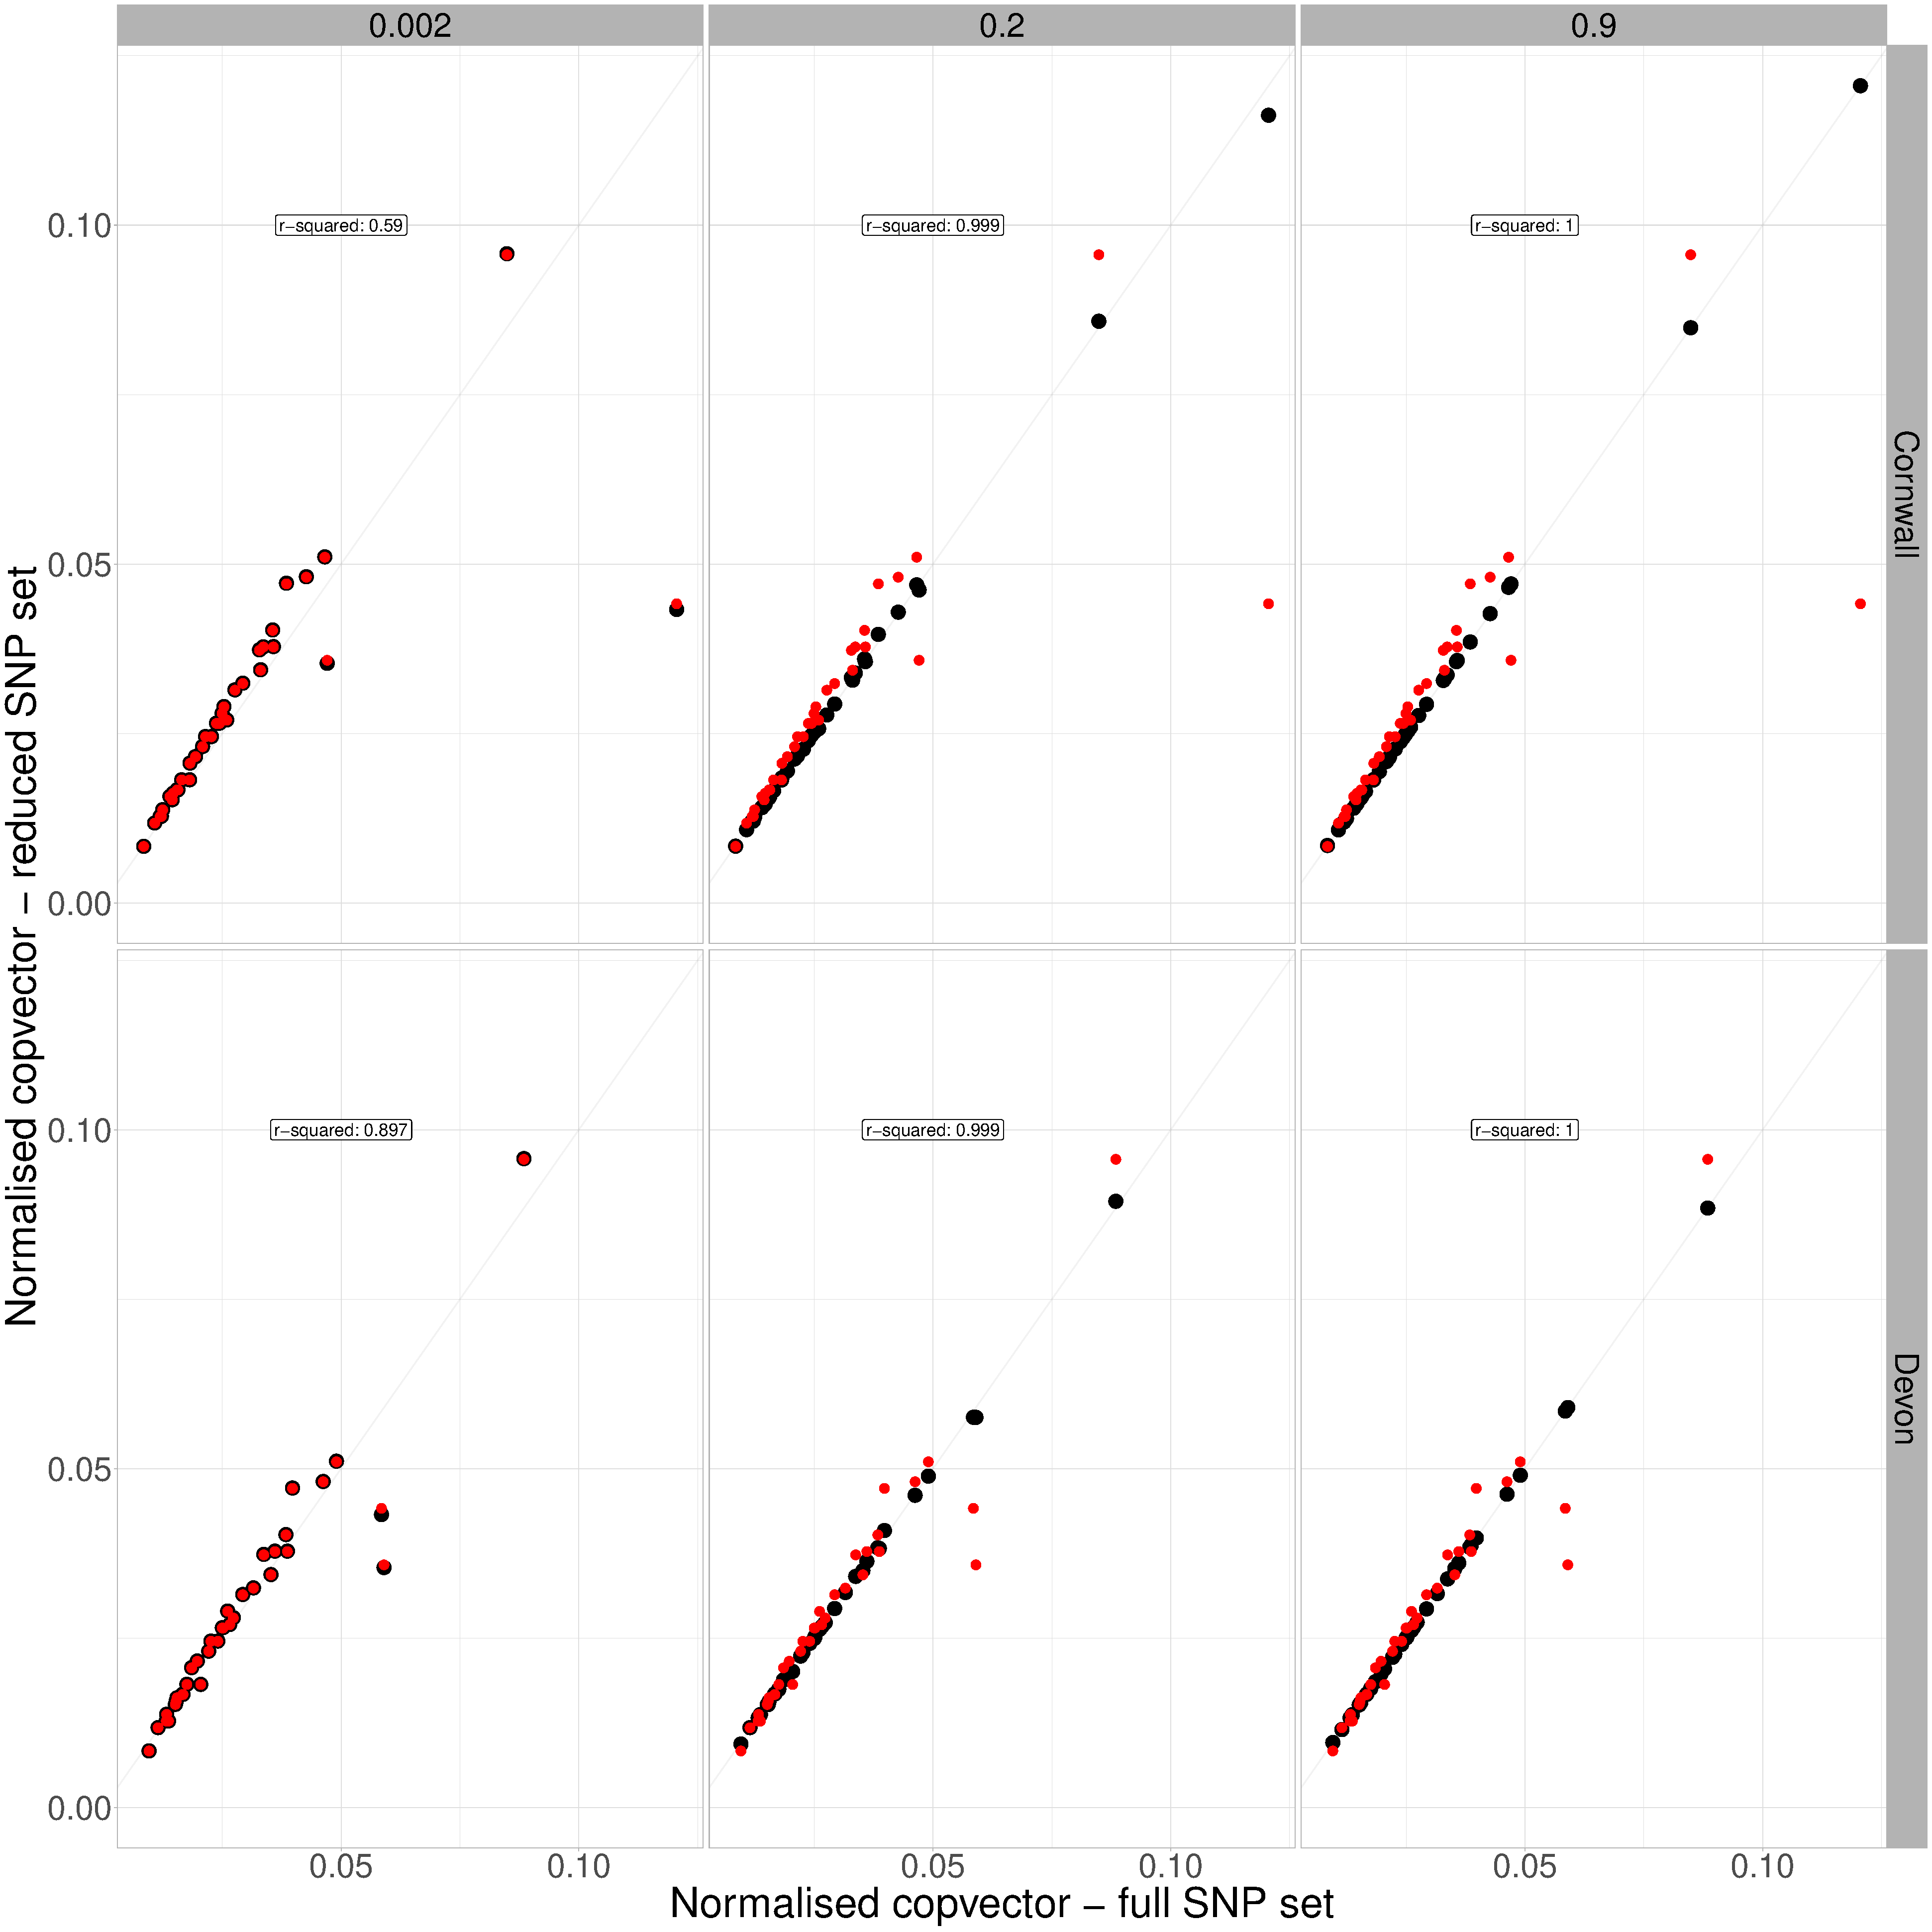
\includegraphics[width=1.0\textwidth]{../images/chapter1/Devon_Cornwall_copyvectors_sample_size_reduced.pdf}
    \caption{Relationship between copyvectors using reduced (y-axis) and full (x-axis) set of SNPs. Panels indicate different levels of reduced SNPs (0.002 = 0.002*full number of SNPS). Copyvectors were estimated by averaging across all individuals within each population (black points). Also shown in red are the sample sizes of each donor population.}
    \label{fig:Devon_Cornwall_copyvectors_sample_size_reduced}
\end{figure}

From visual inspection, 0.2 is the level of reducing SNPs in both Devon and Cornwall whereby the copyvector matches the same copyvector estimated from the full coverage of SNPs. Therefore, given populations of similar sizes in equivalent ancient individuals, we could expect to reduce the total number of SNPs 

Secondly, it is important to understand the effect of SNP density on the accuracy of copyvector estimation. To quantify this, I compared the copvectors estimated from different SNP densities, but roughly the same total number of SNPs. 

In this example, using the POBI dataset, at 0.02 density there are 9,548 SNPs in total across 6901.0cM, giving a mean density of 1.38 SNPs/cM. On the other hand, at 0.9 density, there are 6,777 SNPs across the 144.71cM long chromosome 22, giving a density of 46.83 SNPs/cM. Therefore, the SNPs on chromosome 22 are substantially more dense. Henceforth I will refer to the 0.02 density set of SNPs as the 'sparse' set and the 0.9 chromosome 22 set of SNPs as the 'dense' set. 

I performed 3 different paintings, all 3 using all the POBI counties as donors and individuals from Devon and Cornwall as recipients. The first painting used all chromosomes and all SNPs. The second painting used the 'sparse' SNP set. The third painting used the 'dense' SNP set. For all 3 paintings, the mean copyvector for Devon and Cornwall was estimated by taking the mean copyvector across all individuals within a population. 

\begin{figure}[htp]
    \centering
    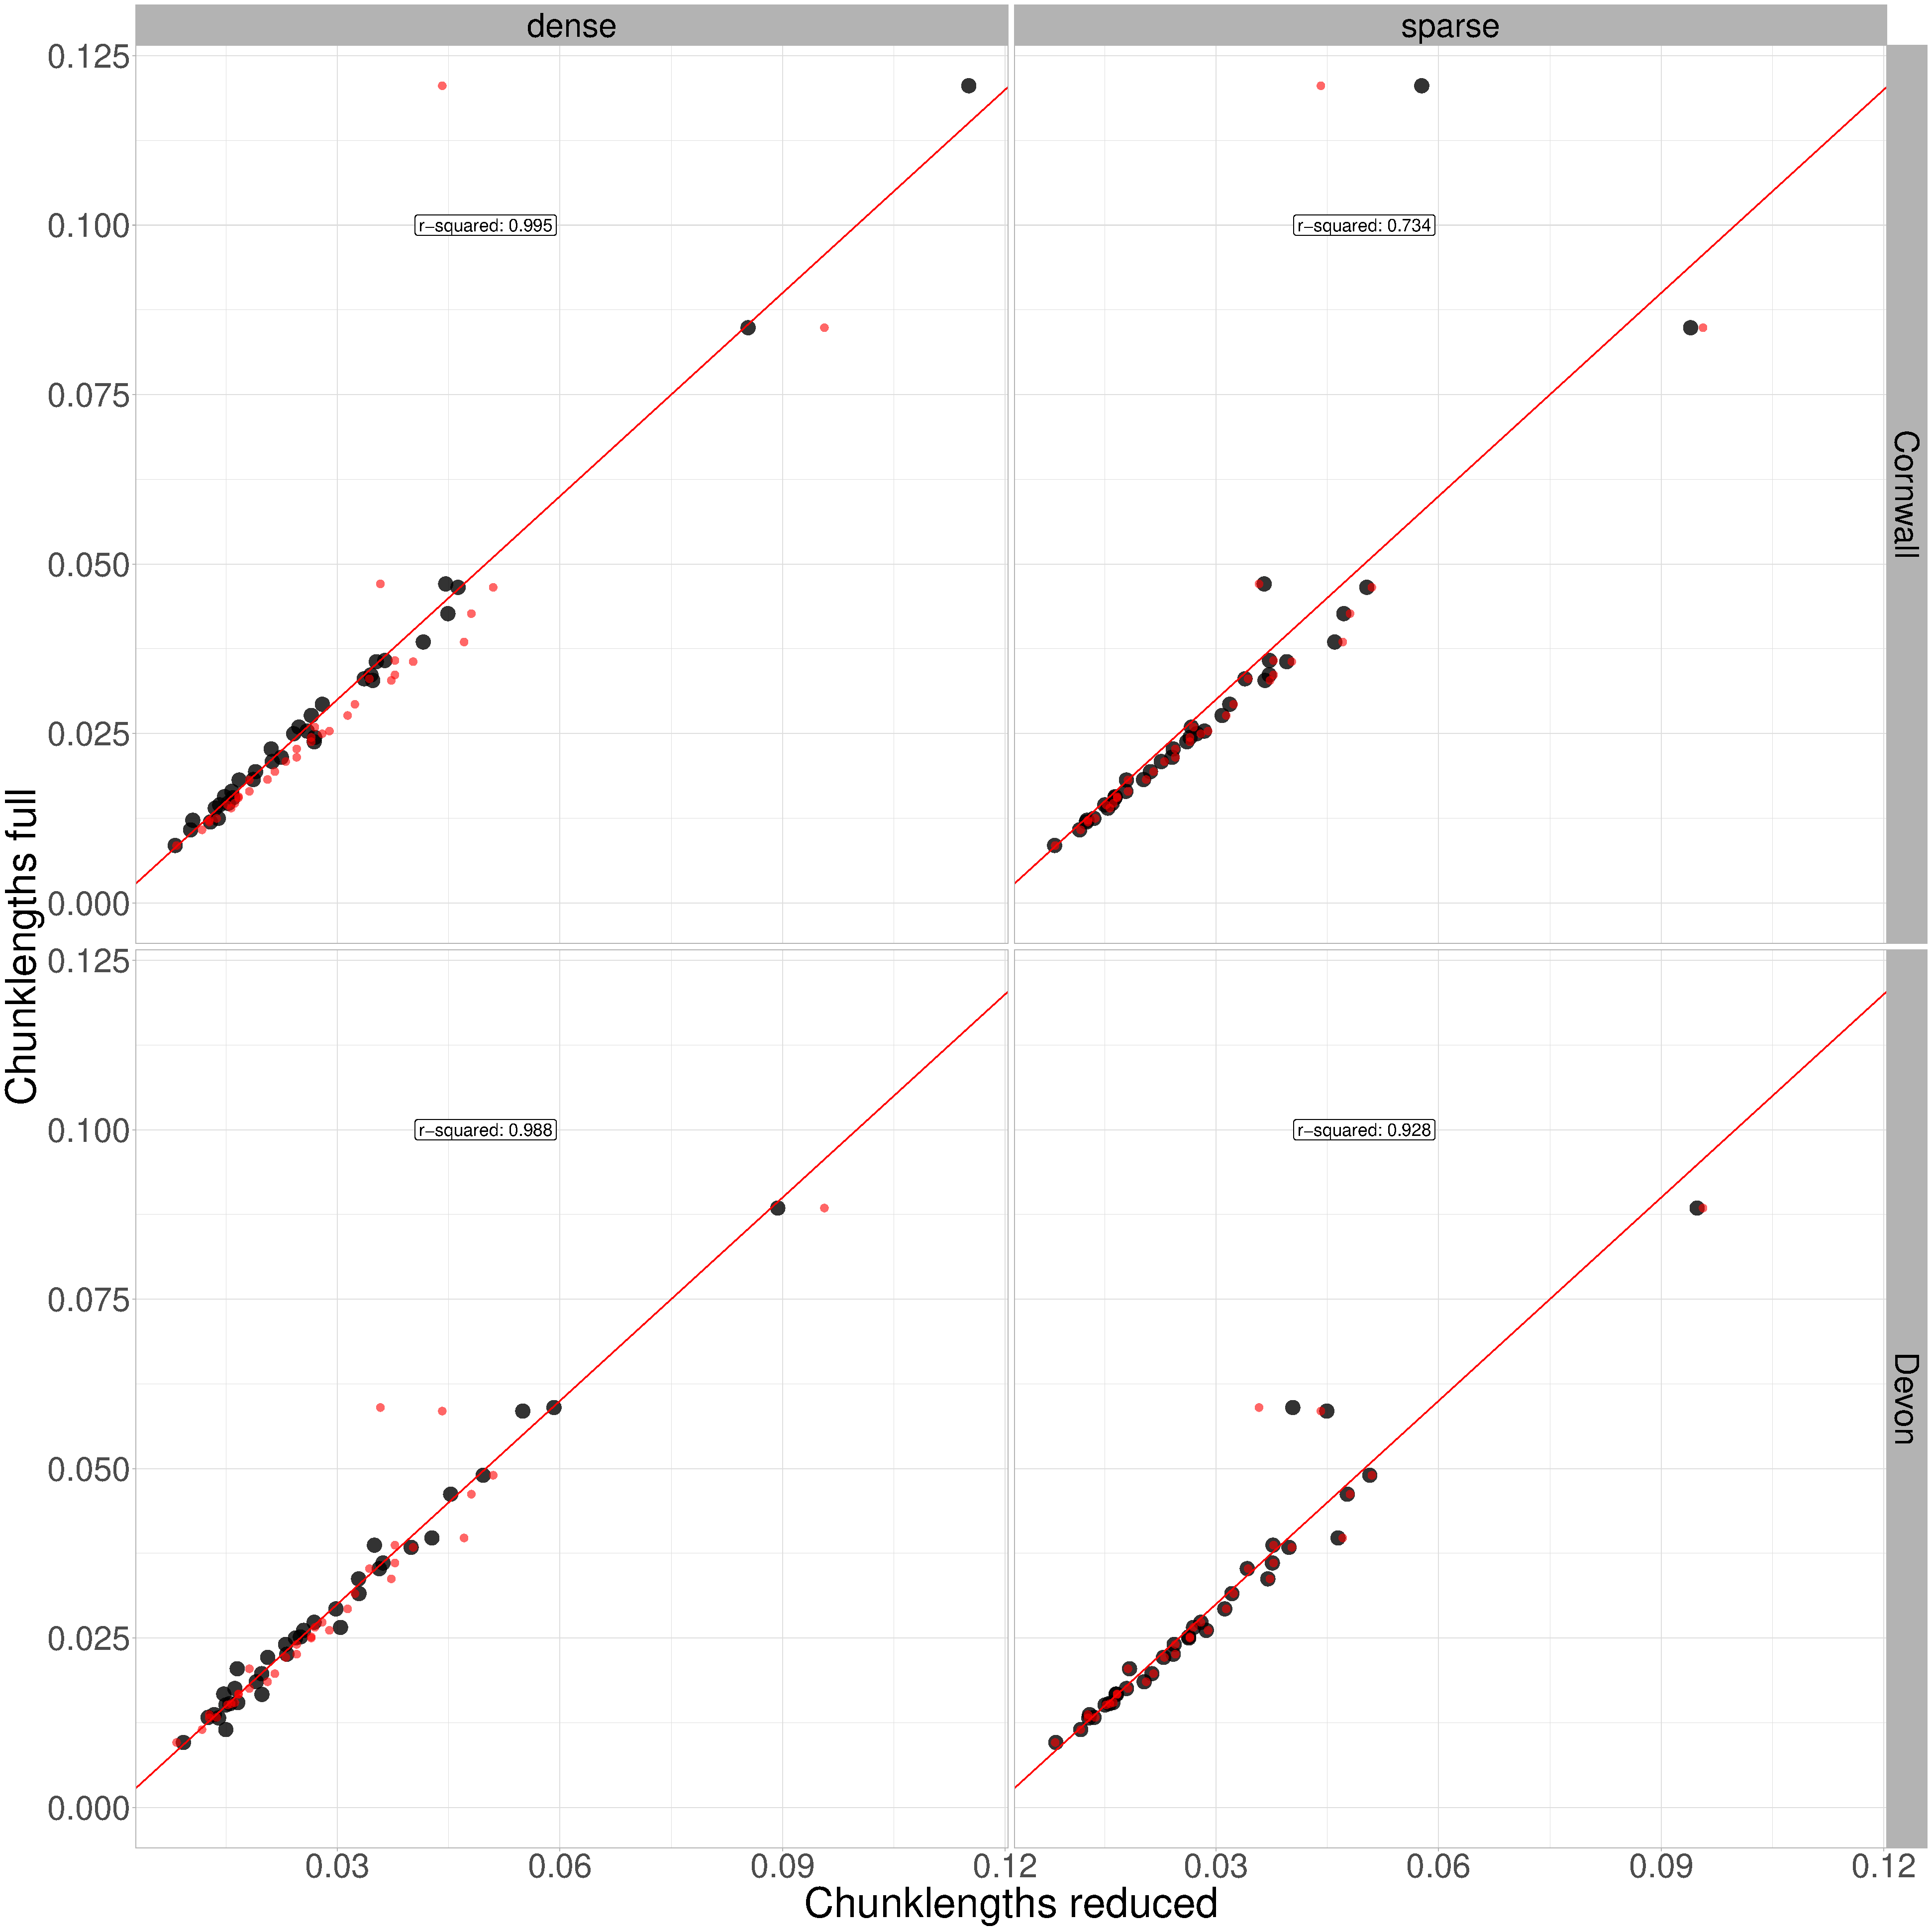
\includegraphics[width=1.0\textwidth]{../images/chapter1/dense_sparse_devon_cornwall_collapsed.pdf}
    \caption{Relationship between copyvectors using reduced (y-axis) and full (x-axis) set of SNPs. Panels indicate different levels of SNP density. Copyvectors were estimated by averaging across all individuals within each population (black points). Also shown in red are the sample sizes of each donor population.}
    \label{fig:dense_sparse_devon_cornwall_collapsed}
\end{figure}

Fig. \ref{fig:dense_sparse_devon_cornwall_collapsed} displays the relative copyvector accuracy between using a dense and sparse set of SNPs. The r-squared value is higher using the denser set of SNPs, suggesting using denser SNPs can more accurately estimate the copy vector than the same number of more sparse SNPs.This also suggests that, if chosen well, a fraction of the original number of SNPs can recover a large amount of the original information. 

In fact, it is possible to reduce the density on the 'dense' of SNPs down to 0.3 and still mitigate the effect of regression to the prior.

However, the relationship between the 'dense' copyvector and full coverage copyvector appears to be influenced by the number of individuals in the recipient population. Reducing the number of individuals within the recipient population (i.e. the number of individuals assigned to the population 'POBI:Cornwall' reduces the overall r-squared between the 'dense' and full coverage copyvectors Fig. \ref{fig:Ssparse_cornwall_collapsed_random_remove_inds}.

\begin{figure}[htp]
    \centering
    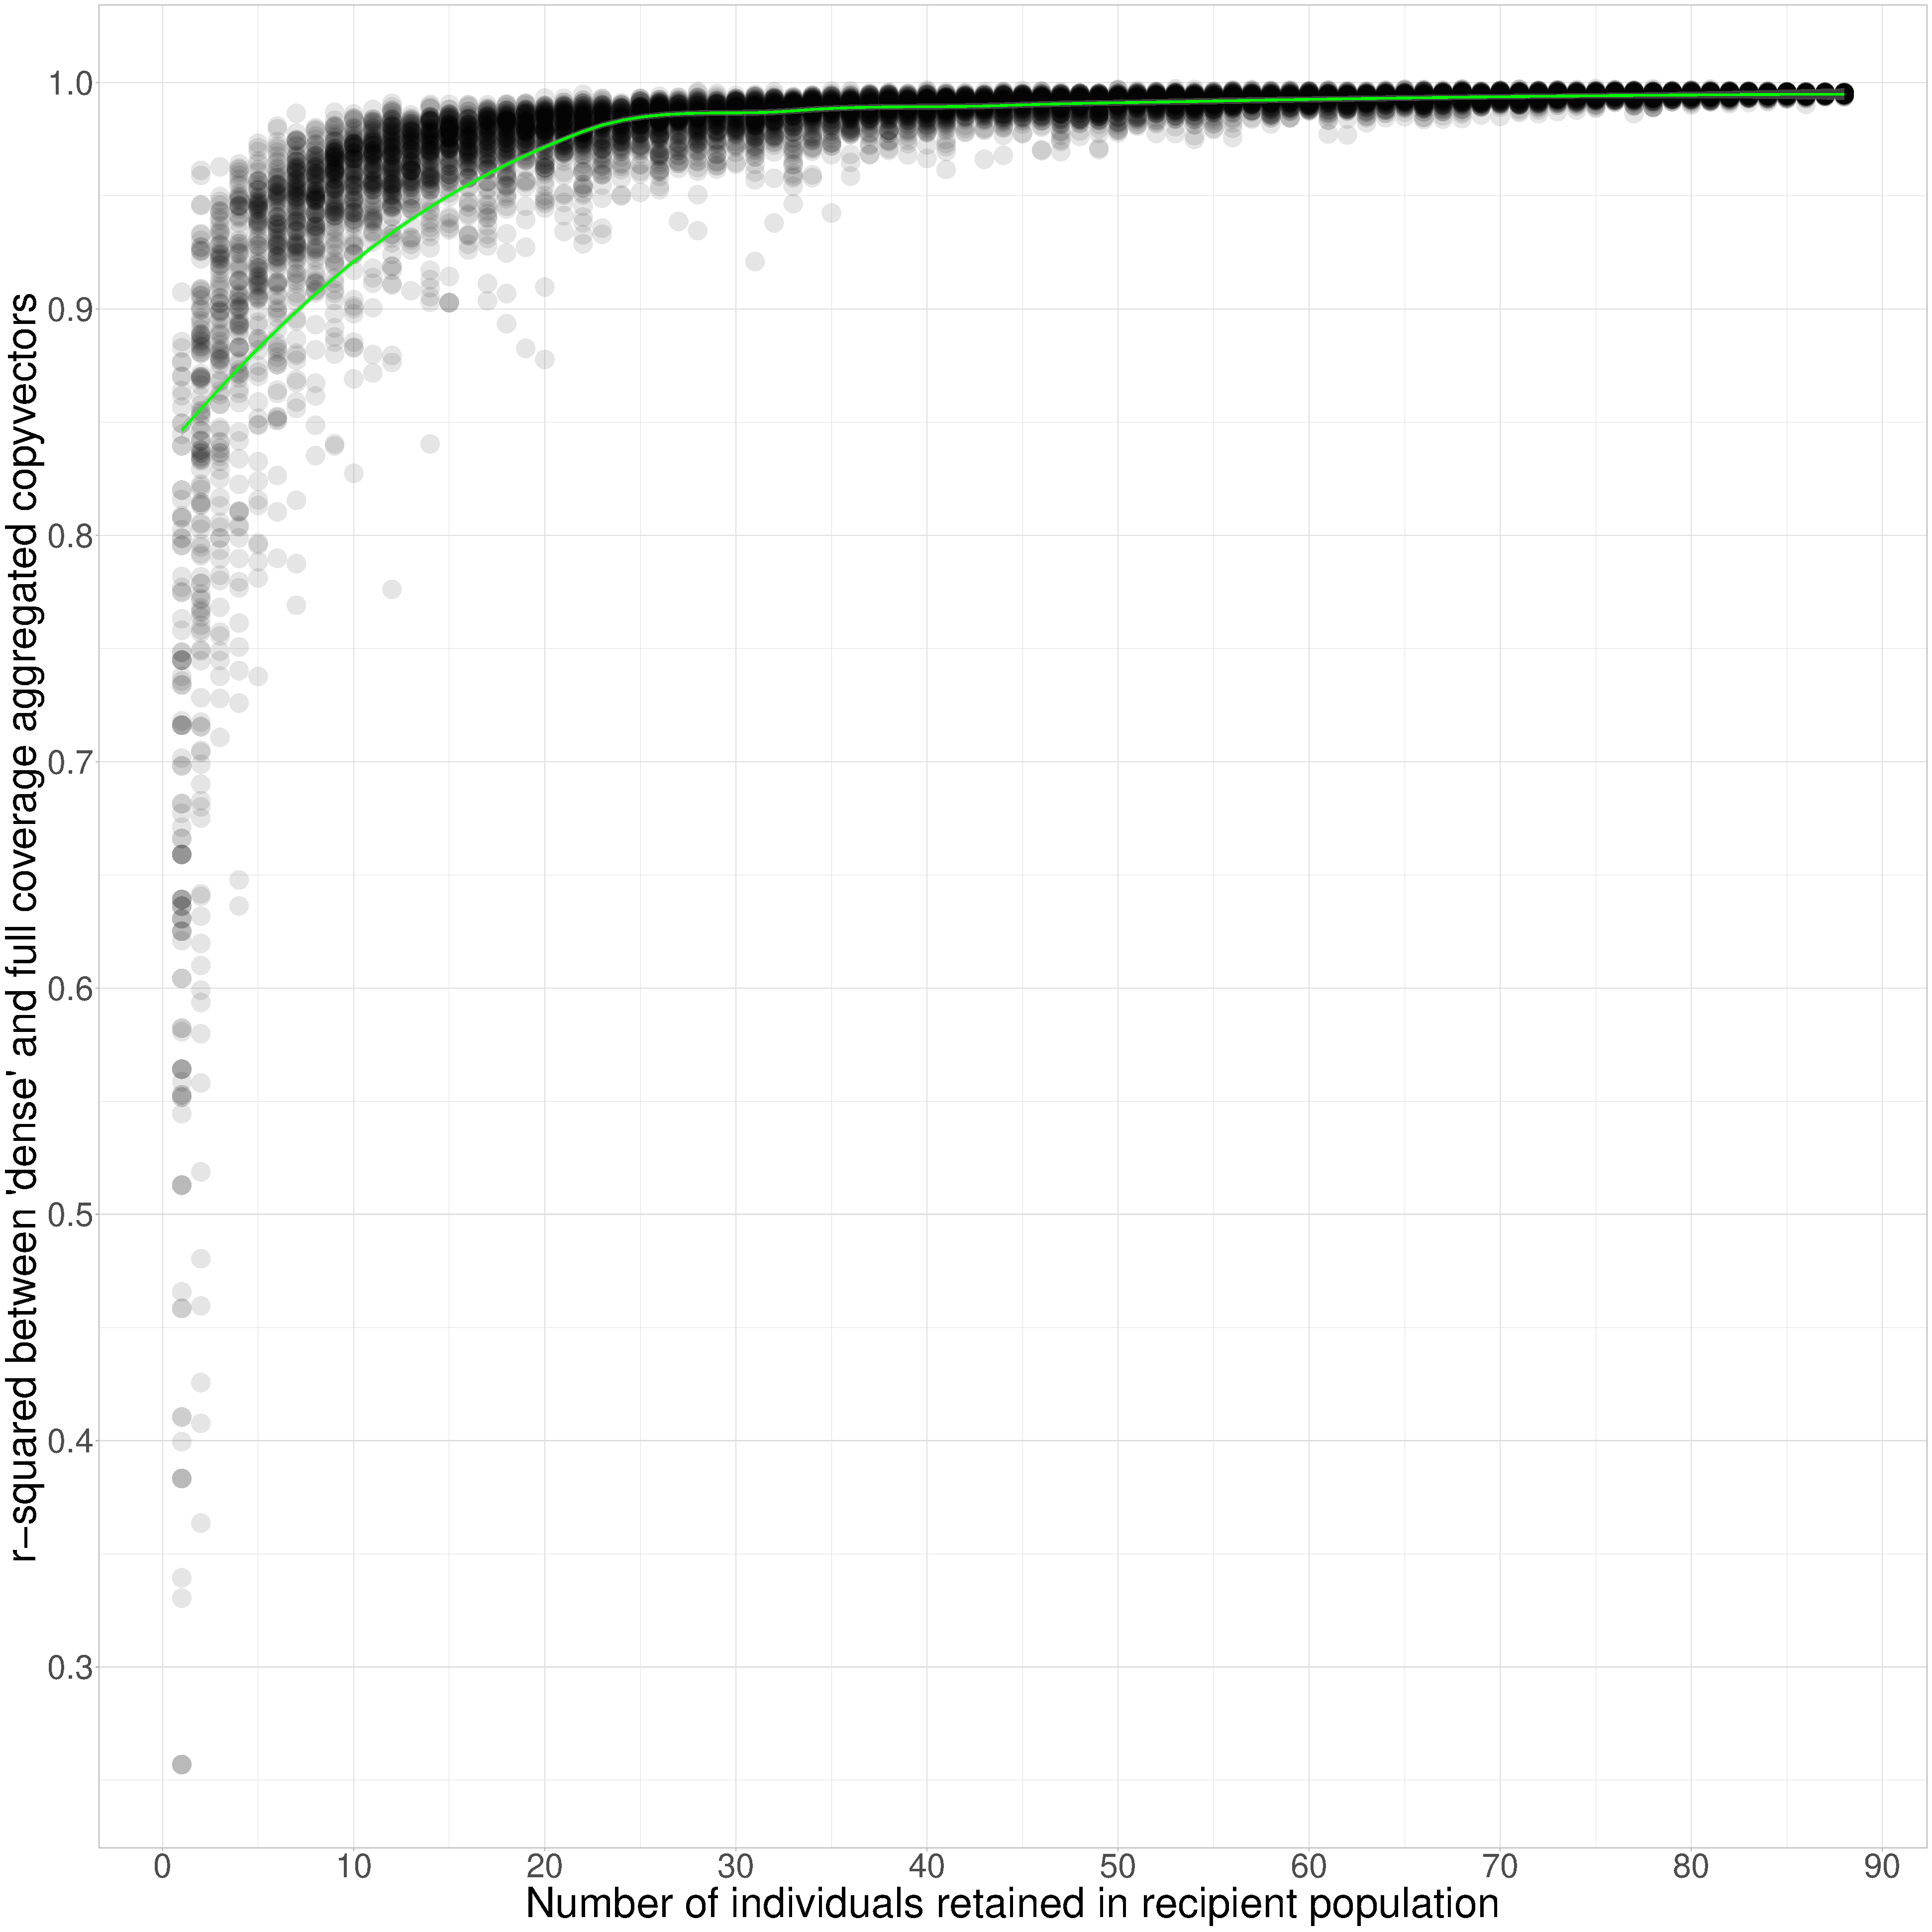
\includegraphics[width=1.0\textwidth]{../images/chapter1/Ssparse_cornwall_collapsed_random_remove_inds.pdf}
    \caption{R-squared between the copyvectors estimated from 'dense' and full SNP sets (y-axis) using different sample sizes (x-axis). 'Dense' SNP set corresponds to the SNPs located on chromosome 22 at 0.9 density. Copyvectors were estimated by aggregating $n$ randomly selected individuals within the population, corresponding to the x axis-value. Green line is local polynomial regression line. }
    \label{fig:Ssparse_cornwall_collapsed_random_remove_inds}
\end{figure}

\begin{figure}[htp]
    \centering
    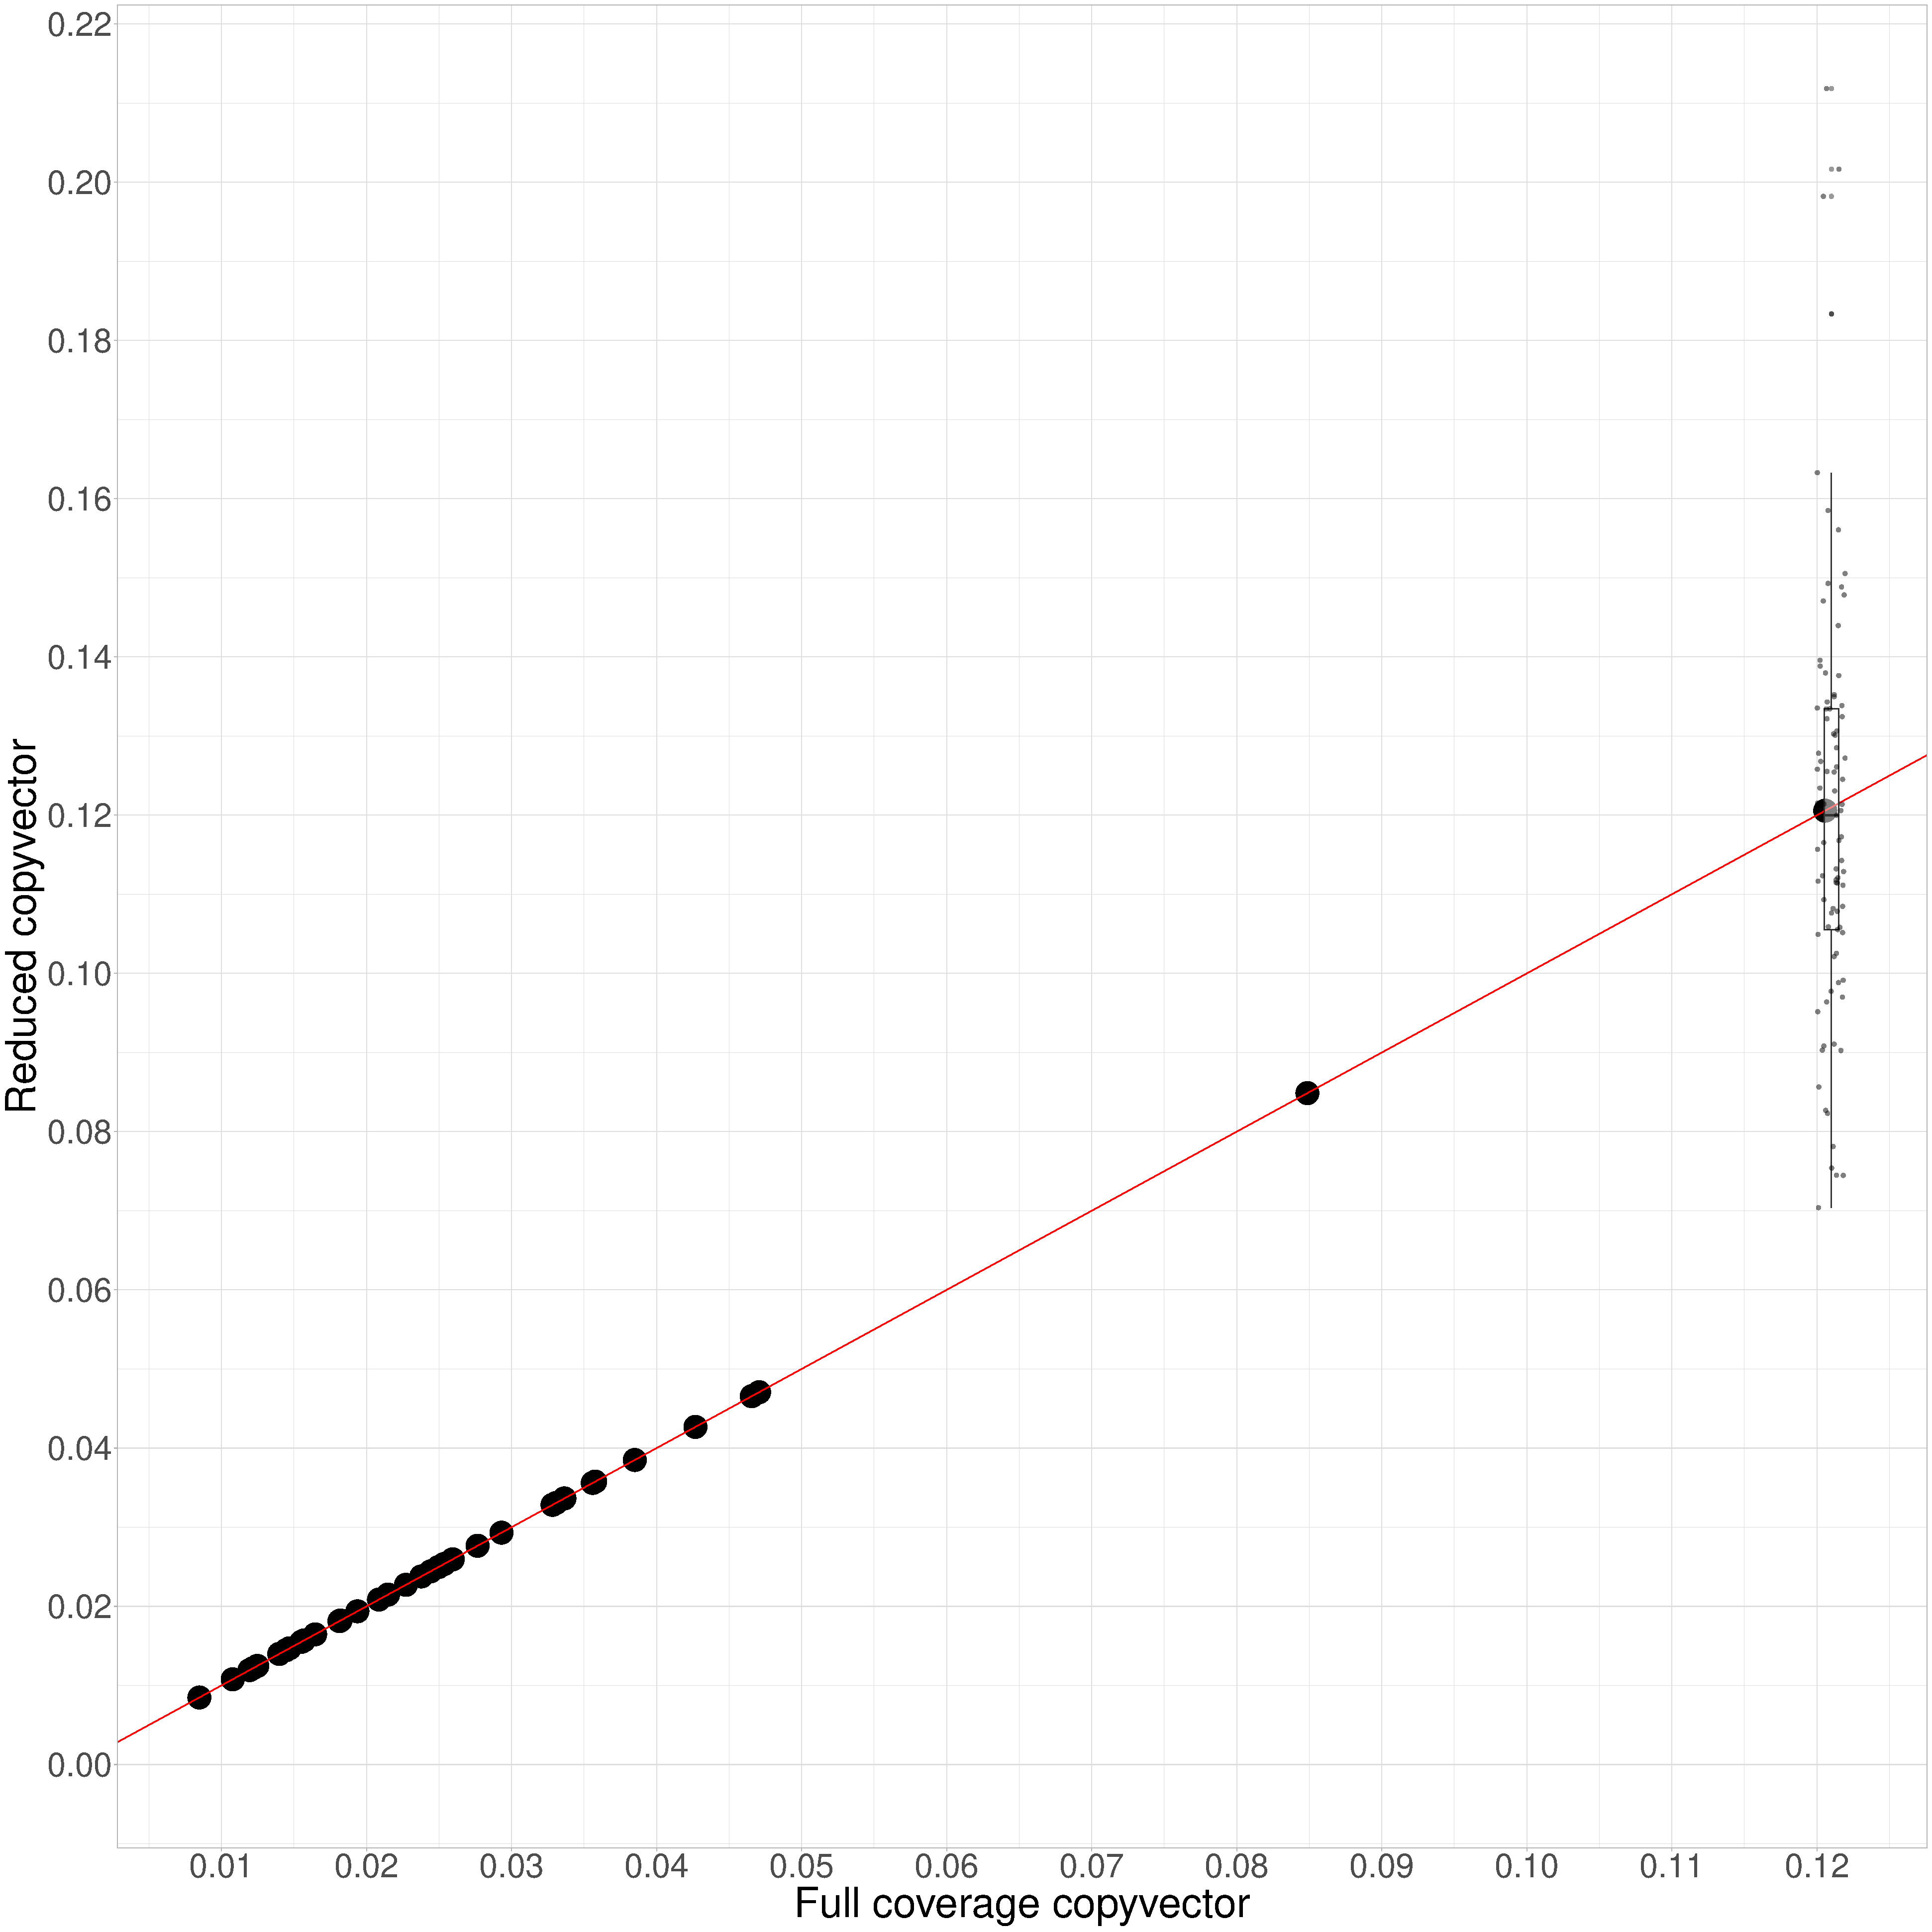
\includegraphics[width=1.0\textwidth]{../images/chapter1/dense_sparse_devon_cornwall_collapsed_scatterpoints.pdf}
    \caption{Aggregated copyvector for all individuals from Cornwall. Points correspond to the mean amount copied to different different POBI donor groups. Scattered points are the individual amounts each individual within the Cornwall group copies from the Cornwall donor group (i.e. self-copying).}
    \label{fig:dense_sparse_devon_cornwall_collapsed_scatterpoints}
\end{figure}

With this information in mind, we can consider its use for ancient DNA. The previous section showed that imputed SNPs are the primary cause of coverage-related bias. Therefore, if we can find dense regions of non-imputed genotypes at sufficient coverage, we may be able to recover a large amount of the haplotype information from low coverage (<0.5x) samples.

The previous section informed us that approximately 2259 SNPs spaced over on chromosome 22 was sufficient to recover haplotype information. To obtain the mean number of SNPs per chunk, we can calculate $\dfrac{\sum_{i=1}^{d} \sum_{j=1}^{r} (c_{ij})}{d*r} * n$, where $d$ is the number of donor individuals, $r$ is the number of recipient individuals, $n$ is the number of SNPs over the region of interest and $c_{ij}$ is the number of chunks donated from donor $i$ to recipient $j$. In the case of chromosome 22 at density 0.3, this yields 572 SNPs per chunk. We can also calculate the mean segment length as $L \div C$, (element-wise division) where $C$ is the chunkcounts matrix and $L$ is the  chunklengths matrix, which gives the average segment length each donor contributes towards each recipient. Taking the mean across all donors and recipients yields a value of 0.77cM. 

The genetic map used in the analysis was 70cM and there are 545,870 corresponding to a density of 1 SNP per 0.00012cM. 

NB: Didn't have time to finish this part. 


\subsection{Incorporating the sample size vector into SOURCEFIND}

NB: Not sure if to include this if it didn't work well?








